%!TEX root = ../PhD_thesis__Lilian_Besson

% \chapter{SMPyBandits: a state-of-the-art Python library to simulate MAB problems}
\chapter{SMPyBandits: our Python library to simulate MAB problems}
\label{chapter:3}

\graphicspath{{2-Chapters/3-Chapter/Images/}{2-Chapters/3-Chapter/logs/}{2-Chapters/3-Chapter/SMPyBandits_paper.git/plots/}}

\TODOL{Si j'ai le temps, je peux améliorer les expériences faites en 3.3 et 3.4. C'est déjà suffisant comme ça, je peux juste faire mieux !}

\abstractStartChapter{}%
%
SMPyBandits is a Python package I have developed since the beginning of my PhD.
It is designed to allow easy and fast numerical simulations on single-player and multi-players Multi-Armed Bandits (MAB) algorithms.
It is the most exhaustive open-source implementation of state-of-the-art algorithms and different kinds of MAB models.
%
This chapter details the organization of the library, what it implements in terms of arm distributions, models, algorithms and visualizations.
Then we use it to perform a numerical comparisons of the main state-of-the-art single-player MAB algorithms, and a study to compare time and memory costs of the main algorithms.

\minitocStartChapter{}

% ----------------------------------------------------------------------------
\section{Introduction}
\label{sec:3:Introduction}

% This chapter is intended as a long version of the paper presenting SMPyBandits that I wrote in Summer 2018, see https://hal.inria.fr/hal-01840022

% SMPyBandits is the most complete open-source implementation of state-of-the-art algorithms and models of Multi-Armed Bandits.
% It aims at being extensive, simple to use and maintain, with a clean and perfectly documented codebase. But most of all it allows fast prototyping of simulations and experiments, with an easy configuration system and command-line options to customize experiments while starting them (see below for an example).

Since December $2016$ I worked regularly on the SMPyBandits library, which is a Python package  designed to allow easy and fast numerical simulations on single-player and multi-players Multi-Armed Bandits (MAB) algorithms.
%
This library is by far the most exhaustive open-source implementation of state-of-the-art algorithms and different kinds of MAB models.
It aims at being exhaustive, simple to use and maintain, and has a clean and well documented codebase, and it uses the popular open-source Python language.
It allows fast prototyping of simulations, with an easy configuration system and command-line options to customize experiments.
Experiment results are saved in an optimized binary format (HDF5) as well as high quality plots of useful visualizations.
%
More than two years of active development have shown how easy it can be to add new algorithms, new arm distributions, and new bandit models (\eg, Markov or non-stationary).
It is hosted on GitHub, and uses the state-of-the-art development technologies, by using two online services of continuous integration to run automated tests and to build its online documentation.

SMPyBandits stands for \emph{S}ingle- and \emph{M}ulti-\emph{P}layer \emph{Bandits} in P\emph{y}thon.
The library does not aim at being blazing fast or optimized in terms of memory usage, as it comes with a Python implementation \cite{python}, and uses only standard open-source Python packages (\ie, no hard to install dependencies).
Some critical parts are also available as a \texttt{C} Python extension, and the just-in-time Numba compiler \cite{numba} is used whenever it is possible, so we can note that we optimized the time efficiency of what could be (easily) optimized.
However if simulation speed really matters, one should rather refer to less exhaustive but faster implementations, like for example \cite{TorLibbandit} in \texttt{C++} or \cite{VishMABjl} in Julia. Note that both are not maintained anymore, and contain just a few algorithms for the simple stationary MAB model.

In this Chapter~\ref{chapter:3}, we start by presenting in Section~\ref{sec:3:presentationLibrary} the organization of the library.
We use the library to compare the most famous and most efficient single-player MAB algorithms in Section~\ref{sec:3:reviewSPAlgorithms},
then we discuss in Section~\ref{sec:3:timeAndMemoryCosts} about the time and memory costs the same algorithms.
The take away messages are two-fold:
from a practical point-of-view, it is usually advised to use the simplest algorithm and we advise to use \UCB{} (as we do in the next Chapter~\ref{chapter:4}),
and that for theoretical works where optimality of the MAB algorithm is analyzed, we advise to use \klUCB{} (as we do in the next Chapters~\ref{chapter:5} and \ref{chapter:6}).
% To also illustrate how one can easily extend the SMPyBandits library to add not only add new distributions or new algorithms.
% but also new bandit models, we detail in Section~\ref{sec:3:markovModels} how we added the possibility to simulate Markovian models (as introduced by \cite{Anantharam87b}).
%
Finally, in Appendix~\ref{sec:3:appendix} we include some small files showing how to use the library, and we conclude with some details regarding the use of parallel computing to speed-up simulations.


\paragraph{References.}
%
The code for SMPyBandits is hosted at \texttt{\href{https://GitHub.com/SMPyBandits/SMPyBandits/}{GitHub.com/SMPyBandits/SMPyBandits}}, its documentation is at \texttt{\href{https://SMPyBandits.GitHub.io/}{SMPyBandits.GitHub.io}}, and all the library is freely publicly released under the MIT open-source License.
This chapter is based on our article \cite{SMPyBanditsJMLR}.


% ----------------------------------------------------------------------------
\section{Presentation of the library}
\label{sec:3:presentationLibrary}

% I want to show what is SMPyBandits, what problems does it solve, what did I implement, how to use it.

We start by explaining how SMPyBandits simulates MAB problems, by detailing its components:
MAB problems (single- or multi-players),
and reward distributions.
%
We then detail how it implements MAB algorithms (\eg, \UCB),
and what kind of information is displayed, saved and plotted after a batch of simulations of bandit problems.
%
%
The main goal of the library is to be easily able to simulate MAB algorithms (\eg, three algorithms like \UCB, \klUCB{} and Thompson sampling) on one or more bandit models (single- or multi-players) defined by the number of arms $K$ and their distributions $(\nu_k)_{k\in[K]}$, for some time steps that range from $t=1$ to the horizon $T$.
After the simulation, the library then displays statistical summary of the (mean) rewards accumulated by each algorithm, as well as regret and other visualizations.
The same problem is simulated for $N$ independent repetitions (\eg, $N=100$) in order to show mean results with low variances.


\subsection{Single- and multi-players MAB problems}

For the classical single-player stochastic MAB model, as defined in Chapter~\ref{chapter:2},
a stochastic MAB problem is defined by $K \geq 2$ distributions $(\nu_k)_{k\in[K]}$ (also called arms),
used to generate the \iid{} samples $Y_{k,t} \sim \nu_k, \forall t$.
%
An agent chooses arm $A(t)\in[K]$ at time $t$ and observes the reward $r(t) = Y_{A(t),t}$ without knowing the other (hidden) rewards (in opposition to the full-information setting where $(Y_{1,t},\dots,Y_{K,t})$ is observed).
%
Her goal is to maximize $\sum_{t=1}^T r(t)$, which require to trade off between exploring the unknown $K$ arms, exploiting the arm which is currently estimated to be the best one.

\paragraph{Simulation loop for single-player MAB.}
%
Any simulation library targeting single-player bandit problems must implement at least three components:
reward distributions, MAB algorithms, and a simulation loop that essentially looks like this.
% \begin{itemize}
    % \item
    First, initialize the MAB problem and one or more algorithms,
    % \item
    Then, for $t=1$ to $t=T$ (known before hand), repeat the following block (for each algorithm). Ask algorithm $\cA$ her chosen arm $A(t)$, then sample a (random) reward $r(t)$ (\iid) from distribution $\nu_{A(t)}$, and finally feeds the observation $(A(t), r(t))$ to the algorithm.
    % \item
    At the end, compute the cumulated reward, the regret, then plot visualizations etc.
% \end{itemize}
%
Note that the second step should be repeated a large number of times (\eg, $N=100$), in order to study \emph{mean} regret and not only the regret in one single trajectory.
If one wants to compare algorithms on a same problem, it is possible to sample all the rewards $(Y_{k,t})_{k\in[K], t\in[T]}$ before-hand, and store them so that for each repetition of the simulation, the randomness from the environment (\ie, the rewards) has the same impact on all the algorithms (with the option \texttt{configuration["cache\_reward"] = True}).


\paragraph{Simulation loop for multi-players MAB.}
%
For Cognitive Radio dealing with OSA problems and other applications, an extension is to consider $M\geq2$ players, interacting on the same $K$ arms.
Whenever two or more players select the same arm at the same time (\eg, for OSA, the same frequency channel), they all suffer from a radio collision.
%
Different collision models have been proposed, and the simplest one consists in giving a $0$ reward to each colliding players.
Without any centralized supervision or coordination between players, they must learn to access the $M$ best resources (\ie, arms with highest means) without collisions.
We refer to Chapter~\ref{chapter:5} which introduces the multi-players bandit model.

SMPyBandits implements all the collision models found in the literature (in the module \texttt{\href{https://SMPyBandits.GitHub.io/docs/Environment.CollisionModels.html}{Environment.CollisionModels}}), as well as all the algorithms known by the authors (in the module \texttt{\href{https://SMPyBandits.GitHub.io/docs/PoliciesMultiPlayers.html}{PoliciesMultiPlayers}}).
%
In particular, it includes
\texttt{rhoRand}
% (\texttt{\href{https://SMPyBandits.GitHub.io/docs/PoliciesMultiPlayers.rhoRand.html}{PoliciesMultiPlayers.rhoRand}})
from \cite{Anandkumar11},
\texttt{MEGA}
% (\texttt{\href{https://SMPyBandits.GitHub.io/docs/Policies.MEGA.html}{Policies.MEGA}})
from \cite{Avner15},
\texttt{MusicalChair}
% (\texttt{\href{https://SMPyBandits.GitHub.io/docs/Policies.MusicalChair.html}{Policies.MusicalChair}})
from \cite{Rosenski16},
and our state-of-the-art algorithms
\texttt{RandTopM}
% (\texttt{\href{https://SMPyBandits.GitHub.io/docs/PoliciesMultiPlayers.RandTopM.html}{PoliciesMultiPlayers.RandTopM}})
and \texttt{MCTopM}
% (\texttt{\href{https://SMPyBandits.GitHub.io/docs/PoliciesMultiPlayers.MCTopM.html}{PoliciesMultiPlayers.MCTopM}})
from \cite{Besson2018ALT}, and more recent solutions.
For comparison, realistic (\eg, \UCB{} for multiple play) or full-knowledge \emph{centralized} algorithms are also implemented.

Any simulation library targeting multi-players bandit problems must implement at least another component:
% a collision model, and
a simulation loop that essentially looks like this.
% \begin{itemize}
    % \item
    First, initialize the MAB problem with $M$ players, and one or more cohorts of $M$ players (one player is one algorithm, usually $M$ times the same one),
    % \item
    For $t=1$ to $t=T$ (known before hand), repeat the following block (for each cohort). Ask each player $\cA^j$ her chosen arm $A^j(t)$, then query the collision model to know which player will get a zero reward (for a collision) and which player will get a random reward from the environment.
    Then, sample (random) feedback $Y_{k,t}$ (\iid) from distributions $\nu_{k}$, and compute the rewards $r^j(t)$ from the random feedback using the collision model.
    Finally, feed the observation $(A^j(t), Y_{A^j(t),t}, r^j(t))$ to player $j$, for all the $M$ players,
    %
    The default collision model is the most widely studied in the literature, where a player encounters a collision (\ie, received a zero reward $r^j(t)=0$) if she is not the only one to have chosen an arm $k=A^j(t)$, otherwise $r^j(t)=Y_{A^j(t),t}$ if she is the only one playing this arm.
    % \item
    At the end, compute the accumulated reward, the regret, then plot visualizations etc.
% \end{itemize}


\subsection{Reward distributions}
%
We focus on one dimensional distributions (\ie, $r(t)\in\R$), implemented in the \texttt{\href{https://smpybandits.github.io/docs/Arms.html}{Arms}} module.
The library supports discrete distributions: \emph{Bernoulli} (\texttt{\href{https://smpybandits.github.io/docs/Arms.Bernoulli.html}{Bernoulli}}), \emph{binomial} (\texttt{\href{https://smpybandits.github.io/docs/Arms.Binomial.html}{Binomial}}), \emph{Poisson} (\texttt{\href{https://smpybandits.github.io/docs/Arms.Poisson.html}{Poisson}}), and a generic \emph{discrete} distribution (\texttt{\href{https://smpybandits.github.io/docs/Arms.DiscreteArm.html}{DiscreteArm}}),
as well as continuous distributions,
which can be truncated to an interval $[a,b]$ or have unbounded support ($\mathbb{R}$):
\emph{exponential} (\texttt{\href{https://smpybandits.github.io/docs/Arms.Exponential.html}{Exponential}}), \emph{gamma} (\texttt{\href{https://smpybandits.github.io/docs/Arms.Gamma.html}{Gamma}}), \emph{Gaussian} (\texttt{\href{https://smpybandits.github.io/docs/Arms.Gaussian.html}{Gaussian}}) and \emph{uniform} (\texttt{\href{https://smpybandits.github.io/docs/Arms.Uniform.html}{Uniform}}).
%
The default is to use the same distribution for the $K$ arms, as this is the setting studied in the literature,
but it also possible to mix them.
%  (\eg, one arm is Bernoulli-distributed and another).
%  (see for instance Figure~\ref{fig:25:HarderMixed}).
%
For instance the following code in Code~\ref{lst:3:pythonCodeCreateProblem} creates three arms, following Bernoulli distributions, with respective means $0.1, 0.5, 0.9$, and a \texttt{MAB} object which encapsulates the problem.
We give another example for \emph{truncated} Gaussian distributions on $[0,1]$, and a visualization of a histogram of $10000$ rewards, below in Figure~\ref{fig:3:exampleOfRewards}.

% https://tex.stackexchange.com/a/12430/
\begin{small}
\begin{listing}[h!]
    \begin{minted}[linenos=true,numbersep=5pt,frame=lines,framesep=2mm]{python}
from SMPyBandits.Arms import *
arm1 = Bernoulli(0.1)
arm2 = Bernoulli(0.5)
arm3 = Bernoulli(0.9)

means = [0.1, 0.5, 0.9]
from SMPyBandits.Environment import MAB
bernoulli_problem = MAB([arm1, arm2, arm3])
# but also
bernoulli_problem = MAB({'arm_type': Bernoulli, 'params': means})

gaussian_problem = MAB({'arm_type': Gaussian, 'params': means})
gaussian_problem.plotHistogram()  # display the histogram shown below
    \end{minted}
    \caption{Example of Python code to create Bernoulli and Gaussian arms, a MAB problem with $K=3$ arms, a plot a histogram of rewards, with SMPyBandits.}
    % \captionof{listing}{Example of Python code to create Bernoulli and Gaussian arms, a MAB problem with $K=3$ arms, a plot a histogram of rewards, with SMPyBandits. \label{lst:3:pythonCodeCreateProblem}}
    \label{lst:3:pythonCodeCreateProblem}
\end{listing}
\end{small}

\begin{figure}[h!]  % [htbp]
	\centering
	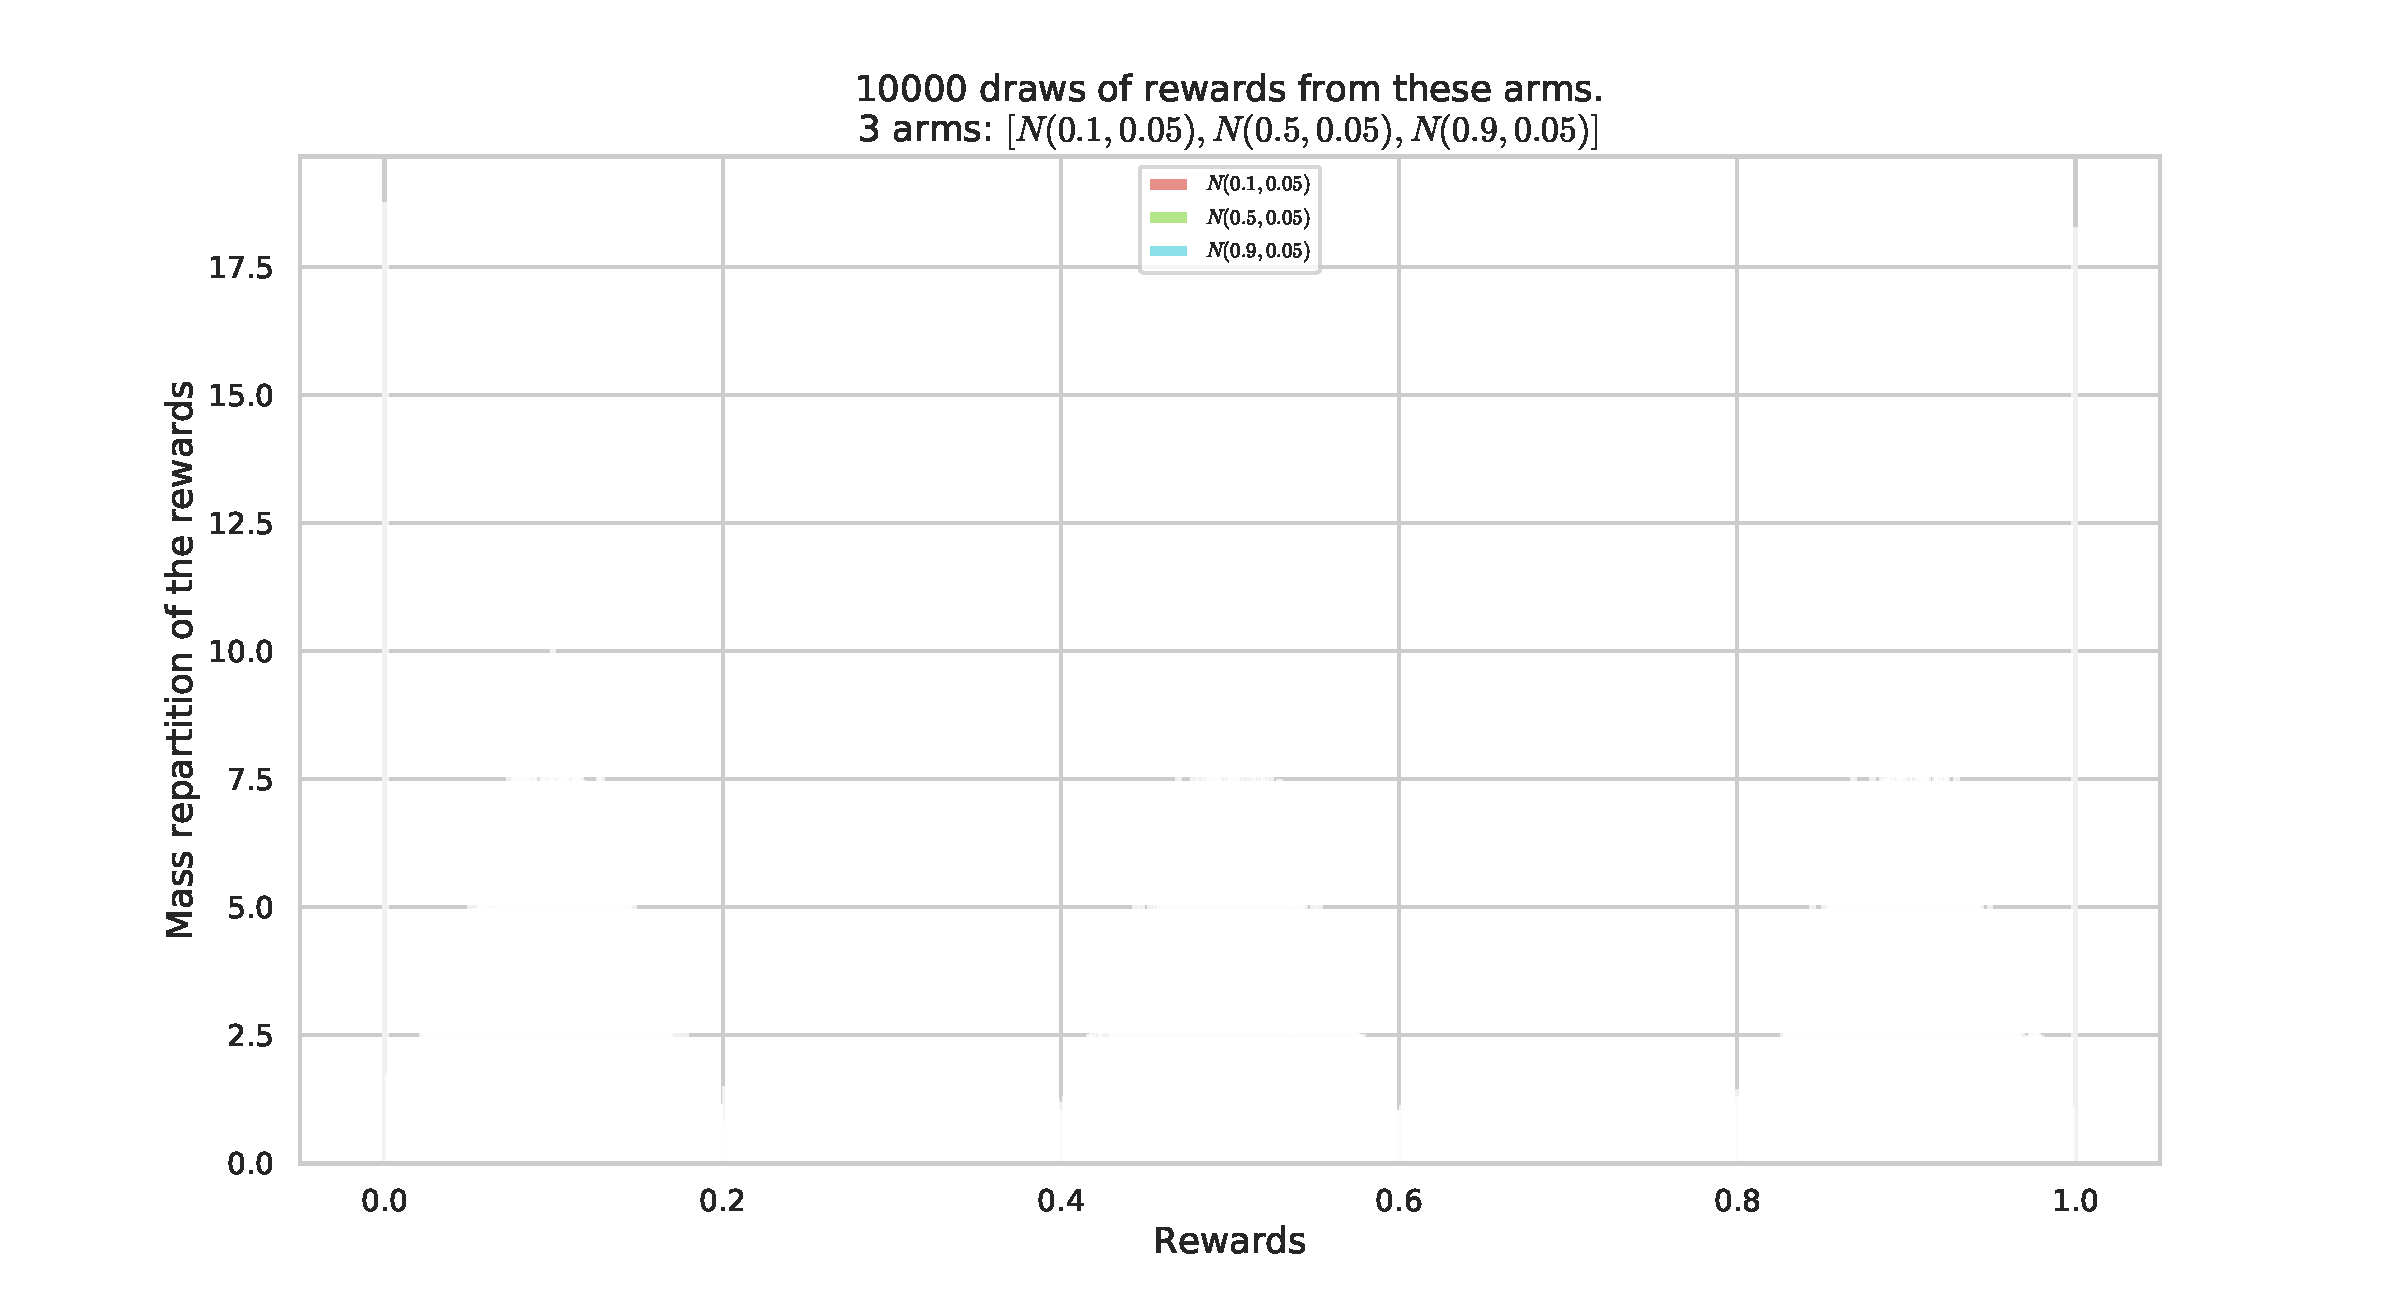
\includegraphics[width=0.75\linewidth]{exampleOfRewards.pdf}
	\caption{Histogram of $10000$ \iid{} rewards obtained from three arms with a Gaussian distribution truncated to $[0,1]$, of respective means $0.1$ (in \textcolor{red}{red}), $0.5$ (in \textcolor{green}{green}) and $0.9$ (in \textcolor{blue}{blue}).}
	\label{fig:3:exampleOfRewards}
\end{figure}

For more details, an interested reader can refer to the following Jupyter notebook \cite{jupyter}:
\href{https://smpybandits.github.io/notebooks/Easily_creating_MAB_problems.html}{\texttt{SMPyBandits.GitHub.io/notebooks/Easily\_creating\_MAB\_problems.html}}.

We have not yet added support for higher dimensional distributions of rewards, such as linear bandits, but it would be an interesting extension of SMPyBandits.
%
However, note that our library does support finite-state real-valued Markov MAB models, where arms correspond to Markov chains \cite{Norris98}, in the two \emph{rested}/\emph{restless} variants, as introduced by \cite{Anantharam87b}.


\subsection{Multi-Armed Bandits algorithms}

SMPyBandits is a complete open-source implementation of single-player (classical) bandit algorithms,
containing over 65 algorithms (in the module \texttt{\href{https://SMPyBandits.GitHub.io/docs/Policies.html}{Policies}}).
It uses a well-designed hierarchical structure and class inheritance scheme (as detailed on the various UML diagrams shown on the \texttt{\href{https://SMPyBandits.GitHub.io/uml_diagrams/README.html}{uml\_diagrams}} folder) to minimize redundancy in the codebase.
For instance, most existing algorithms are index policies (see Algorithm~\ref{algo:2:indexPolicy}), and new ones are easily written by inheriting from the \texttt{IndexPolicy} class (\texttt{\href{https://SMPyBandits.GitHub.io/docs/Policies.IndexPolicy.html}{Policies.IndexPolicy}}).
% They compute an index $U_k(t)\in\mathbb{R}$ for each arm $k$ at time $t$, and play $A(t) \in \arg\max_k U_k(t)$.
For instance the code specific to $\UCB_1$ (with $\alpha=2$) is as written and fully documented in a file as short as this:

% https://tex.stackexchange.com/a/12430/
\begin{small}
% \begin{listing}[h!]
    \inputminted[linenos=true,numbersep=5pt,frame=lines,framesep=2mm]{python3}{2-Chapters/3-Chapter/src/example_of_a_IndexPolicy_UCB.py}
    % \caption{Small snippet of code defining the UCB algorithm, as a simple example of an Index Policy.}
    \captionof{listing}{Code defining the $\UCB_1$ algorithm, as a simple example of an Index Policy\label{lst:3:smallIndexPolicy}.}
    % \label{lst:3:smallIndexPolicy}
% \end{listing}
\end{small}


\subsection{Summary of the features}

With this numerical framework, simulations can run on a single CPU or a multi-core machine using joblib \cite{joblib},
% (see Appendix~\ref{sub:3:parallelSimulations}),
and summary plots are automatically saved as high-quality PNG, PDF and EPS, using matplotlib \cite{matplotlib} and seaborn \cite{seaborn}.
Raw data from each simulation is also saved in an HDF5 file, using h5py \cite{h5py}, an efficient and compressed binary format, to allow easy post-mortem manipulation of any simulation results.
Making new simulations is very easy, one only needs to write a configuration script (\texttt{configuration.py}), without needing a complete knowledge of the internal code architecture.


\subsection{Documentation of the library}

A complete documentation, for each algorithm and the entire codebase, is available online at
% even including the constants in the different configuration files:
\texttt{\href{https://SMPyBandits.GitHub.io}{SMPyBandits.GitHub.io}}.
It uses the Sphinx software \cite{sphinx}, and the content is directly written in the Python files as docstrings (in \texttt{"""\dots"""}, see in the example of Code~\ref{lst:3:smallIndexPolicy} given above), so users have access to the documentation from within their IDE or the Python console.
The most interesting component of the library is the many MAB algorithms being implemented: for each of them, the documentation gives a reference to a research paper (\eg, \cite{Auer02} for \texttt{UCB} in Code~\ref{lst:3:smallIndexPolicy}), as well as a bird-eye view of its behavior.
For most algorithms, especially for index policies, the internal variables of the implementation are carefully linked to the notations of each paper, and formulas explaining the way the algorithm selects its arm are usually given.
Whenever it is needed, we also included warnings or information about the empirical performance of the more costly algorithms.

The documentation also contains extensive examples of all intermediate numerical functions, that are also used as tests (using \texttt{doctest.testmod} from the standard library).
For example, Figures~\ref{fig:3:twoScreenshotsOfTheDocumentation} and \ref{fig:3:twoMoreScreenshotsOfTheDocumentation} below show four screenshots from the documentation.
We show the main page, the list of algorithms in the \texttt{Policies} module, an example of the documentation of one algorithm (for the \klUCB-Switch algorithm from \cite{GarivierHadiji2018}), and a page detailing the API and organization of the library as well as instructions to follow if someone wants to implement a new model or a new algorithm.


% FIXME?
\vfill{}
% FIXME?

\begin{figure}[h!]  % [htbp]
    \centering
	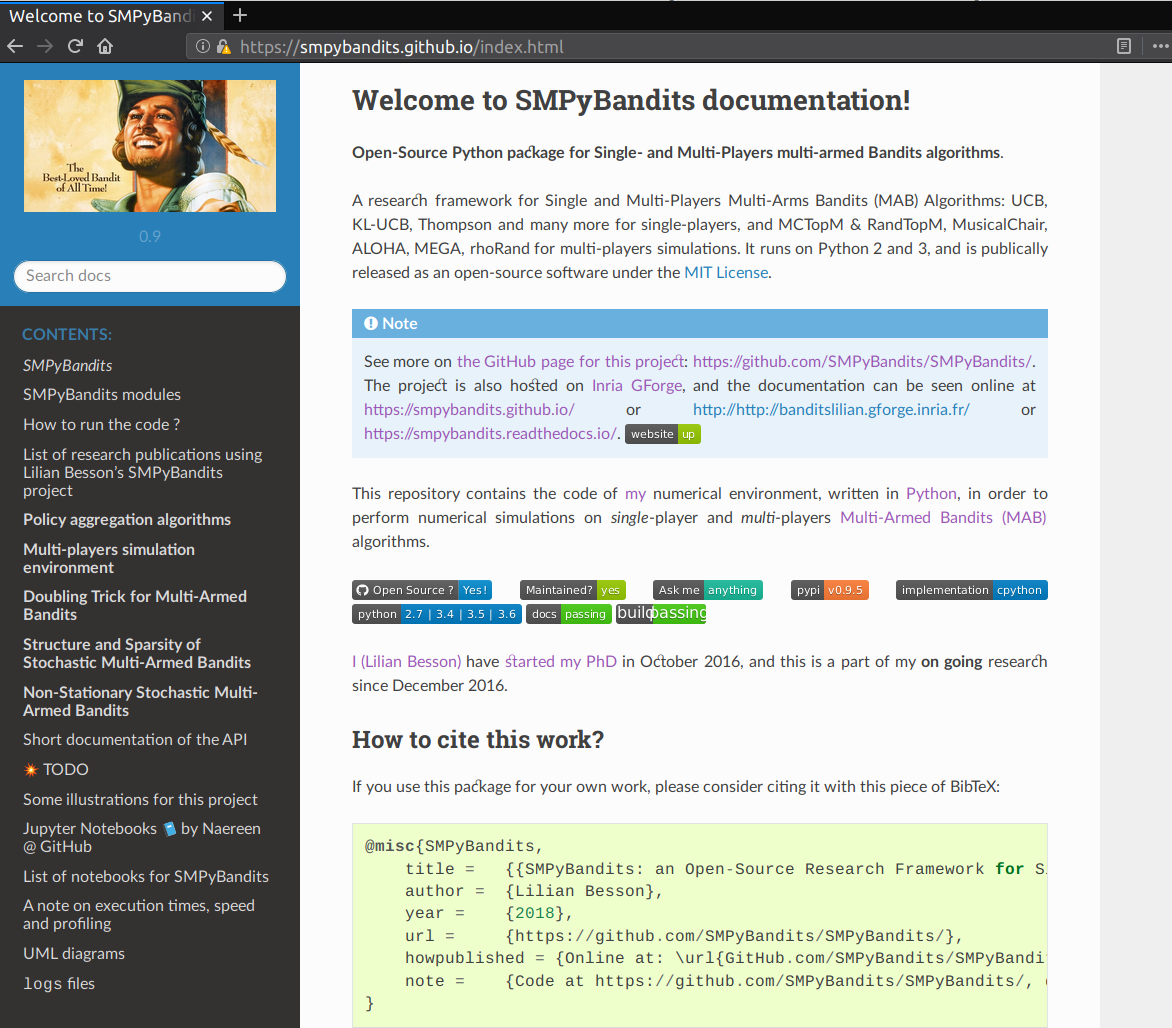
\includegraphics[width=0.495\linewidth]{overview_documentation_1.png}
    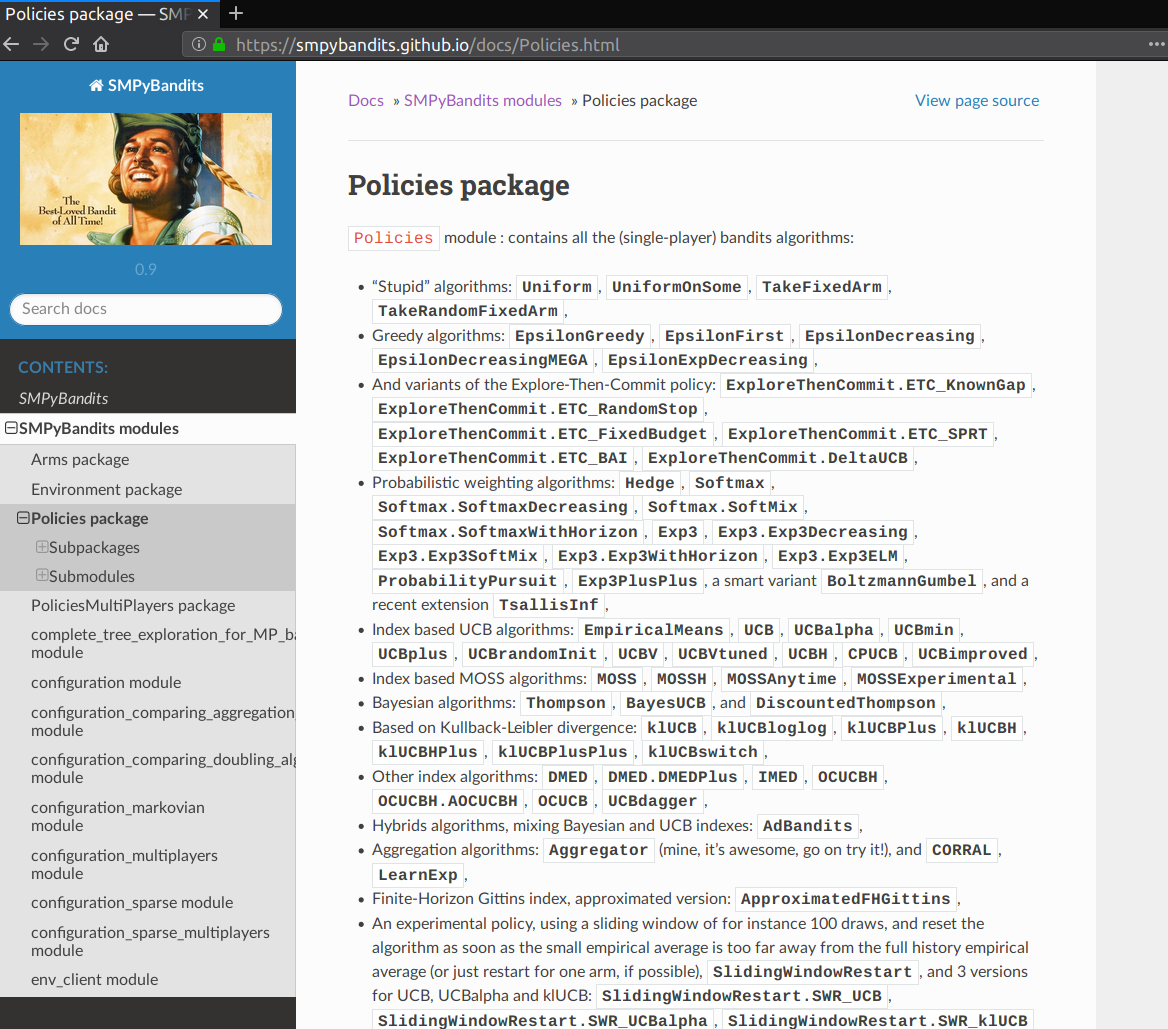
\includegraphics[width=0.495\linewidth]{overview_documentation_2.png}
	\caption{Screenshots from two pages of the documentation: the homepage (\texttt{\href{https://SMPyBandits.GitHub.io}{SMPyBandits.GitHub.io}}), and a list of all the algorithms in the \texttt{Policies} module.}
	\label{fig:3:twoScreenshotsOfTheDocumentation}
\end{figure}

\begin{figure}[h!]  % [htbp]
    \centering
	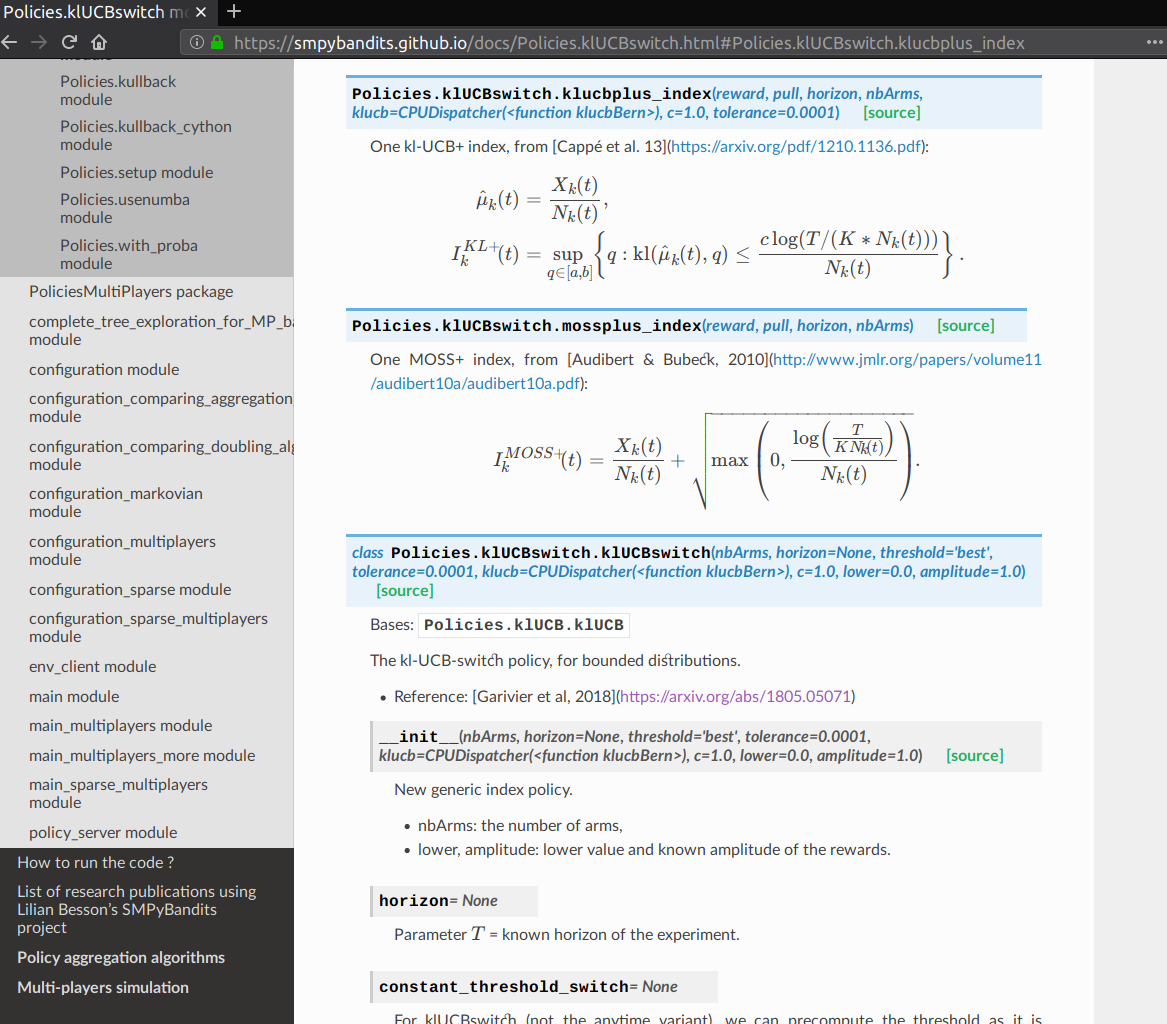
\includegraphics[width=0.495\linewidth]{overview_documentation_3.png}
	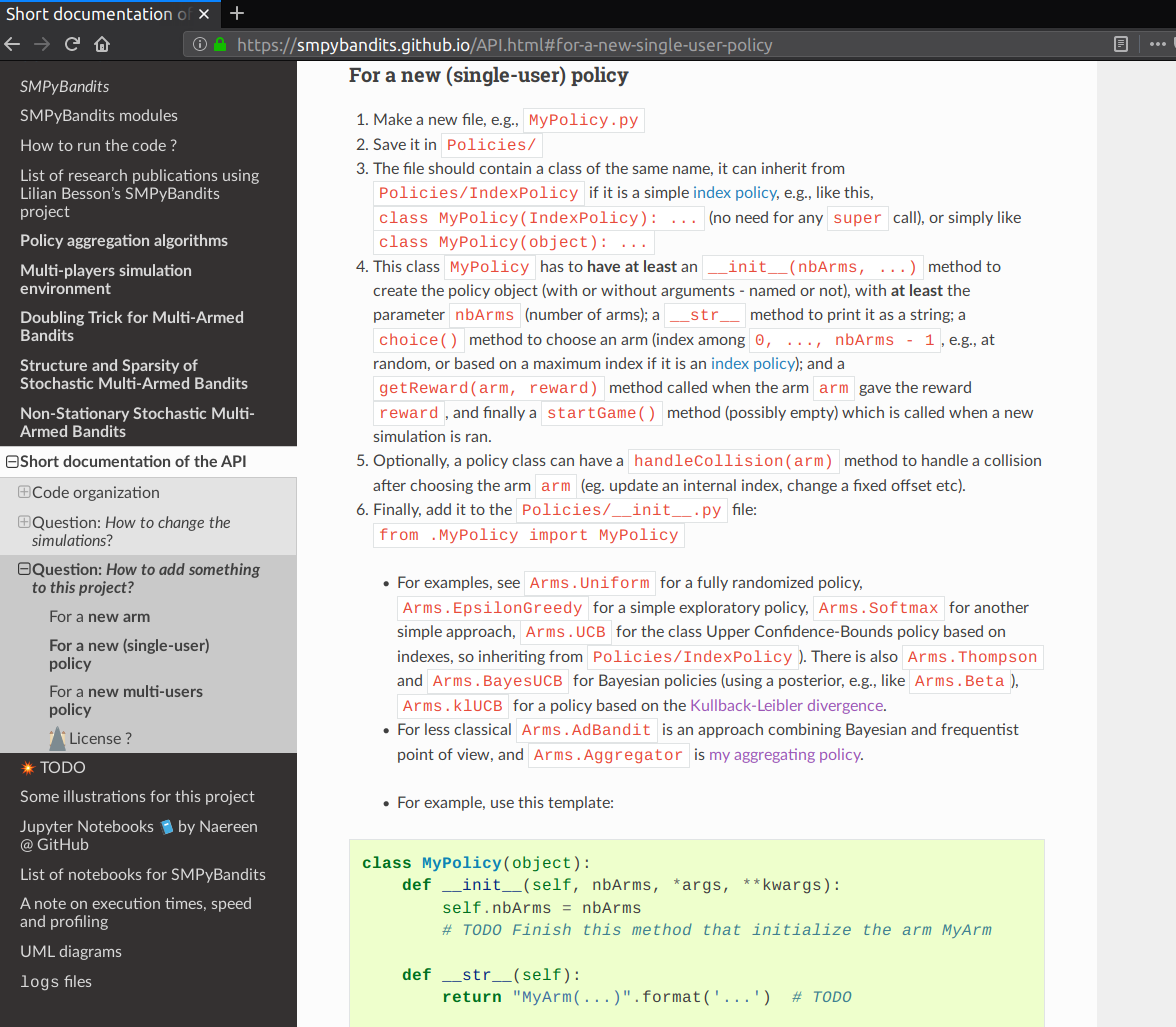
\includegraphics[width=0.495\linewidth]{overview_documentation_4.png}
	\caption{Screenshots from two other pages of the documentation: the \texttt{klUCBSwitch} policy, and details of the code organization, to know how to add a new policy.}
	\label{fig:3:twoMoreScreenshotsOfTheDocumentation}
\end{figure}


\subsection{How to run experiments?}

We show how to install SMPyBandits, and an example of how to run a simple experiment.
See this page \texttt{\href{https://SMPyBandits.GitHub.io/How_to_run_the_code.html}{SMPyBandits.GitHub.io/How\_to\_run\_the\_code.html}} for more details.
SMPyBandits is also available on Pypi, see \texttt{\href{https://pypi.org/project/SMPyBandits/}{pypi.org/project/SMPyBandits}}, you can install it directly with \texttt{sudo pip install SMPyBandits}, or from a \texttt{virtualenv} \cite{virtualenv}.
This bash code shows how to clone the code, and install the requirements for Python 3 (once):

% https://tex.stackexchange.com/a/12430/
\begin{small}
    \begin{listing}[h!]
        \begin{minted}[linenos=true,numbersep=5pt,frame=lines,framesep=2mm]{bash}
# 1. get the code in the folder you want
$ git clone https://GitHub.com/SMPyBandits/SMPyBandits.git
$ cd SMPyBandits.git
# 2. install the requirements
$ pip install -r requirements.txt
        \end{minted}
        \caption{Example of Bash code to download and install dependencies of SMPyBandits.}
        % \captionof{listing}{Small snippet of Bash code to download and install dependencies of SMPyBandits \label{lst:3:howToInstallLibrary}.}
        \label{lst:3:howToInstallLibrary}
    \end{listing}
\end{small}

Simulations are easily executed, \eg, Code~\ref{lst:3:howToRunBasicLibrary} shows how to start $N=1000$ repetitions of a simple non-Bayesian Bernoulli-distributed problem, for $K=9$ arms, an horizon of $T=10000$ and on $4$ CPU.
It takes about $20$ min, on a $4$-core $64$-bit GNU/Linux laptop.
Environment variables (\texttt{N=1000} etc) in the command line are not required, but they are convenient.

% https://tex.stackexchange.com/a/12430/
\begin{small}
\begin{listing}[h!]
    \begin{minted}[linenos=true,numbersep=5pt,frame=lines,framesep=2mm]{bash}
# 3. run a single-player simulation
$ BAYES=False ARM_TYPE=Bernoulli N=1000 T=10000 K=9 N_JOBS=4 \
  MEANS=[0.1,0.2,0.3,0.4,0.5,0.6,0.7,0.8,0.9] \
  python3 main.py configuration.py
    \end{minted}
    \caption{Example of Bash code to run a simple experiment with SMPyBandits.}
    % \captionof{listing}{Small snippet of Bash code to run a simple experiment with SMPyBandits \label{lst:3:howToRunBasicLibrary}.}
    \label{lst:3:howToRunBasicLibrary}
\end{listing}
\end{small}


\subsection{Example of a simulation and illustration}

A small script \texttt{configuration.py}
% (\texttt{\href{https://SMPyBandits.GitHub.io/docs/configuration.html}{SMPyBandits.GitHub.io/docs/configuration.html}})
is used to import the arm classes (\texttt{\href{https://SMPyBandits.GitHub.io/docs/Arms.html}{Arms}} module), the policy classes (\texttt{\href{https://SMPyBandits.GitHub.io/docs/Policies.html}{Policies}} module) and define the problems and the experiments.
Choosing the algorithms to include is done by changing
the \texttt{configuration["policies"]} list in the \texttt{configuration.py} file.
For instance, one can compare the standard anytime \klUCB{} algorithm (class \texttt{\href{https://SMPyBandits.GitHub.io/docs/Policies.klUCB.html}{klUCB}} in \texttt{Policies} module) against the non-anytime variant $\klUCB^{++}$ algorithm (\texttt{\href{https://SMPyBandits.GitHub.io/docs/Policies.klUCBPlusPlus.html}{klUCBPlusPlus}}), and also \UCB{} with $\alpha=1$ (\texttt{\href{https://SMPyBandits.GitHub.io/docs/Policies.UCBalpha.html}{UCB}}) and Thompson sampling (\texttt{\href{https://SMPyBandits.GitHub.io/docs/Policies.Thompson.html}{Thompson}}) with a Beta posterior (\texttt{\href{https://SMPyBandits.GitHub.io/docs/Policies.Posterior.Beta.html}{Posterior.Beta}})).

% https://tex.stackexchange.com/a/12430/
\begin{small}
\begin{listing}[h!]
    \begin{minted}[linenos=true,numbersep=5pt,frame=lines,framesep=2mm]{python3}
configuration["policies"] = [
    { "archtype": klUCB, "params": { "klucb": klucbBern } },
    { "archtype": klUCBPlusPlus, "params": {"horizon": T, "klucb": klucbBern}},
    { "archtype": UCBalpha, "params": { "alpha": 1 } },
    { "archtype": Thompson, "params": { "posterior": Beta } }
]
    \end{minted}
    \caption{Example of Python code to configure the list of algorithms tested on a problem.}
    % \captionof{listing}{Small snippet of Python code to configure the list of algorithms tested on a problem. \label{lst:3:howToConfigureAlgorithms}.}
    \label{lst:3:howToConfigureAlgorithms}
\end{listing}
\end{small}

\begin{figure}[h!]  % [htbp]
	\centering
	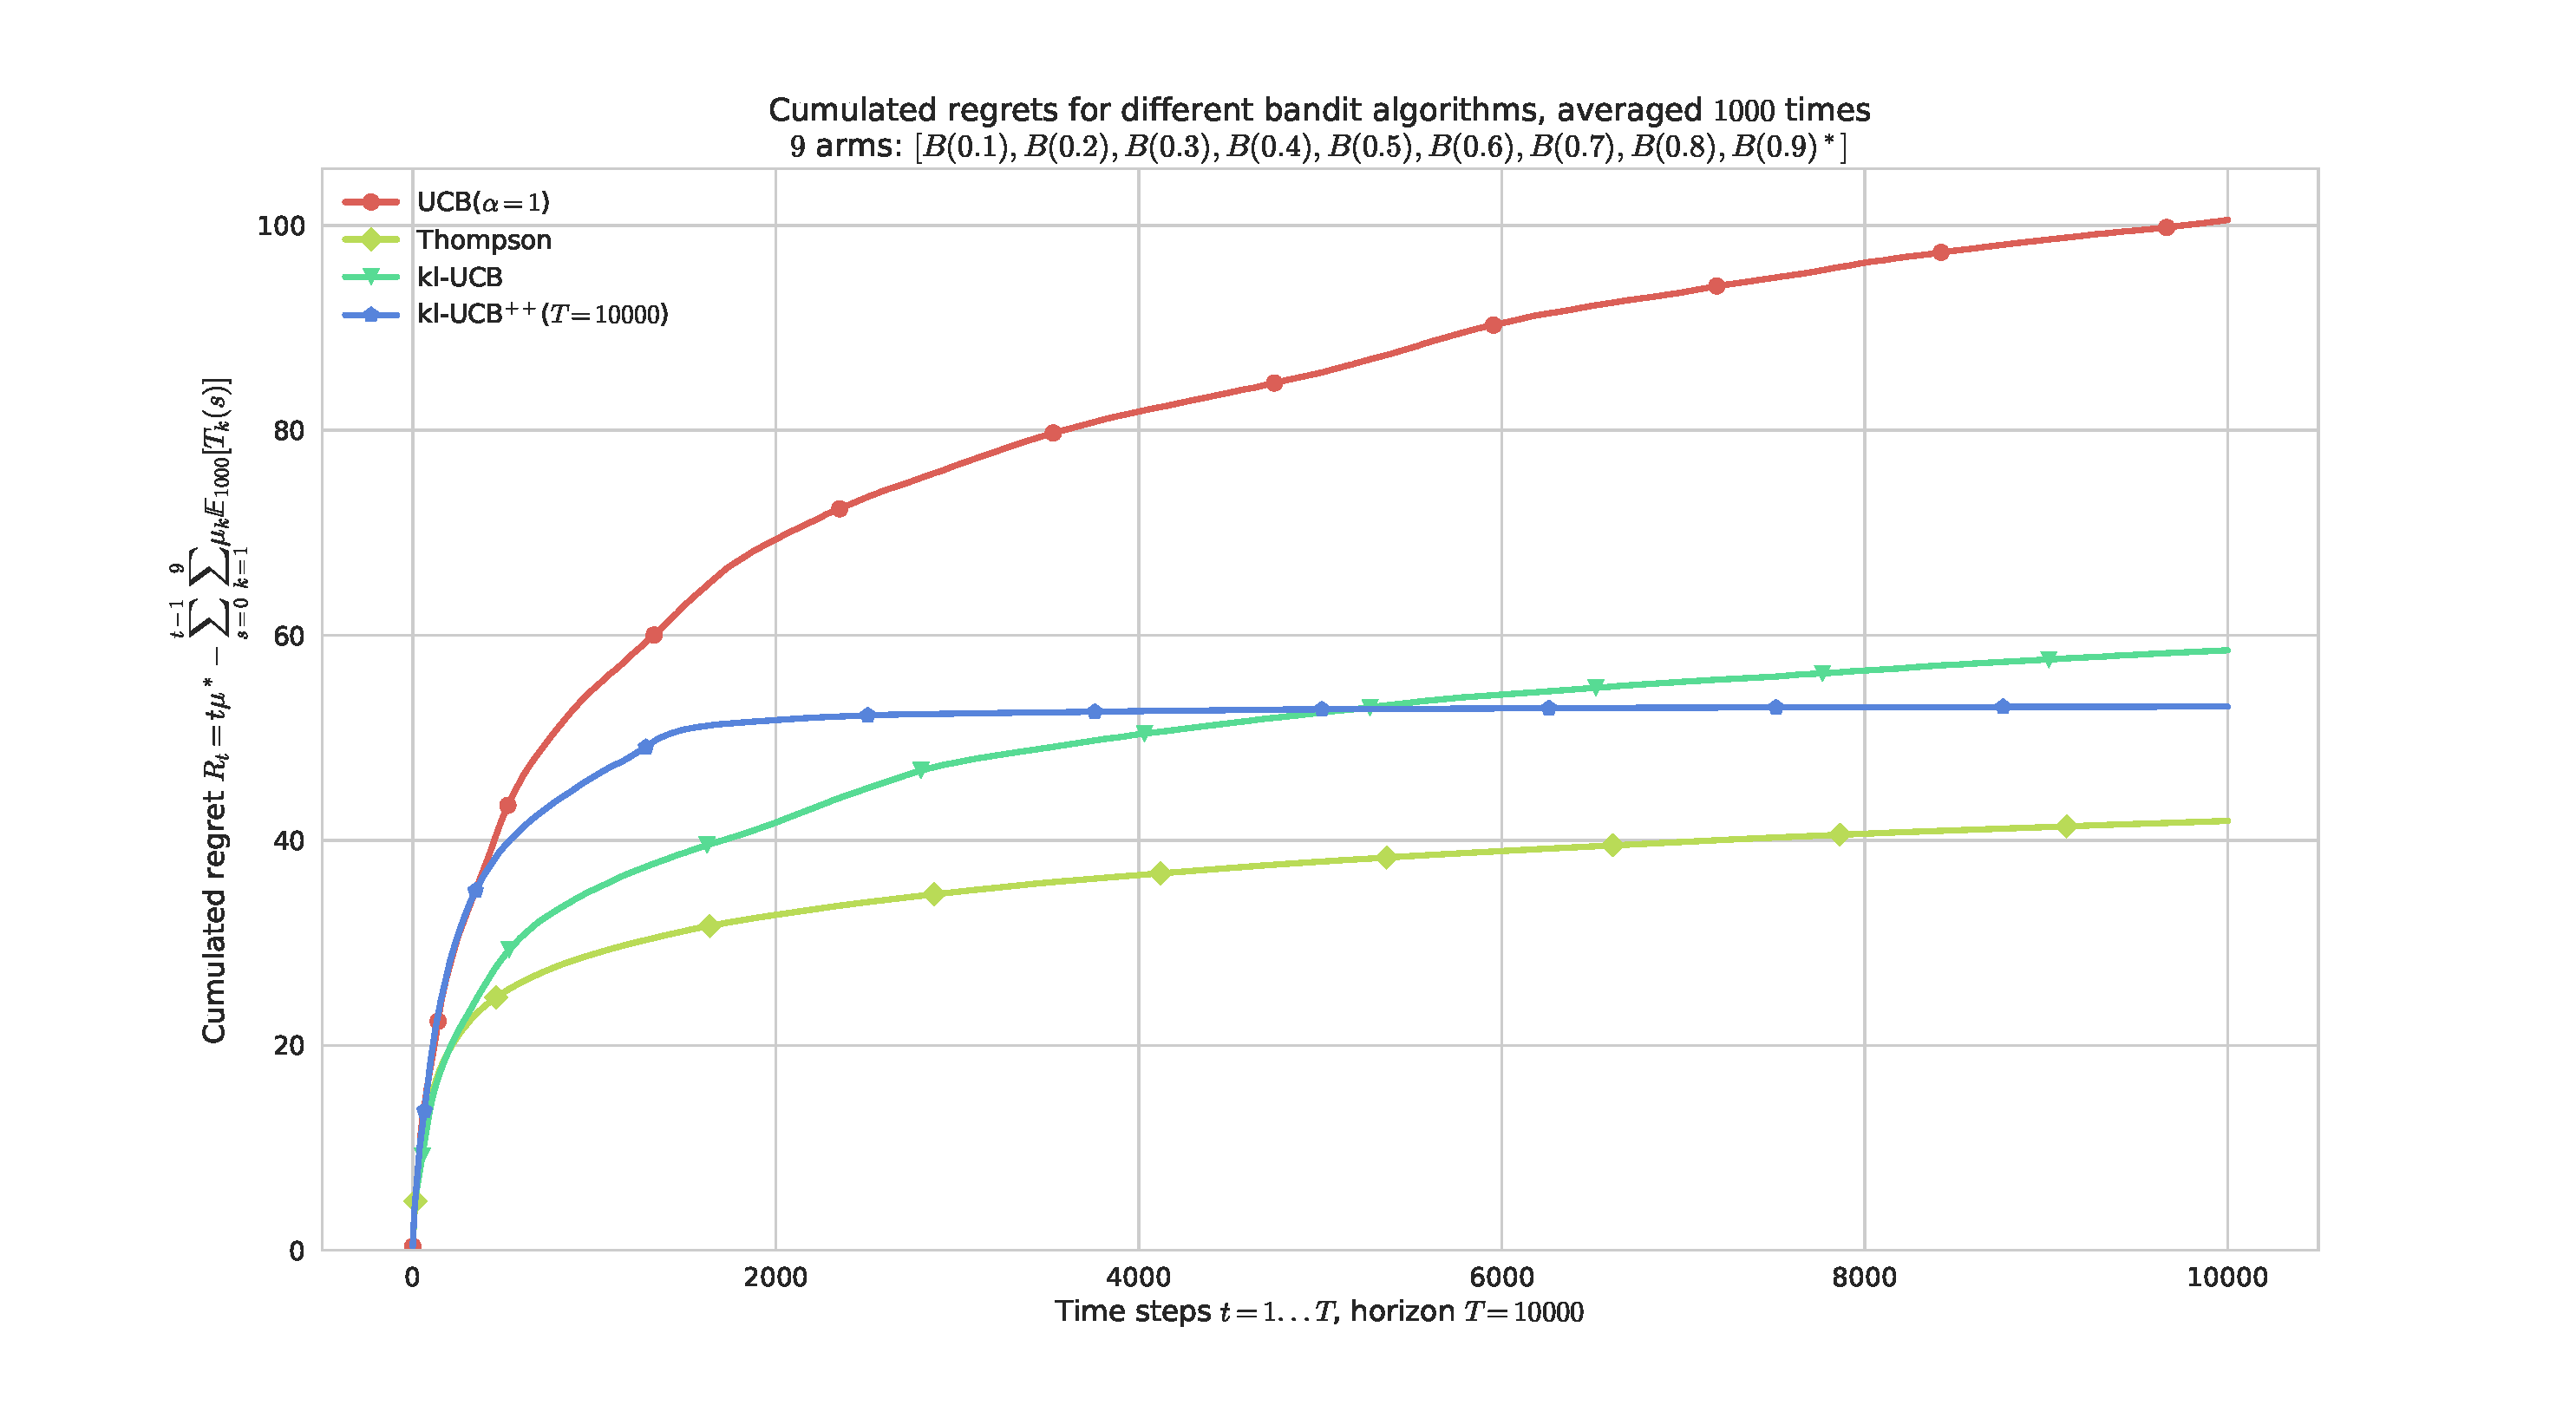
\includegraphics[width=1.05\linewidth]{3.pdf}
	\caption[Example of a single-player simulation showing the average regret of $4$ algorithms.]{
		Example of a single-player simulation showing the average regret of four algorithms (\textcolor{red}{\UCB}, \textcolor{blue}{\KLUCBpp}, \textcolor{darkgreen}{\klUCB} and \textcolor{gold}{Thompson sampling}). They all perform very well: each algorithm is known to be order-optimal (\ie, its regret is proven to match the lower-bound up-to a constant), and each but UCB is known to be asymptotically optimal (\ie, with the constant matching the lower-bound).
	}
	\label{fig:3:firstPlot}
\end{figure}

Running the simulation as shown above will save figures in a sub-folder, as well as save data (pulls, rewards, regret and other data) in a HDF5 file\footnote{~For example, this simulation produced this HDF5 file\\\texttt{\href{https://github.com/SMPyBandits/SMPyBandits/blob/master/plots/paper/example.hdf5}{GitHub.com/SMPyBandits/SMPyBandits/blob/master/plots/paper/example.hdf5}}}
\cite{h5py}.
% \texttt{\href{http://docs.h5py.org/en/stable/high/file.html}{docs.h5py.org/en/stable/high/file.html}}).
Figure~\ref{fig:3:firstPlot} above shows the average regret for these $4$ algorithms.
% The regret is the difference between the cumulated rewards of the best fixed-armed strategy (which is the oracle strategy for stationary bandits), and the cumulated rewards of the considered algorithms.
The Figure~\ref{fig:3:firstPlot_hist} below shows the histogram of regret obtained at the end of the experiment (\ie, $R_T$) for the same example.

\begin{figure}[h!]  % [htbp]
	\centering
	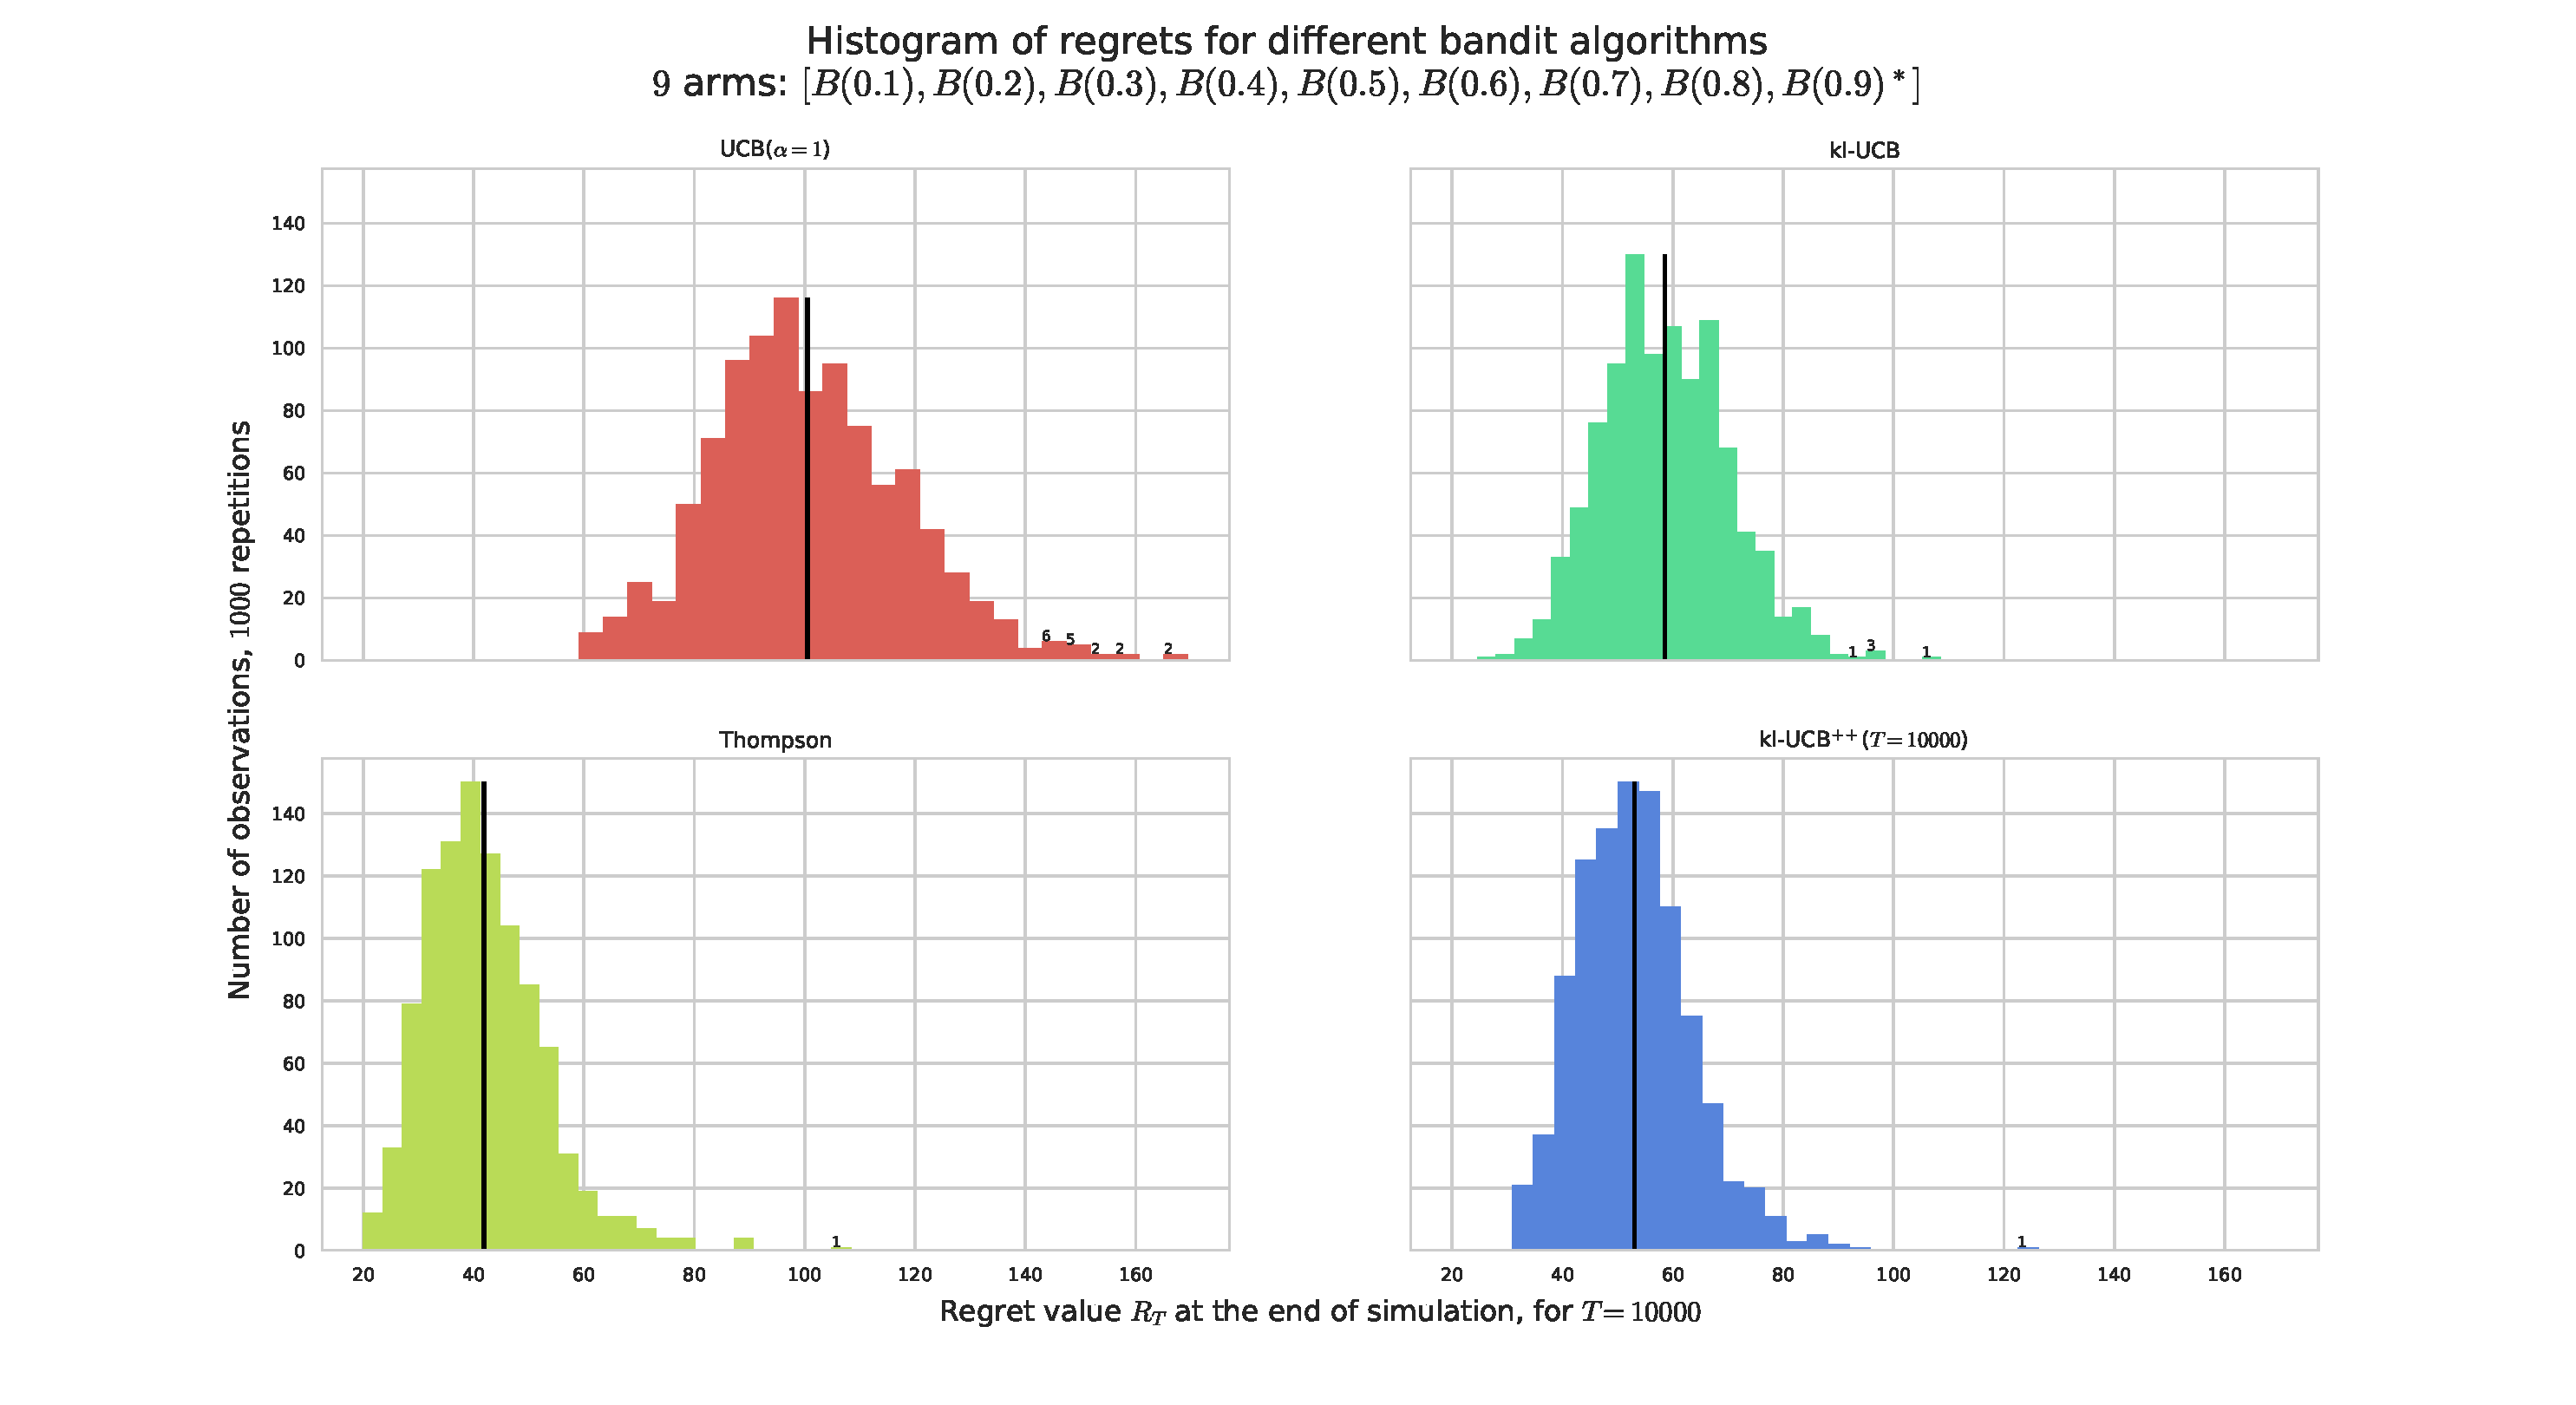
\includegraphics[width=1.05\linewidth]{3_hist.pdf}
	\caption{Histogram of regret for the same experiment as of Figure~\ref{fig:3:firstPlot}. For instance, \textcolor{gold}{Thomson sampling} is very efficient in average (\textcolor{gold}{in yellow}), and \textcolor{red}{\UCB} shows a larger variance (\textcolor{red}{in red}).}
	\label{fig:3:firstPlot_hist}
\end{figure}


\subsection{Dependencies on other Python libraries}
\label{sub:3:dependencies}

This library is written in Python \cite{python}, for versions 2.7+ or 3.4+, using \texttt{matplotlib} \cite{matplotlib} for 2D plotting, \texttt{numpy} \cite{numpy} for data storing, random number generations and operations on arrays, \texttt{scipy} \cite{scipy} for statistical and special functions, and \texttt{seaborn} \cite{seaborn} for clean plotting and colorblind-aware colormaps.

Optional dependencies include \texttt{joblib} \cite{joblib} for parallel simulations, \texttt{numba} \cite{numba} for automatic speed-up on small functions (using a Just-in-Time compiler), \texttt{sphinx} \cite{sphinx} for generating the documentation, \texttt{virtualenv} \cite{virtualenv} for launching simulations in isolated environments, and \texttt{jupyter} \cite{jupyter} used with \texttt{ipython} \cite{ipython} to experiment with the code.

All the quoted libraries are free and open-source and can be installed in one command using the \texttt{pip} (\texttt{\href{https://pip.pypa.io/}{pip.PyPa.io}}) or \texttt{conda} (\texttt{\href{http://conda.anaconda.org/}{conda.anaconda.org}}) package manager.
%
When SMPyBandits is installed using \texttt{pip install SMPyBandits}, the dependencies are of course automatically installed if not already present.


\subsection{Continuous integration with Read the Docs and Travis CI}

Since $2017$ and $2018$, SMPyBandits is using two online continuous integration (CI) services, to automatically build and host its documentation, and to automatically test the library on some numerical simulations.
%
These CI services are free for open-source works, and are both triggered whenever a modification of the codebase is sent to the hosting platform GitHub.

\textbf{Read the Docs.}
Since $2017$, we have been using the free web service provided by Read the Docs (\href{https://readthedocs.org/}{\texttt{ReadTheDocs.org}}).
Read the Docs allows to automatically build the documentation after every commit. This allows to regularly check that the library is well formatted and can be imported correctly, as well as keeping the online documentation up-to-date.
Moreover, they offer to host the documentation online, at \href{https://smpybandits.rtfd.io/}{\texttt{SMPyBandits.ReadTheDocs.io}}.
For more details, see \href{https://readthedocs.org/projects/smpybandits/}{\texttt{ReadTheDocs.org/projects/SMPyBandits}}.
%
Since its first use, the service did about 180 builds, and about $10\%$ of them were useful to detect newly introduced issues or bugs in the code.
The build is configured using the \texttt{.readthedocs.yml} file in SMPyBandits main folder, and it builds the documentation in about two minutes.
I have also been building the documentation manually on a weekly basis, to also host it on \href{https://smpybandits.github.io/}{\texttt{SMPyBandits.GitHub.io}} thanks to GitHub pages.
In the last two years, the documentation saw about 11000 unique visits, while the GitHub project have been visited about 4500 unique visits.


\textbf{Travis CI.}
Since $2018$, we use the free web service provided by Travis CI (\href{https://travis-ci.org/}{\texttt{Travis-CI.org}}).
It allows to automatically run short numerical simulations after every commit,
in order to check that each modification on any part of the codebase does not break anything, as well as giving an up-to-date example of log files that shows online the results of different examples of experiments. The tests covers all the main models and almost all the algorithms implemented in SMPyBandits, and it has been proven very useful to quickly find and fix new bugs.
For more details, see \href{https://travis-ci.org/SMPyBandits/SMPyBandits}{\texttt{Travis-CI.org/SMPyBandits/SMPyBandits}}.
%
Since its first use, the service did about $190$ builds, and about $30\%$ of them were useful to detect newly introduced issues or bugs in the code.
The build is configured using the \texttt{.travis.yml} file in SMPyBandits main folder, and it runs numerical experiments with a short horizon (\eg, $T=100$) and a small number of repetitions (\ie, $N=4$), but covering all the different models implemented by SMPyBandits (and even including some that are not covered in this chapter, like the Markov model, or the sparse multi-players model).
Builds typically run for $15$ minutes, and Travis CI have been proven to be very useful in our development process.



\subsection{List of research works using SMPyBandits}
\label{sub:3:listResearchWorksUsingSMPyBandits}

SMPyBandits has been used for the following research articles since $2017$, and it is used for the previous and the next chapters of this thesis (except in Chapter~\ref{chapter:4}).
%
We give a link to a page on the documentation, that gives detailed instructions to reproduce the results presented in this research paper, details about the models and the notations, and bibliographic references.

\begin{itemize}
    \item
In \cite{Besson2018WCNC} and in Chapter~\ref{chapter:2} above, we used SMPyBandits to illustrate and compare different aggregation algorithms. We designed a variant of the Exp4 algorithm for online aggregation of experts \cite{Bubeck12}, called \texttt{\href{https://SMPyBandits.GitHub.io/docs/Policies.Aggregator.html}{Aggregator}}.
The documentation page is on \texttt{\href{https://SMPyBandits.GitHub.io/Aggregation.html}{SMPyBandits.GitHub.io/Aggregation.html}}
% Aggregating experts is a well-studied idea in sequential learning and in machine learning in general. We showed that it can be used in practice to select on the run the best bandit algorithm for a certain problem from a fixed pool of experts. This idea and algorithm can have interesting impact for Opportunistic Spectrum Access applications \cite{Jouini09} that use multi-armed bandits algorithms for sequential learning and network efficiency optimization.

    \item
In \cite{Besson2018ALT} and in Chapter~\ref{chapter:5} below, we used SMPyBandits for all the simulations for multi-players bandit algorithms. We designed the two \texttt{\href{https://SMPyBandits.GitHub.io/docs/PoliciesMultiPlayers.RandTopM.html}{RandTopM}} and \texttt{\href{https://SMPyBandits.GitHub.io/docs/PoliciesMultiPlayers.MCTopM.html}{MCTopM}} algorithms and proved than they obtain logarithmic regret in the usual setting, and outperform significantly the previous state-of-the-art solutions (\ie, \texttt{\href{https://SMPyBandits.GitHub.io/docs/PoliciesMultiPlayers.rhoRand.html}{rhoRand}}, \texttt{\href{https://SMPyBandits.GitHub.io/docs/Policies.MEGA.html}{MEGA}} and \texttt{\href{https://SMPyBandits.GitHub.io/docs/Policies.MusicalChair.html}{MusicalChair}}).
Similarly, see the page \texttt{\href{https://SMPyBandits.GitHub.io/MultiPlayers.html}{SMPyBandits.GitHub.io/MultiPlayers.html}}

    \item
In \cite{Besson2018DoublingTricks} (see Appendix~\ref{app:2:DoublingTricks}), we used SMPyBandits to illustrate and compare different "doubling trick" schemes.
\texttt{\href{https://SMPyBandits.GitHub.io/DoublingTrick.html}{SMPyBandits.GitHub.io/DoublingTrick.html}}
% In sequential learning, an algorithm is said to be ``anytime'' if it does not need to know the horizon $T$ of the experiments. A well-known trick for transforming any ``non-anytime'' algorithm to an ``anytime'' variant is the ``Doubling Trick'': start with an horizon $T_0\in\mathbb{N}^*$, and when $t > T_i$, use $T_{i+1} = 2 T_i$. We studied two generic sequences of growing horizons (geometric and exponential), and we proved two theorems that generalized previous results. A geometric sequence suffices to keep minimax regret bounds (in $R_T = \mathcal{O}(\sqrt{T})$), with a constant multiplicative loss $\ell \leq 4$, but cannot be used to keep a logarithmic regret bound (in $R_T = \mathcal{O}(\log(T))$). And an exponential sequence can be used to keep logarithmic bounds, with a constant multiplicative loss also $\ell \leq 4$ in the usual setting. It is still an open question to know if a well-tuned exponential sequence can keep minimax bounds, or "weak" minimax bounds (in $R_T = \mathcal{O}(\sqrt{T \log(T)})$).

    \item
In \cite{Besson2019GLRT} and \cite{Besson2019Gretsi}, and in Chapter~\ref{chapter:6} below, we used SMPyBandits for piece-wise stationary MAB models (only for the single-player case). We illustrate and compare different algorithms designed for this family of non-stationary problems.
We designed the \texttt{\href{https://SMPyBandits.GitHub.io/docs/Policies.GLR_UCB.html}{GLRklUCB}} policy, and implemented most of the state-of-the-art passive or active adaptive policies, both adversarial- or stochastic-based, designed to tackle the piece-wise stationary MAB problems.
We also implemented a large benchmark of different piece-wise stationary problems.
See \texttt{\href{https://SMPyBandits.GitHub.io/NonStationary.html}{SMPyBandits.GitHub.io/NonStationary.html}}
\end{itemize}


% ----------------------------------------------------------------------------
\section{Experimental comparisons of state-of-the-art algorithms}
\label{sec:3:reviewSPAlgorithms}

% \TODOL{Write text for this Section, write configuration.py file, run short-term experiment, include them, if happy about it, run longer ang larger experiments}

In this section, we use the SMPyBandits library to compare experimentally various state-of-the-art (single-player) algorithms on some MAB problems.
We first detail the list of different algorithms that we compare.
% , and the different problems on which they are all tested.
We then give the results of the numerical experiments, in terms of mean regret at the end of the experiment of different horizons $T$.
Additional results in terms of real measurements of time and memory are given and discussed in the next Section~\ref{sec:3:timeAndMemoryCosts}.
% %
% Finally, we give some observations on the results, and the main take-away message of this section is the following: in all the rest of this thesis, we focus on two algorithms depending if simplicity or efficiency is favored:
% \begin{itemize}
%     \item
%     \UCB{} is used in the more applied Chapter~\ref{chapter:4}, when simplicity is favored,
%     \item
%     \klUCB{} is used, in the two more theoretical Chapters~\ref{chapter:5} and \ref{chapter:6}, when efficiency is favored.
% \end{itemize}


\subsection{Experimental setup: algorithms and problems}

% \paragraph{List of algorithms.}

We consider the $9$ following algorithms, and $7$ more are described in Appendix~\ref{sub:3:additionalExperiments}.
For each of them, we give a bibliographic reference, that corresponds to a recent article studying it and not the first one which introduced it.
We give the chosen tuning of its parameters, for parametric algorithms.
Algorithms that are ``not anytime'' use the exact value of the horizon $T$, and when increasing values of $T$ are studied for the same problem, they use the correct successive values.
%
For reproducibility, we also give in ``\texttt{typewriter font}'' the name of the corresponding class in the \texttt{Policies} module in SMPyBandits
(\eg, $\UCB_1$ is \texttt{Policies.UCBalpha}).

\begin{enumerate}
    \item
    %  Algorithm 1 is
    $\varepsilon$-greedy \cite{Bubeck12} (\texttt{EpsilonDecreasing}),
    % shown in Algorithm~\ref{algo:2:naiveStrategies} above,
    using $\varepsilon_t = \varepsilon_0 / t$, and $\varepsilon_0 = 0.1$ (chosen arbitrarily).
    It has a very small cost in terms of time and memory, but it usually achieves linear regret in practice, despite of the theoretical regret bound.

    \item
    %  Algorithm 2 is
    Explore-then-Commit \cite{GarivierETC2016} (\texttt{ETC\_KnownGap}),
    % shown in Algorithm~\ref{algo:2:naiveStrategies} above,
    that knows the horizon, and a lower-bound on the gap between arms (chosen arbitrarily as $\delta=0.01$, valid for all problems).
    Similarly to $\varepsilon$-greedy, it has a very small footprint in terms of time and memory, but most of the times it only obtains large (linear) regret.

    \item
    %  Algorithm 3 is
    $\mathrm{Exp}3^{++}$ from \cite{Seldin17} (\texttt{Exp3PlusPlus}), using $\alpha=3$ and $\beta=256$ as advised.
    It is a recent anytime variant of the $\mathrm{Exp3}$ algorithm, which was proven to obtain good ``best of both world'' performances.
    % meaning that it achieves $\cO(K\log(T)/\Delta^2)$ regret for problem-dependent bounds, and $\cO(\sqrt{KT})$ for problem-independent bounds.

    \item
    %  Algorithm 4 is
    $\UCB_1$ from \cite{Auer02} (\texttt{UCBalpha}), shown in Algorithm~\ref{algo:2:indexPolicy} above, using $\alpha=1$.
    It achieves order-optimal problem-dependent bounds with a $\cO(K\log(T)/\Delta^2)$ regret.

    \item
    %  Algorithm 5 is
    \klUCB{} from \cite{KLUCBJournal} (\texttt{klUCB}), also shown in Algorithm~\ref{algo:2:indexPolicy} above, using the Bernoulli KL divergence and the corresponding \klUCB{} indexes (coded as \texttt{kullback.klucbBern}).
    % It achieves asymptotical optimal problem-dependent bounds with a $\cO(\log(T))$ regret.
    % with the scaling factor matching Lai and Robbins' lower-bound \cite{LaiRobbins85}.
    It is computationally more costly that \UCB, as at each time step $t$ and for each arm $k$, a convex optimization problem must be solved approximately, in order to compute the $K$ indexes.
    In practice, a few steps of a simple bisection search method are enough to obtain a good numerical precision, and empirically we found that even in the worst cases \klUCB{} is no more than one order of magnitude slower than \UCB.
    % of more than 10 digits
    % \TODOL{Si on en pas parlé avant, ou après dans une annexe, je peux dire un mot ici à propos de l'implémentation en Cython ou en C des fonctions kl et indices kl-UCB !}

    \item
    %  Algorithm 6 is
    Thompson sampling from \cite{Kaufmann12Thompson} (\texttt{Thompson}), using a Beta prior and posterior, initially uniform (\ie, $\pi_k(0)=\mathrm{Beta}(1,1)$).
    % It was also proven to achieve asymptotical optimal problem-dependent bounds \cite{Kaufmann12Thompson,AgrawalGoyal11}.
    It is efficient in terms of storage, and even if $K$ random samples must be sampled from the arms posteriors at each time step $t$, Thompson sampling is not much slower than \UCB, if the random number generator used for the simulations is efficient (it is the case for SMPyBandits, as we use \texttt{numpy.random} module which relies on highly optimized C or Cython code).

    \item
    %  Algorithm 7 is
    Bayes-UCB from \cite{Kaufmann12BUCB} (\texttt{BayesUCB}), using a Beta prior and posterior, initially uniform, \ie, $\pi_k(0)=\mathrm{Beta}(1,1)$.
    % It was also proven to achieve asymptotical optimal problem-dependent bounds \cite{Kaufmann12BUCB}.
    It is comparable to Thompson sampling in terms of memory complexity, but slower as computing a quantile is more costly than sampling from a distribution.
    But in particular for Bernoulli distributed arms and for Beta posteriors and priors, Bayes-UCB is only about twice as slow as Thompson sampling.

    \item
    %  Algorithm 8 is
    AdBandits from \cite{Truzzi13} (\texttt{AdBandits}), using $\alpha=1$.
    % It follows the same assumptions as Thompson sampling and Bayes-UCB, and uses a Beta posterior on each arm. It uses a random mixture between the two algorithms, and with a certain probability it uses the Thompson decision rule (\ie, choose the arm maximizing one draw of random samples from the posteriors), otherwise it uses the Bayes-UCB decision rule (\ie, choose the arm maximizing the $1-1/t$ quantile).
    % It was proposed in this article \cite{Truzzi13} and illustrated on empirical simulations, but no theoretical analysis was given, and it did not gain popularity since then.
    In practice, it is usually (slightly) more efficient than both Thompson sampling and Bayes-UCB in terms of regret, it is comparable in terms of computation times, but costs more memory.

    \item
    %  Algorithm 9 is
    BESA (Best Empirical Sampled Average) from \cite{Baransi2014},
    % , and it consists in trying to fix a simple observation.
    % For instance in \UCB, if arm $1$ has $100$ samples and arm $2$ has $50$ samples, it should make more sense to only use $50$ samples of arm $1$ to compute and compare any statistics for each arm (\eg, mean).
    % The BESA algorithm for $K=2$ arms is then very simple: at each time step, if arms $1$ and $2$ have $n_1$ and $n_2$ samples, and if $n_1>n_2$ (for instance), first it sub-samples $n_2$ observations from $n_1$, then it computes the mean of these observations, and play the arm maximizing this mean (now that there is the same number of observations for both arms, it makes more sense to compare these quantities).
    % It was analyzed partially for the two-armed case, and the authors illustrated that it can be very efficient empirically.
    % Analyzing it in the generic case was found to be difficult, and is still an open problem.
    which is implemented with a binary tournament, written in a naive but efficient way
    (\ie, not using recursive functions, by using the \texttt{BESA} class with the \texttt{''non\_recursive''=True} option).
    But the extension to $K>2$ arms is still costly in terms of both time and memory, as illustrated below, and blows-up exponentially  when $K$ increases.
\end{enumerate}

We focused here on the most well known algorithms, discussed in Section~\ref{sec:2:famousMABalgorithms}, and two others that are efficient but less known (AdBandits and BESA).
To highlight that SMPyBandits implements many other MAB algorithms proposed in recent works, we detail in Appendix~\ref{sub:3:additionalExperiments} $7$ other algorithms.
They are more recent (\eg, $3$ from $2018$ and $2$ from $2019$) and are usually more complex, or based on a different point-of-view.
The numerical results presented below include these extra algorithms, to justify empirically that despite their respective qualities, and despite being very efficient, it is reasonable to focus on \UCB{} and \klUCB{} in the rest of this thesis, as they stay comparable with or more efficient than other recent algorithms, but are simpler to implement (\eg, when comparing \UCB{} to \texttt{ApproximatedFHGittins} or $\mathrm{MOSS}$-$\mathrm{Anytime}$) to manipulate theoretically (\eg, when comparing \klUCB{} to BESA, PHE or RCB).


\paragraph{Randomly sampled problems.}
%
For brevity, we prefer to focus on a single kind of distributions (Bernoulli),
but similar results were observed for other distributions, in particular for (possibly truncated) Gaussian distributions.
%
% % \begin{itemize}
%     % \item
%     \textbf{Problem 1} considers $K$ arms of equally spaced means, in $[0,1]$.
%     It uses a minimum mean of $0.05$ and a maximum mean of $0.95$.
%     For instance, for $K=2$, $\bm{\mu}=[0.05, 0.95]$ and for $K=5$, $\bm{\mu} = [0.05, 0.275, 0.5, 0.725, 0.95]$.

%     % \item
% \textbf{Problem 2} takes another approach.
For a fixed number of arms $K \geq 2$,
instead of simulating a large number of times the same problem,
we generate a new random problem for each independent run.
%
We consider a randomly generated vector of means, each being sampled uniformly at random in $[0,1]$, with a minimum gap of $\Delta^{\min}$, as well as minimum and maximum values of $\mu_{\min}$ and $\mu_{\max}$, that is denoted by $\bm{\mu} \sim \cE(\Delta^{\min},\mu_{\min},\mu_{\max})$.
This space $\cE_{\Delta^{\min}}$ is defined as $\{ \bm{\mu} \in [\mu_{\min}, \mu_{\max}]^K : \min_{k\neq k'} |\mu_k - \mu_{k'}| \geq \Delta^{\min} \}$.
We use $\mu_{\min} = \Delta^{\min}$ and $\mu_{\max} = 1 - \Delta^{\min}$,
and the value used for $\Delta^{\min}$ is $0.1$ for $K \leq 3$ (for ``easy'' problems), and $\frac{1}{3 K}$ for $K \geq 5$ (for ``harder'' problems).
    % 0.1 if NB_ARMS <= 5 else 1. / (3 * NB_ARMS)
% \end{itemize}


\paragraph{Other parameters of the experiments.}
%
% FIXME update if needed?
On the one hand, we fix $K=8$ and we consider increasing values for the horizon, from $T=1000$ to $T=50000$.
On the other hand, we fix $T=5000$ and we consider as well an increasing number of arms, from $K=2$ to $K=32$.
% , and we focus again on $7$ values: $K=2$, $K=4$, $K=8$, $K=12$, $K=16$, $K=20$ and $K=32$.
For all experiments, we run $N=1000$ independent simulations.
We show in Code~\ref{lst:3:BashCodeToLaunchLargeExperiments} in the Appendix below more details about how to run these experiments.

% \TODOL{Dans les figures où je montre une seule valeur de $T$ ou de $K$, et $R_T$, $\cT_T$ ou $\cM_T$ en fonction de $K$ ou de $T$, il faudrait avoir plus de valeurs à montrer, et pas une progression exponentielle... J'ai relancé avec :
%     - $T=10000$ et $K = 6, 10, 14, 18, 22, 24, 26, 28, 32$ pour couvrir $2 \dots 32$ avec un pas de $2$,
%     - $K=32$ et $T = 15000, 30000, 35000, 40000, 45000$ pour couvrir $5000 \dots 50000$ avec un pas de $5000$,
% }


\subsection{Experiments results}

We give in Figures~\ref{fig:3:16_different_algorithms__lognormregret_vs_arms__16pb__T5000} and \ref{fig:3:16_different_algorithms__lognormregret_vs_times__16pb__K8} below the results of the experiments.
% For the two different problems and different values of $T$ and $K$, we give the mean $\pm 1$ standard-variation of the empirical regret $R_T$ obtained by the different algorithms at the end of the experiments.
% Tables~\ref{table:3:meanRegret_problem1} is for the fixed-gap \textbf{problem 1}
% and \ref{table:3:meanRegret_problem2} is for the randomly generated \textbf{problem 2}.
% Each column corresponds to one value of $T$, and each line corresponds to one algorithm.
% For each cell, we report successive values that correspond to the successive values of the number of arms $K$.


% \TODOL{FIXME launch these experiments, for a very short number of repetitions N=4, and if I'm happy about the results and if they are easily copied-and-pasted here, then launch with N=100 or N=1000 depending on the running time of the whole simulations}

% DEBUG=True; NOPLOTS=False; SAVEALL=False; for N in 4 100 1000; do for BAYES in False True; do for T in 1000 5000 10000 50000; do for K in 2 5 10 20 50; do debut=$(date); DEBUG=$DEBUG NOPLOTS=$NOPLOTS SAVEALL=$SAVEALL N=$N N_JOBS=-1 T=$T K=$K BAYES=$BAYES make --noFreeSMS single && cp logs/main_py3_log.txt logs/main_py3_log__N${N}_BAYES${BAYES}_T{T}_K{K}.txt && FreeSMS.py "Expérience commencée ${debut} terminée, avec N=${N}, BAYES=${BAYES}, T=${T}, K=${K}." ; done; done; done; done time.




\begin{figure}[h!]  % [htbp]
	% \centering
	% 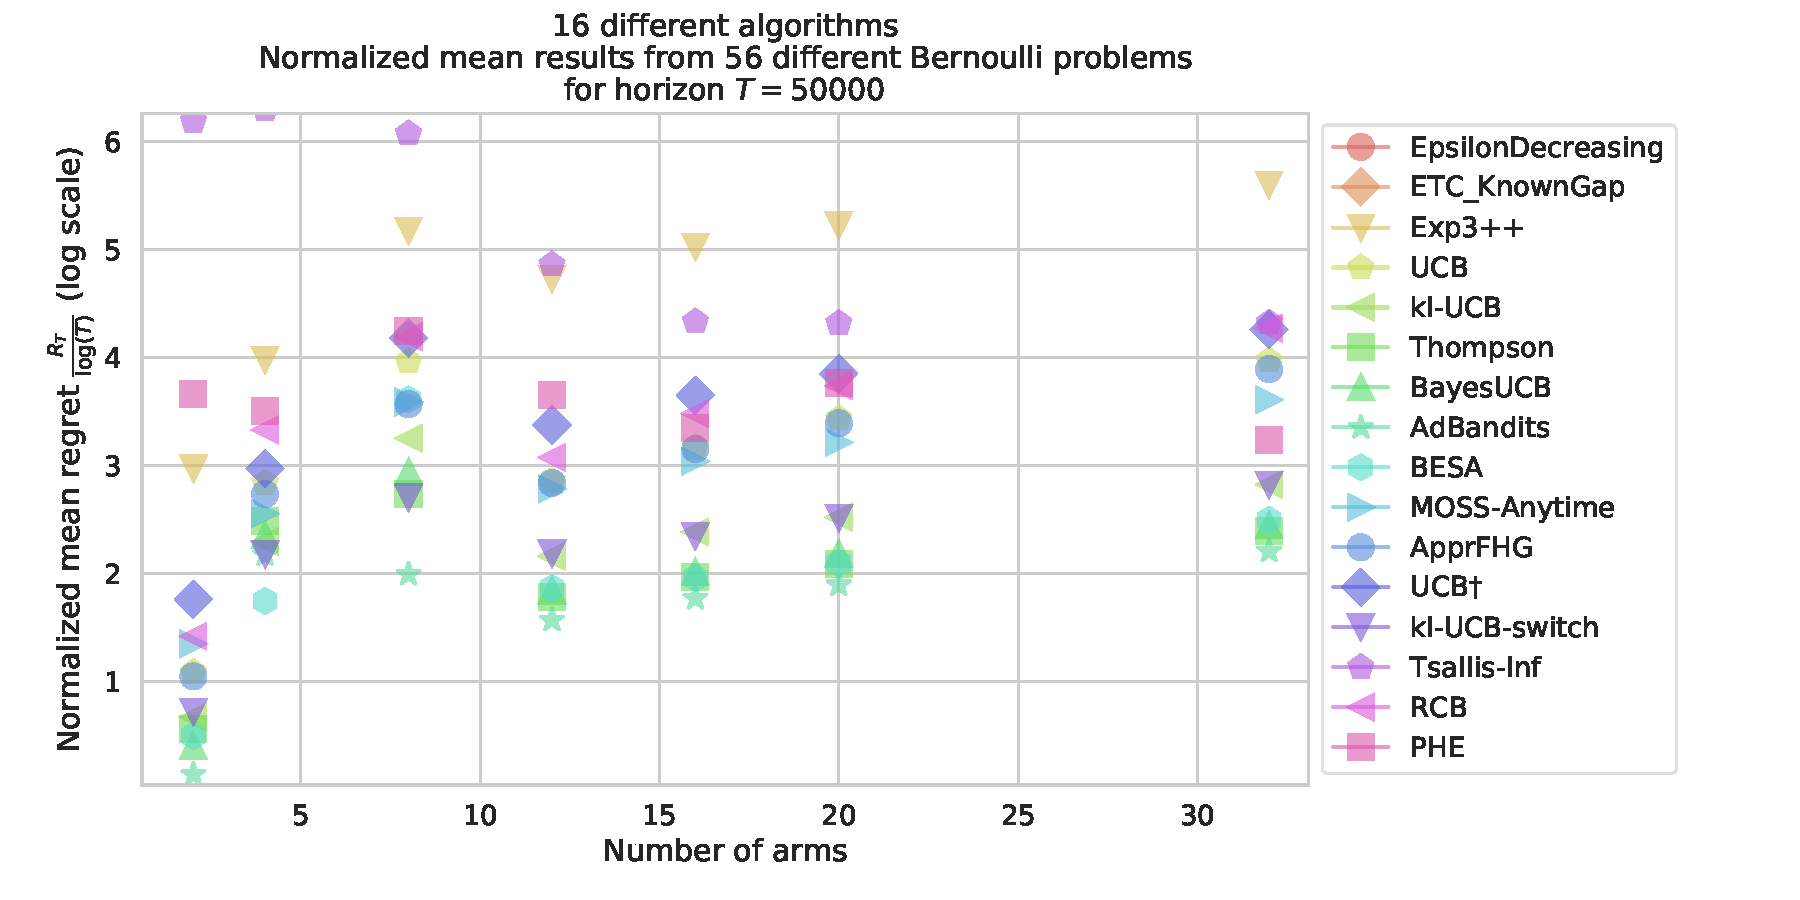
\includegraphics[width=1.10\linewidth]{16_different_algorithms__lognormregret_vs_arms__56pb__7Ks_T50000.pdf}
	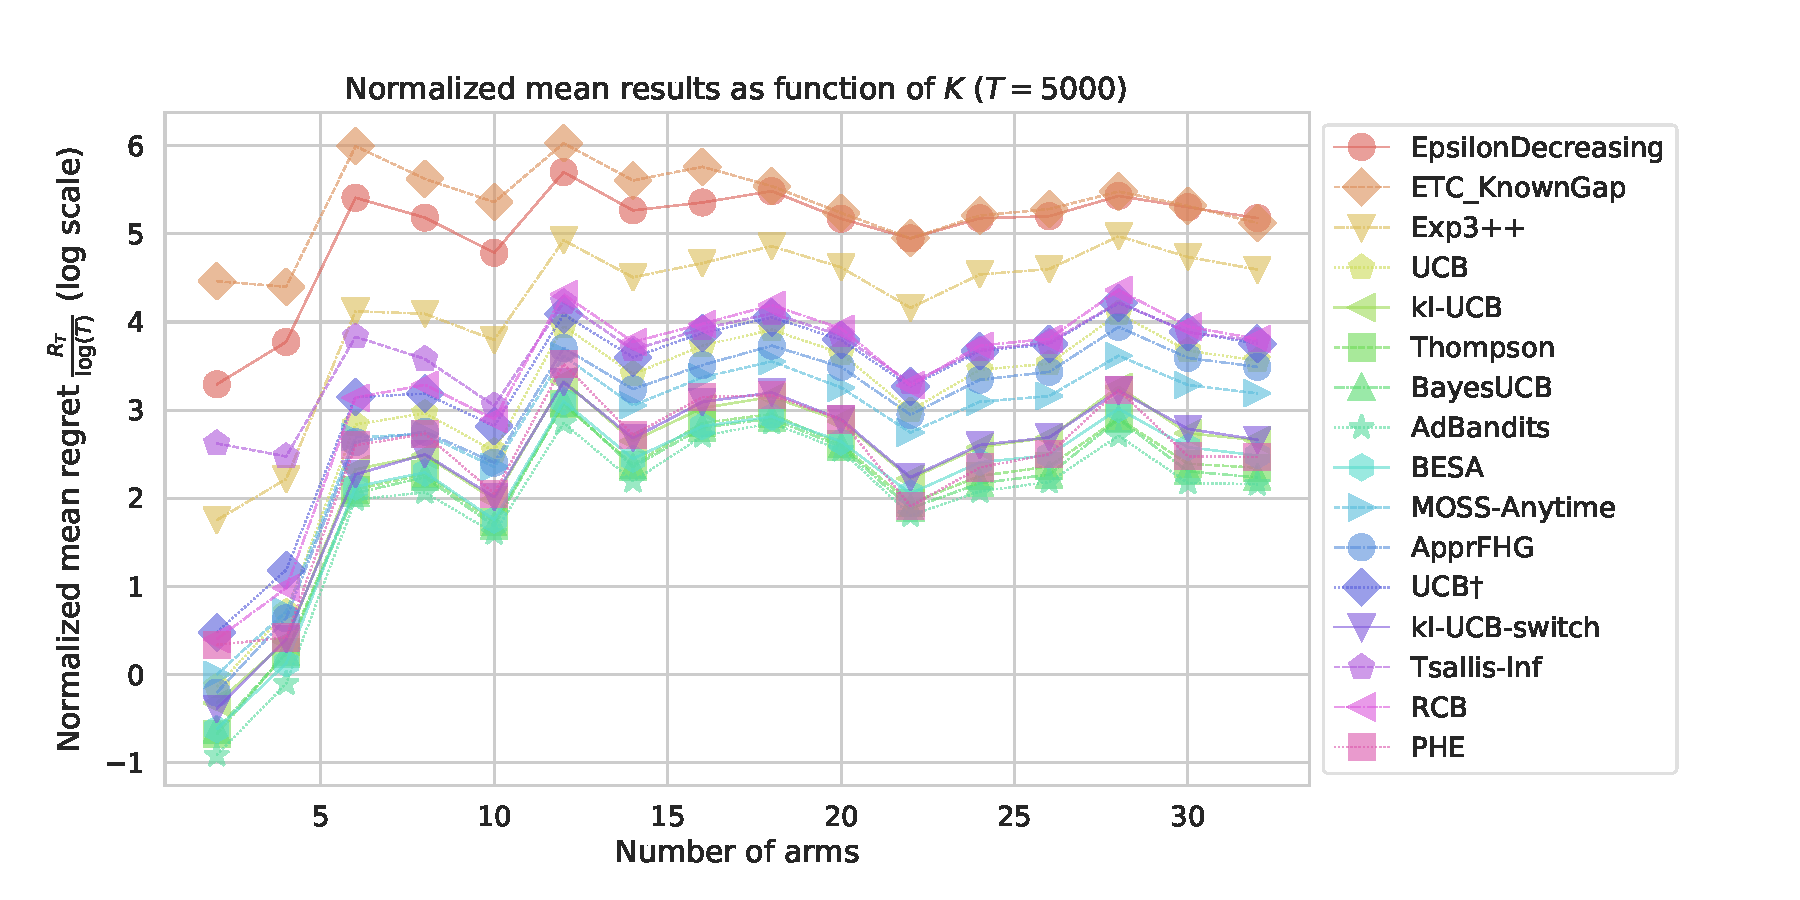
\includegraphics[width=1.10\linewidth]{16_different_algorithms__lognormregret_vs_arms__16pb__T5000.pdf}
	\caption[Regret vs different values of $K$.]{
        Regret vs different values of $K$ ($R_T / \log(T)$),
        for $T=5000$ and for $16$ algorithms.
        The $y$-axis is in log-scale.
        All algorithms appear to have a regret slowly growing with respect to $K$, as predicted by the regret bounds which are linear with respect to the number of arms.
        Bayesian algorithms appear to be the most efficient, and \klUCB{} as well as \UCB{} are also seen to be efficient.
        % \textsc{Tsallis-Inf} is the only state-of-the-art algorithm which appears to be very inefficient for problems with a small number of arms.
        Both the $\varepsilon$-greedy and Explore-then-Commit algorithms performed poorly, actually they achieve linear regret.
        % (not displayed).
	}
	\label{fig:3:16_different_algorithms__lognormregret_vs_arms__16pb__T5000}
\end{figure}

\begin{figure}[h!]  % [htbp]
	% \centering
	% 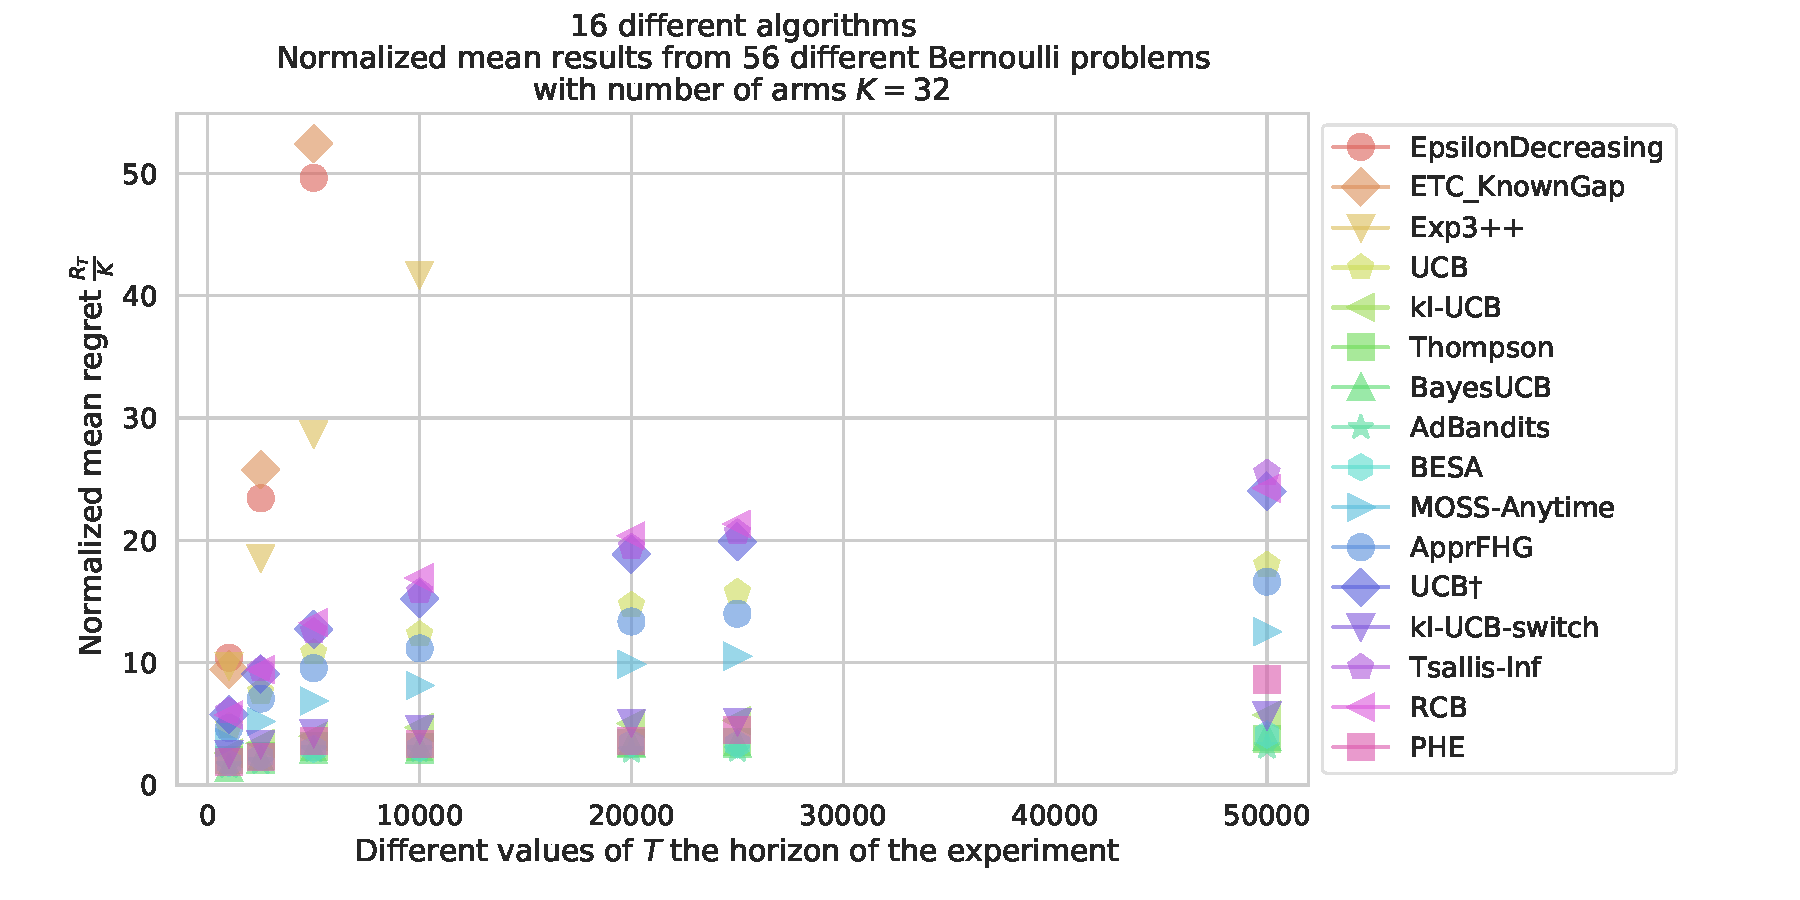
\includegraphics[width=1.10\linewidth]{16_different_algorithms__normregret_vs_horizons__56pb__K32_7Ts.pdf}
	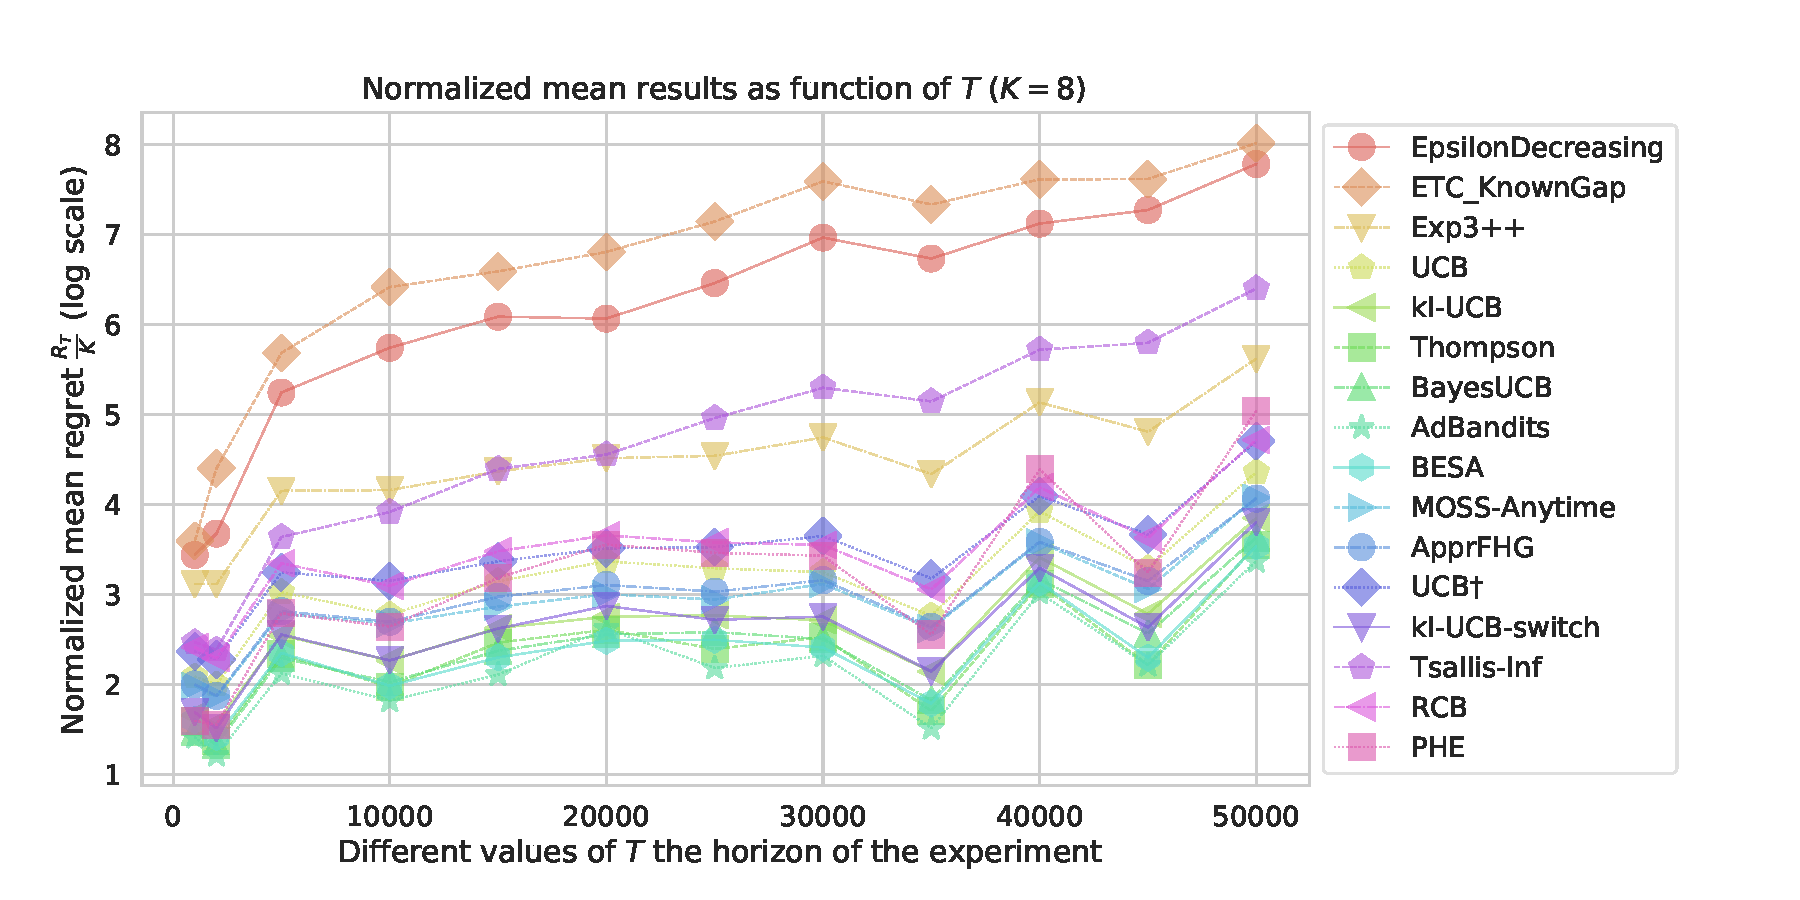
\includegraphics[width=1.10\linewidth]{16_different_algorithms__lognormregret_vs_times__16pb__K8.pdf}
	\caption[Regret vs different values of $T$.]{
        Regret vs different values of $T$ ($R_T / K$),
        for $K=32$ and for $16$ algorithms.
        All efficient algorithms appear to have a logarithmic regret with respect to the horizon, as predicted.
        The respective ranking of all the algorithms also appears to remain preserved for different values of $T$, which is also backed-up by theoretical results: if two algorithms $\cA$ and $\cA'$ has a regret close to their regret bounds, of the form $R_T \leq \cO(K \log(T))$, and the bound for $\cA$ use a smaller constant than the bound for $\cA'$, $\cA$ should obtain a smaller regret than $\cA'$ no matter the horizon.
        Bayesian algorithms appear to be the most efficient, and \klUCB{} as well as \UCB{} are also shown to be efficient.
        Finally, we also observe once more that both $\varepsilon$-greedy and Explore-then-Commit performed poorly, achieving linear regret.
	}
	\label{fig:3:16_different_algorithms__lognormregret_vs_times__16pb__K8}
\end{figure}


\paragraph{Summary of the experiments.}
%
% In the two Figures~\ref{fig:3:16_different_algorithms__lognormregret_vs_arms__16pb__T5000} and \ref{fig:3:16_different_algorithms__lognormregret_vs_times__16pb__K8}
% included in this section,
We are able to check empirically that the regret of all the efficient algorithm indeed scales as predicted by the theory, that is
linearly in the number of arms, and logarithmically in the horizon, \ie, $R_T = \bigO{K \log T}$.
%
The main take-away message is the following: in all the rest of this thesis, we focus on two algorithms depending if simplicity or efficiency is favored:
\begin{itemize}%\tightlist
    \item
    \UCB{} is used in the more applied Chapter~\ref{chapter:4}, when simplicity is favored,
    \item
    \klUCB{} is used, in the two more theoretical Chapters~\ref{chapter:5} and \ref{chapter:6}, when we analyze mathematically the performance of an algorithm that is running on top of a classical stationary MAB policy, like our two contributions, \MCTopM{} and \GLR.
\end{itemize}

% FIXME
\newpage


% ----------------------------------------------------------------------------
\section{Comparing real measurements of time and memory costs}
\label{sec:3:timeAndMemoryCosts}

In this section, we report additional experiment results from the simulations described in the previous Section~\ref{sec:3:reviewSPAlgorithms}.
Instead of studying on the efficiency of the algorithms (\ie, their regret), we report results of real measurements in terms of computational time as well as memory storage.
% %
% The goal of this section is to verify that the simplest (but most efficient) algorithms have a memory cost proportional to the number of arms but independent of the horizons, \ie, bounded by $\bigO{K}$, and a time complexity at each time step $t\in[T]$ bounded by $\bigO{K}$, independent of $t$.
%
%
While the results reported in the previous section should not depend on the implementation of the different algorithms, the results in this section concern real measurements of both time and memory consumptions of the simulation software used for these simulations.
Hence, the reported results highly depend on many factors, including how the code is written, and where and when it is run.
We take precautions to ensure the fairness of the comparison between the different algorithms, as detailed in Appendix~\ref{sub:3:precautionsTimeMemory}.


\subsection{Computational time}

In Figure~\ref{fig:3:16_different_algorithms__lognormregret_vs_logtime__28pb}, we can see that Bayesian algorithms appear to be the most efficient (\ie, in the bottom left corner), and \klUCB{} is very close to their best empirical performances.
\UCB, algorithms that were proven to perform similarly to \UCB{} (\ie, PHE and RCB), and other index policies inspired by \UCB{} (ApprFHG, $\UCB\dagger$) enjoy very similar performances: a larger regret than Bayesian algorithms and \klUCB, but a shorter running time.
%
This observation highlights an interesting trade-off between having a small regret, and being fast and computationally efficient.
%
We also observe that BESA has a low regret but is much slower than all the other algorithms, because its complexity is exponentially growing wrt $K$ the number of arms.

Moreover, in the two Figures~\ref{fig:3:16_different_algorithms__lognormtime_vs_arms__16pb__T5000} and
\ref{fig:3:16_different_algorithms__lognormtime_vs_times__16pb__K8},
we are able to check empirically that the computational time of all the efficient algorithm indeed scales as predicted by the theory, that is
linearly in the number of arms in the horizon, \ie, $\cT_T = \bigO{KT}$.

\begin{figure}[h!]  % [htbp]
	% \centering
	% 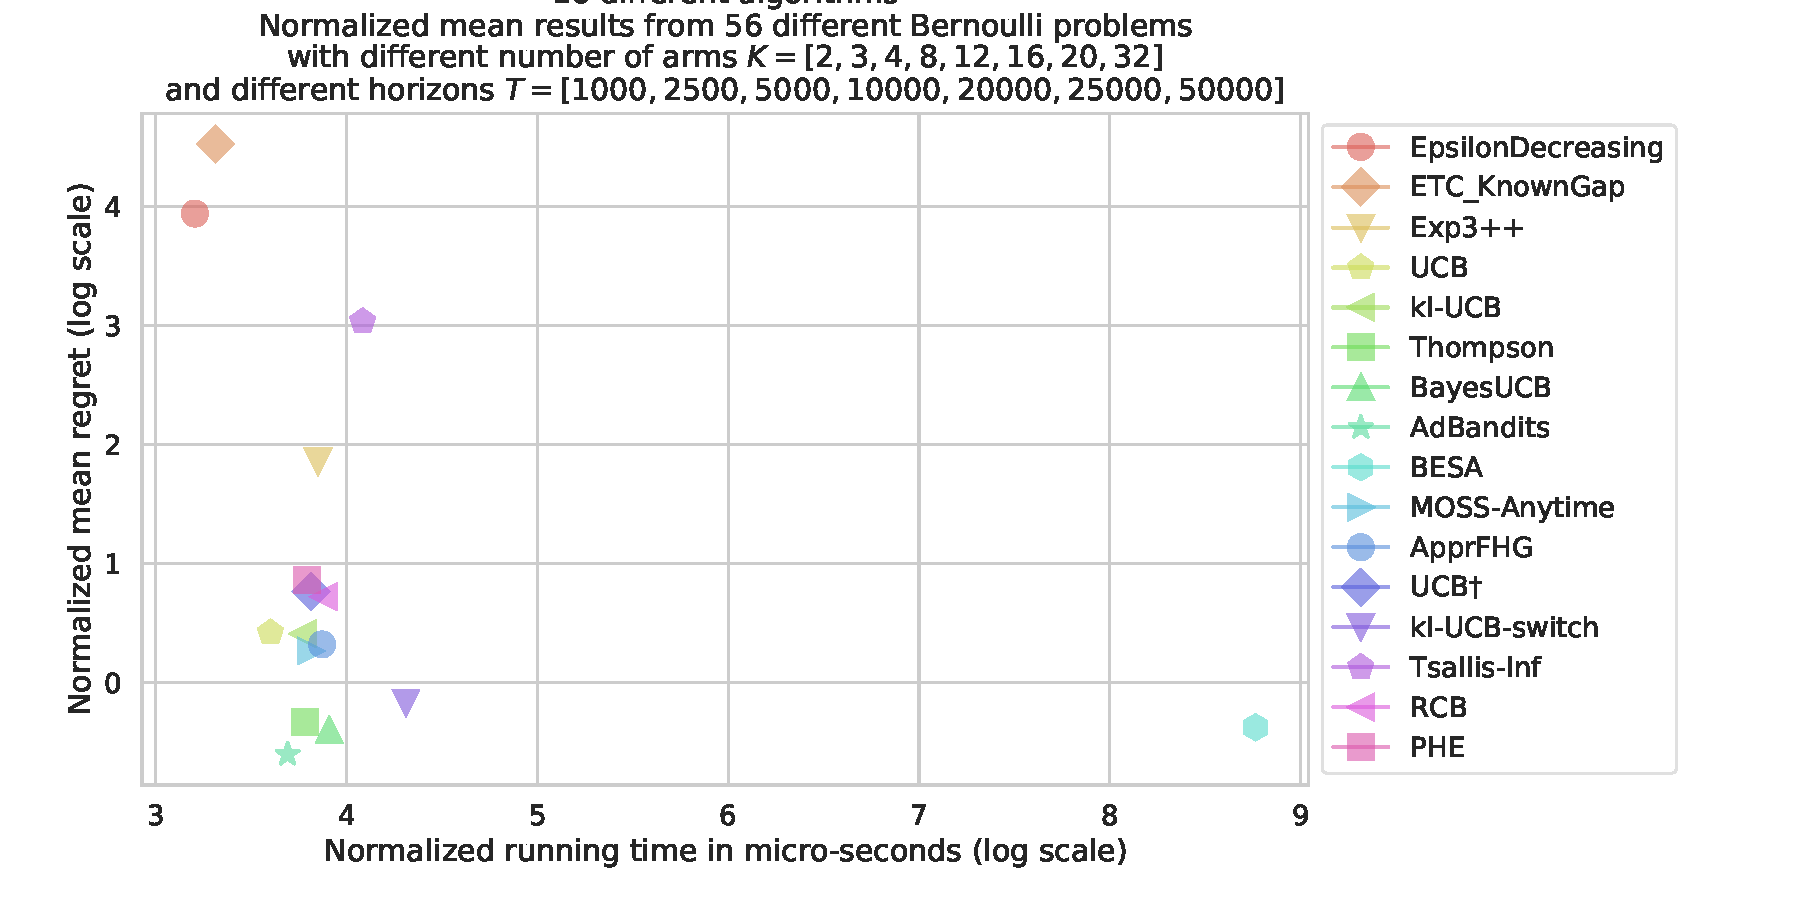
\includegraphics[width=1.10\linewidth]{16_different_algorithms__lognormregret_vs_lognormtime__56pb__7Ks_7Ts.pdf}
	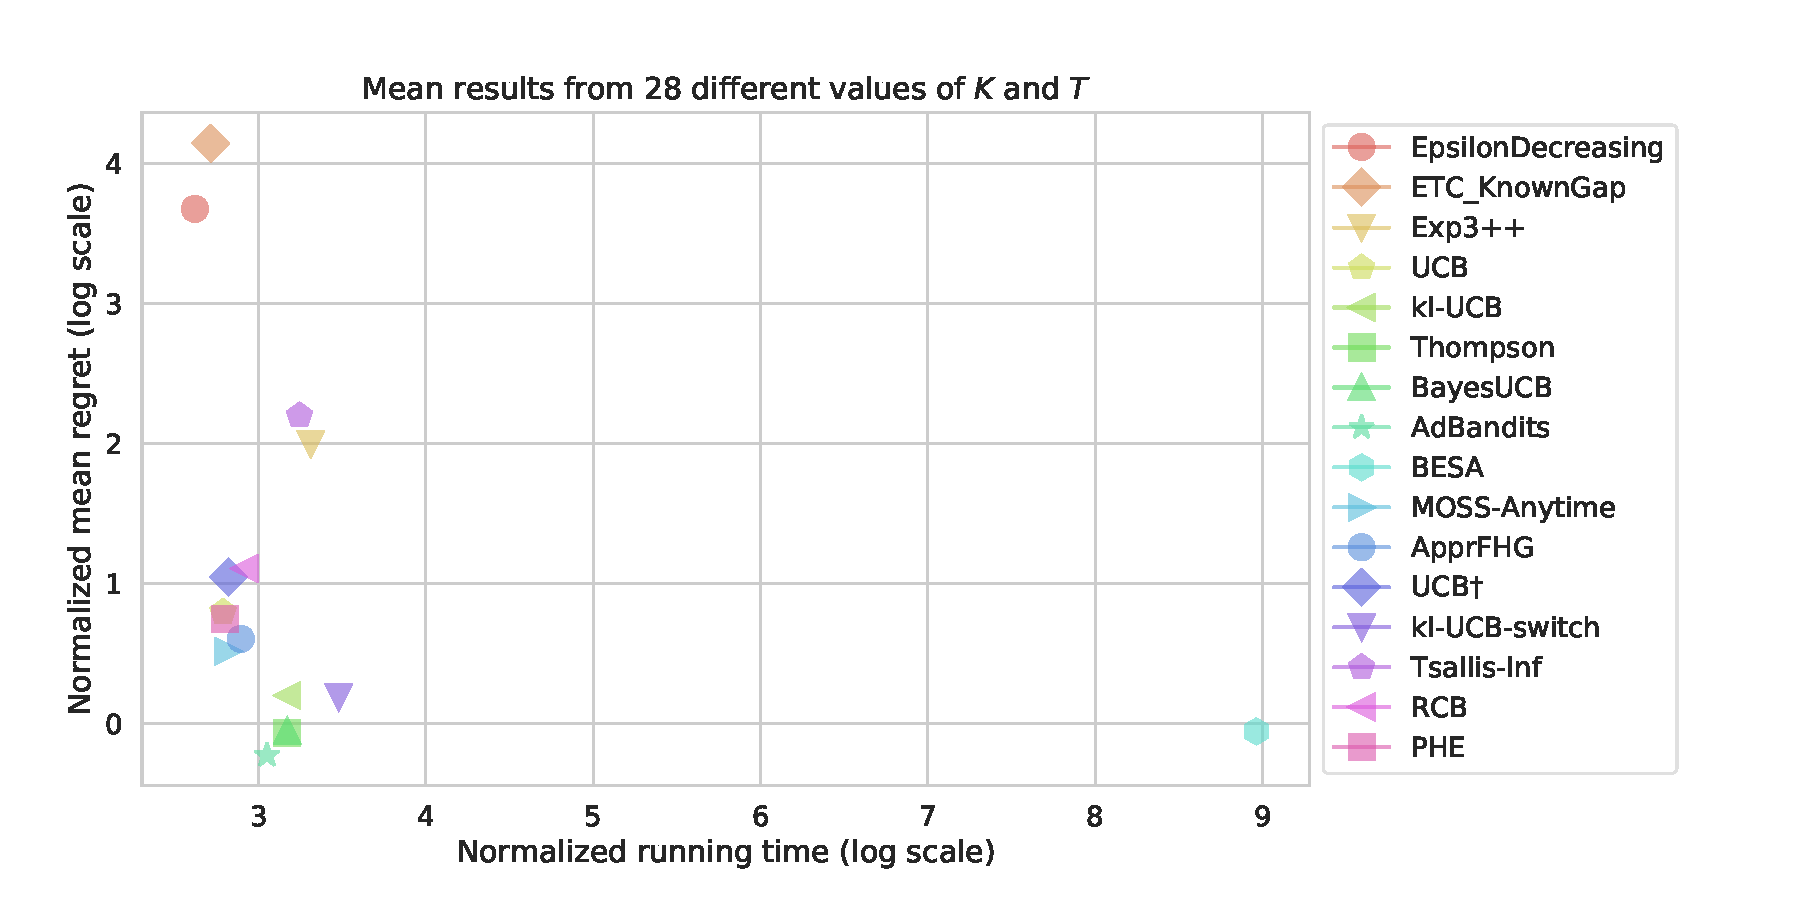
\includegraphics[width=1.10\linewidth]{16_different_algorithms__lognormregret_vs_logtime__28pb.pdf}
	\caption[Normalized mean regret vs normalized running time (in micro-seconds).]{
        Normalized mean regret vs normalized running time (in micro-seconds),
        aggregating the results from different values of $K$ and $T$, for $16$ algorithms.
        Both the $x$-axis and $y$-axis are in log-scale.
        \UCB{} and \klUCB{} are among the best algorithms, while AdBandits, Thompson sampling and Bayes-UCB slightly outperform them in terms of regret, and have similar running times.
	}
	\label{fig:3:16_different_algorithms__lognormregret_vs_logtime__28pb}
\end{figure}


\begin{figure}[h!]  % [htbp]
	% \centering
	% 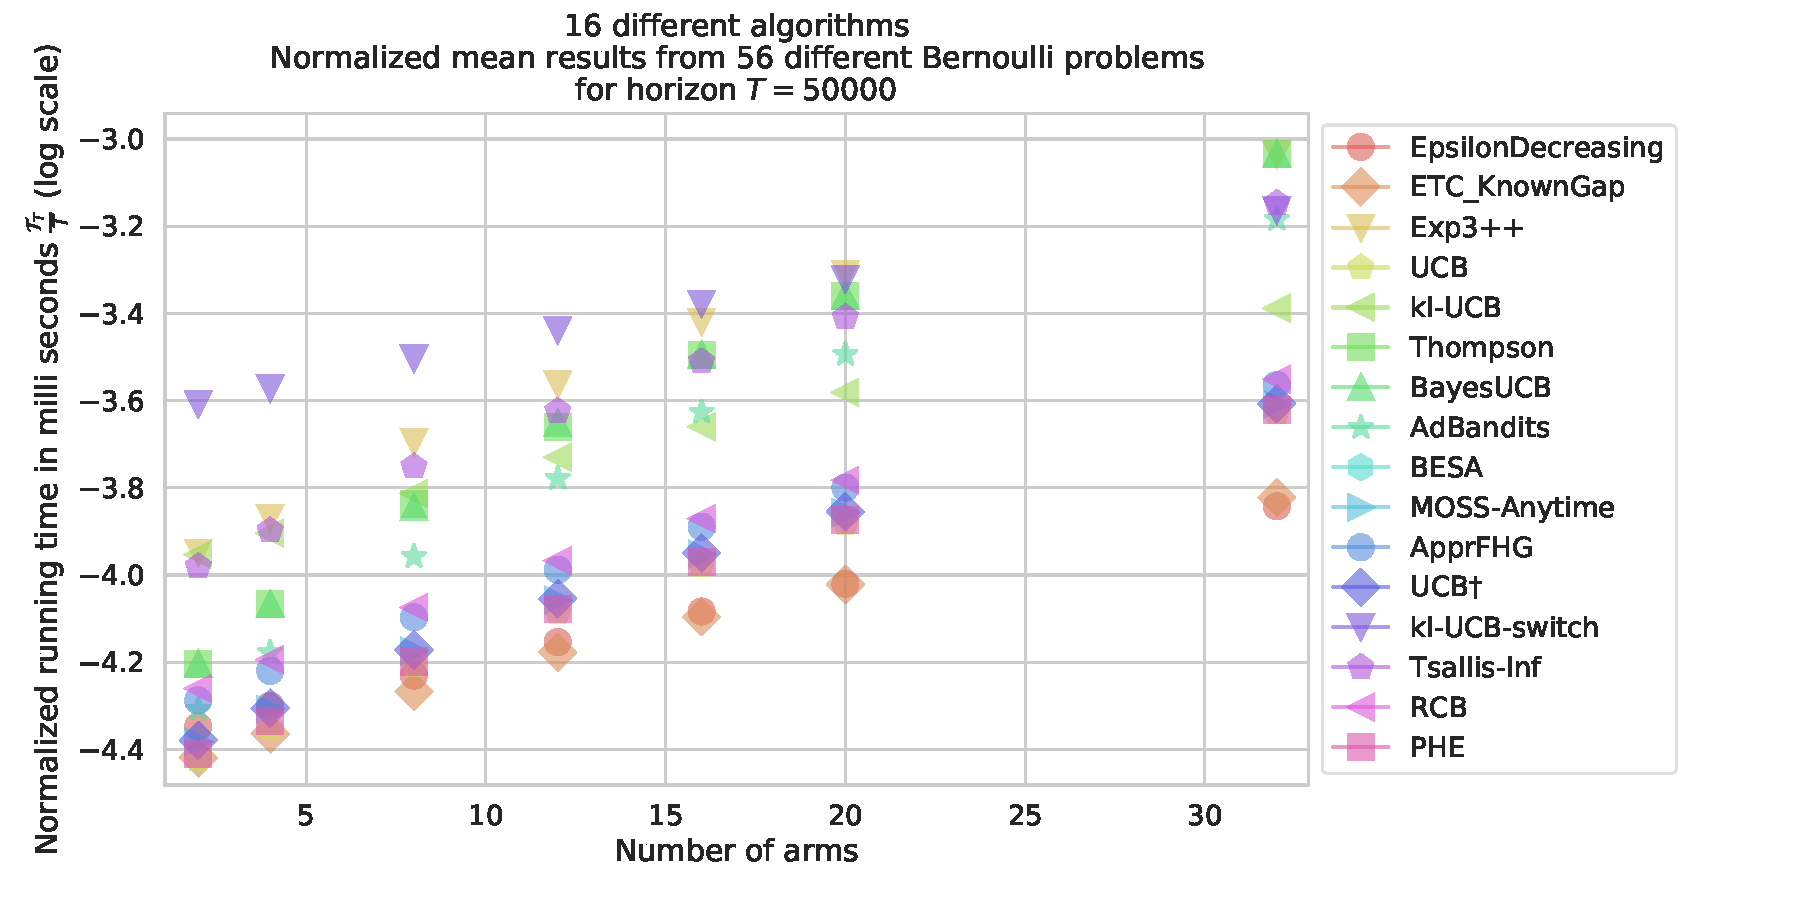
\includegraphics[width=1.10\linewidth]{16_different_algorithms__lognormtime_vs_arms__56pb__7Ks_T50000.pdf}
	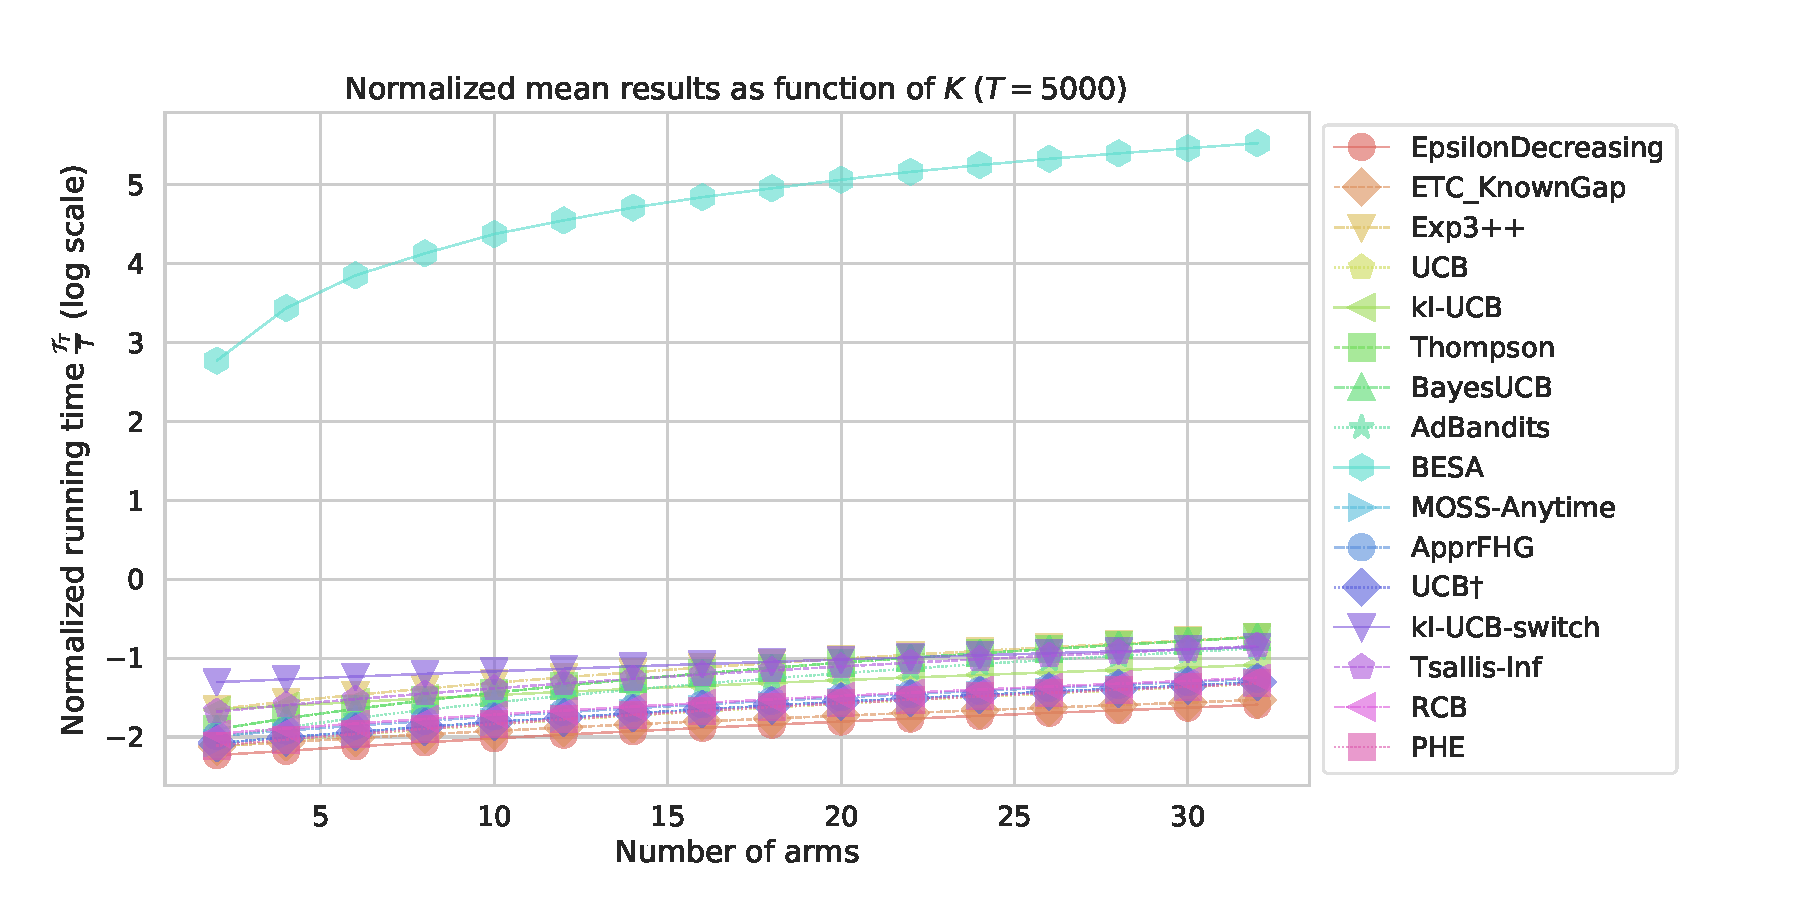
\includegraphics[width=1.10\linewidth]{16_different_algorithms__lognormtime_vs_arms__16pb__T5000.pdf}
	\caption[Normalized running time vs different values of $K$.]{
        Normalized running time vs different values of $K$ ($\cT_T / T$),
        for $T=5000$ and for $16$ algorithms.
        $y$-axis is in log-scale.
        All algorithms except BESA has a linear normalized running time, meaning that for $K$ arms they use a computation time proportional to $K$, as predicted: $\cT_T = \bigO{KT}$.
	}
	\label{fig:3:16_different_algorithms__lognormtime_vs_arms__16pb__T5000}
\end{figure}

\begin{figure}[h!]  % [htbp]
	% \centering
	% 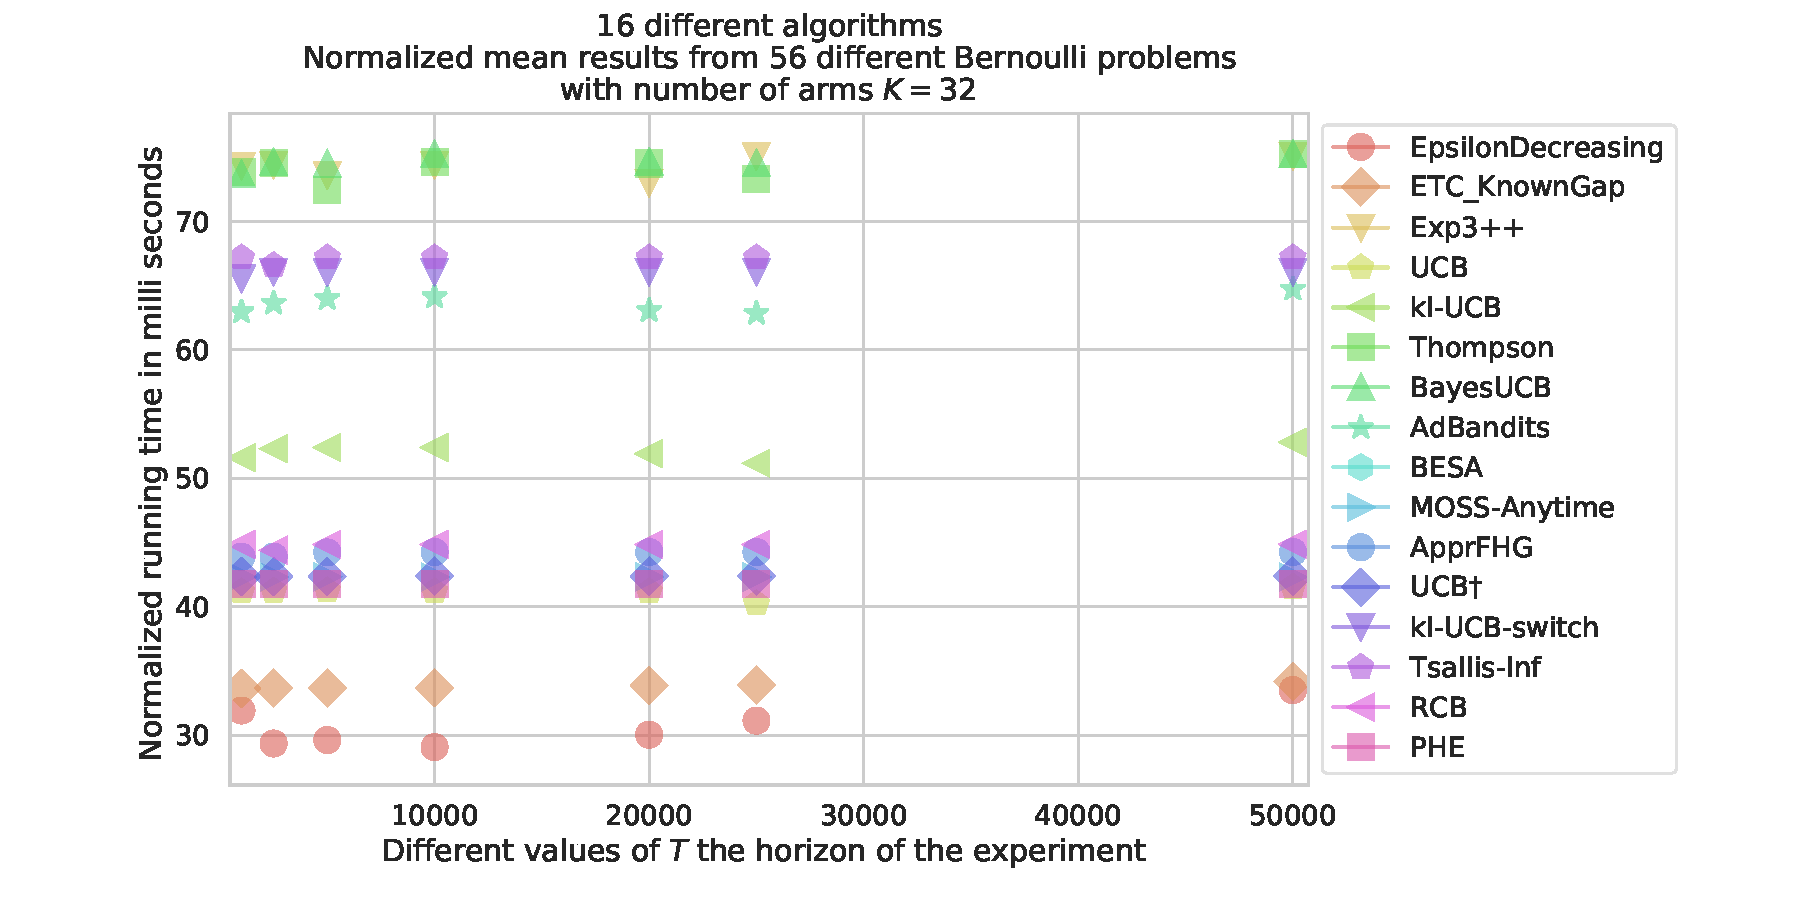
\includegraphics[width=1.10\linewidth]{16_different_algorithms__normtime_vs_horizons__56pb__K32_7Ts.pdf}
	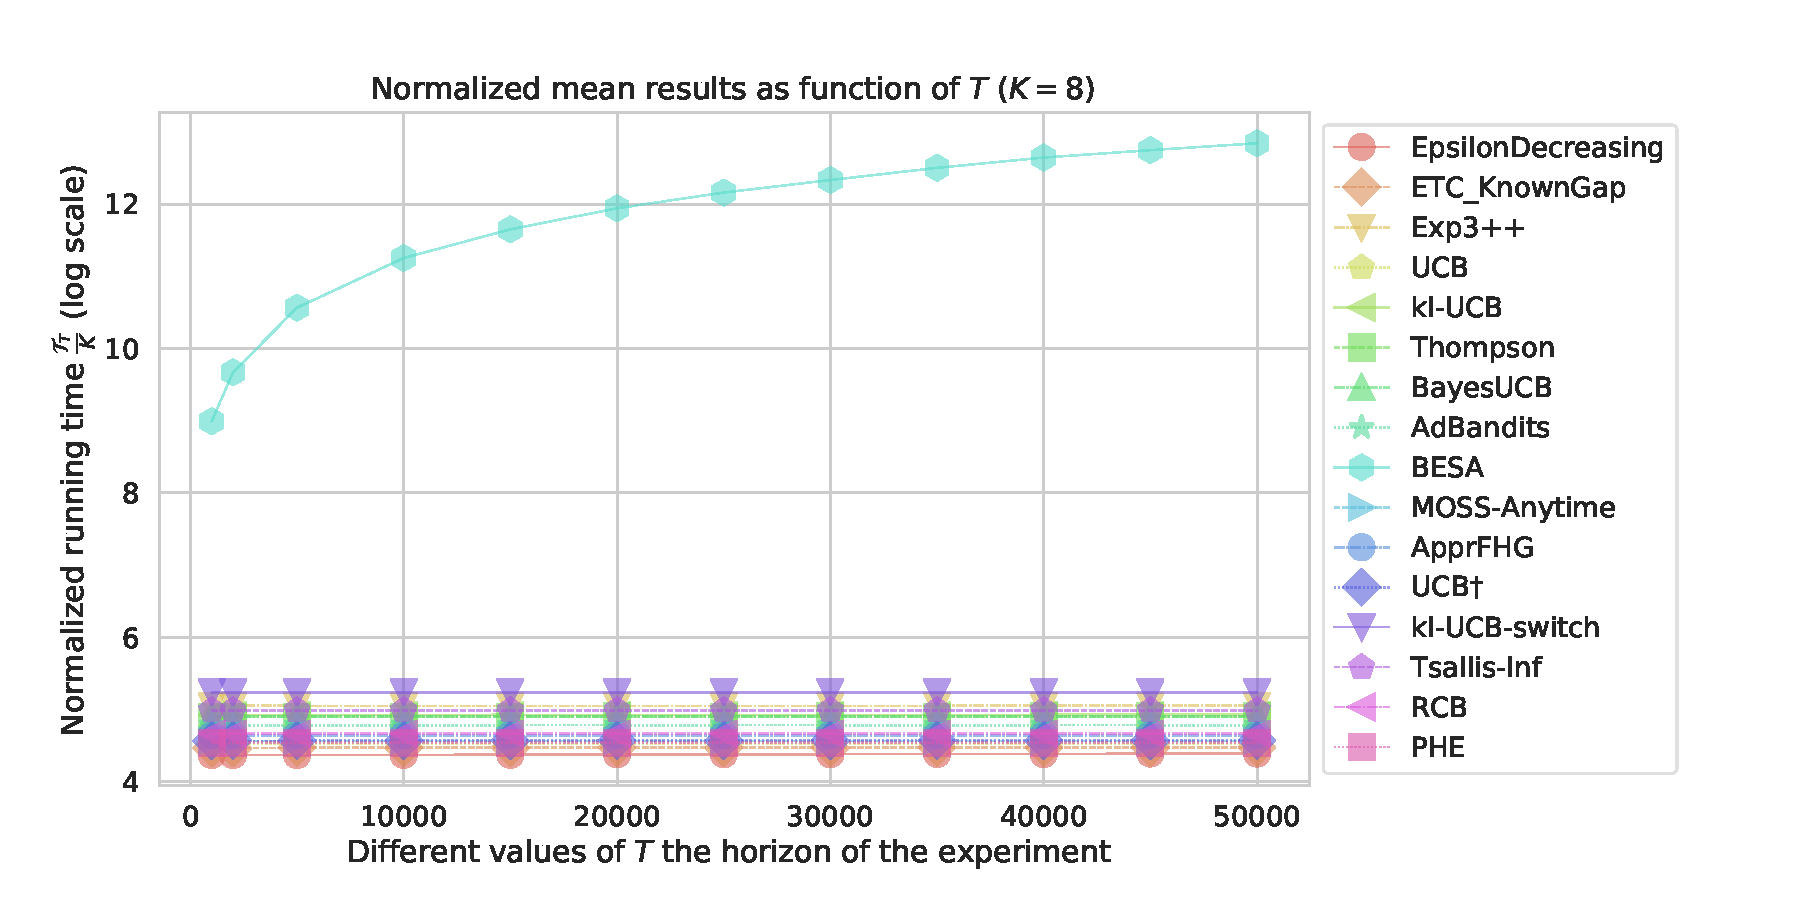
\includegraphics[width=1.10\linewidth]{16_different_algorithms__lognormtime_vs_times__16pb__K8.pdf}
	\caption[Normalized running time vs different values of $T$.]{
        Normalized running time vs different values of $T$ ($\cT_T / T$),
        for $K=32$ and for $16$ algorithms.
        $y$-axis is in log-scale.
        All algorithms except BESA has a constant normalized running time, meaning that for $T$ rounds they use a computation time proportional to $T$, as predicted: $\cT_T = \bigO{KT}$.
	}
	\label{fig:3:16_different_algorithms__lognormtime_vs_times__16pb__K8}
\end{figure}


\subsection{Memory cost}

Like for the computational cost discussed above,
in Figure~\ref{fig:3:16_different_algorithms__lognormregret_vs_logmemory__28pb}, we can see that Bayesian algorithms like Thompson sampling again appear to be the most efficient (\ie, in the bottom left corner), and \klUCB{} is close to their best empirical performances.
\UCB{} and other index policies inspired by \UCB{} (ApprFHG, $\UCB\dagger$) enjoy very similar performances: a larger regret than Bayesian algorithms and \klUCB, but a similar memory cost.
%
This time, there is no clear trade-off between optimality in terms of regret and memory cost, and based on simply this Figure~\ref{fig:3:16_different_algorithms__lognormregret_vs_logmemory__28pb}, one could advise to use Thompson sampling rather than \klUCB.

Moreover, in the two Figures~\ref{fig:3:16_different_algorithms__lognormmemory_vs_arms__16pb__T5000} and
\ref{fig:3:16_different_algorithms__lognormmemory_vs_times__16pb__K8},
we are able to check empirically that the memory cost of all the efficient algorithm indeed scales as predicted by the theory, that is
linearly in the number of arms but independently of the horizon, \ie, $\cM_T = \bigO{K}$.

\begin{figure}[h!]  % [htbp]
	% \centering
	% 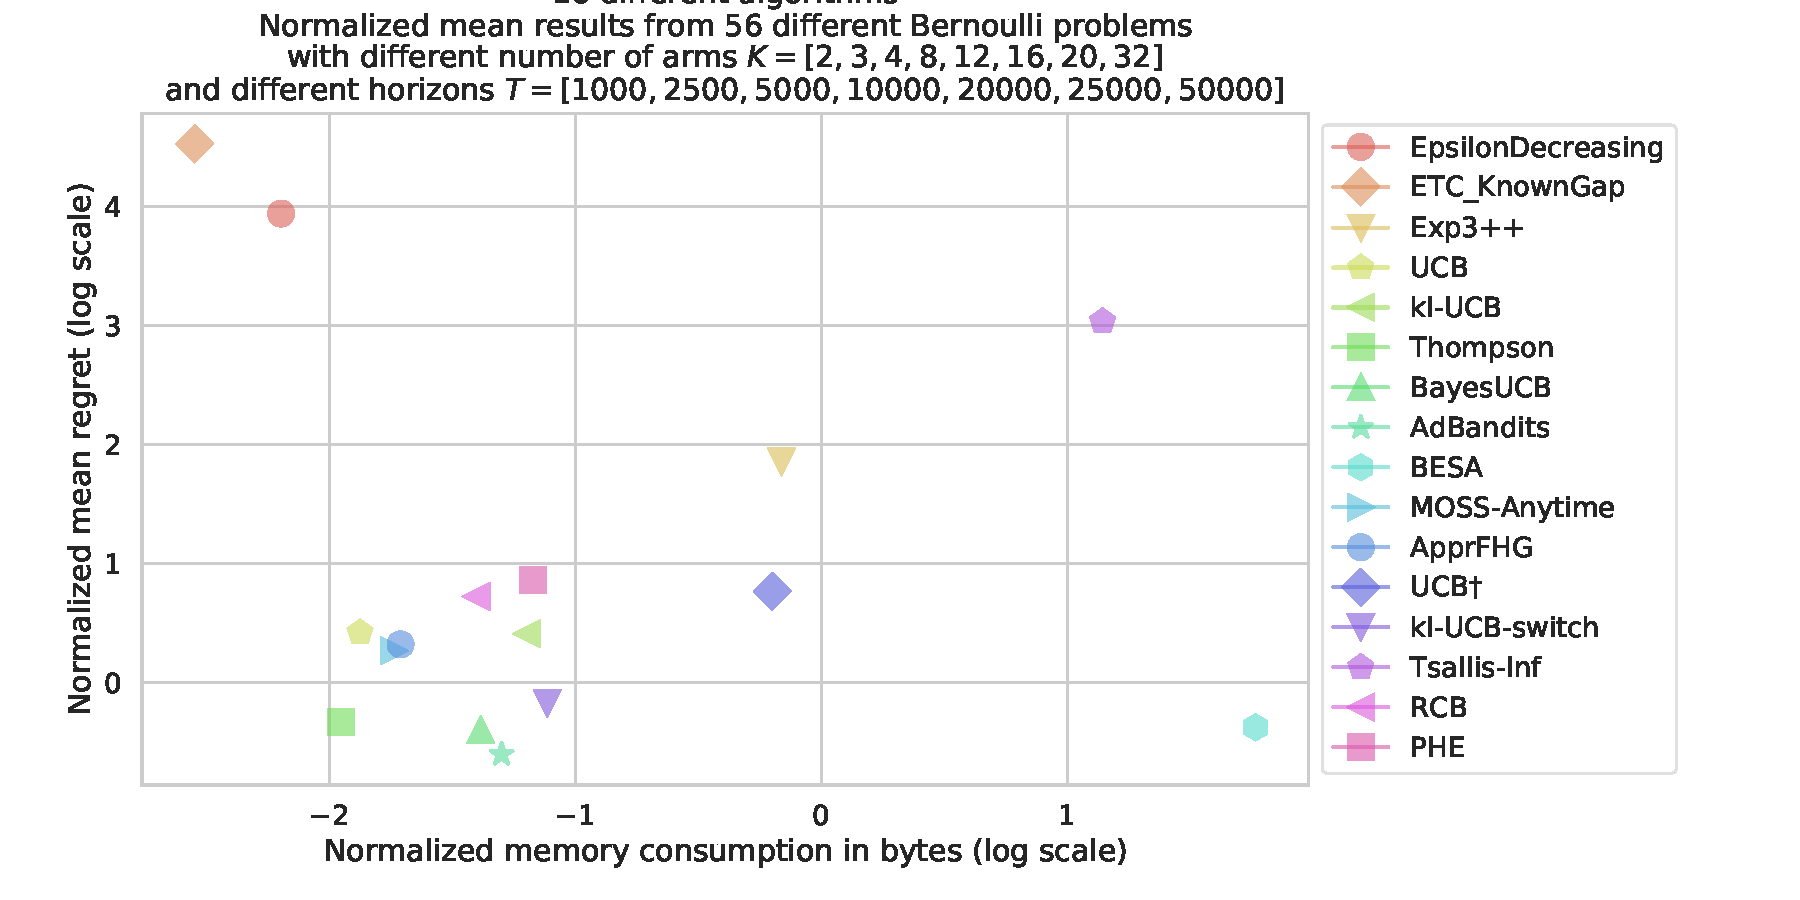
\includegraphics[width=1.10\linewidth]{16_different_algorithms__lognormregret_vs_lognormmemory__56pb__7Ks_7Ts.pdf}
	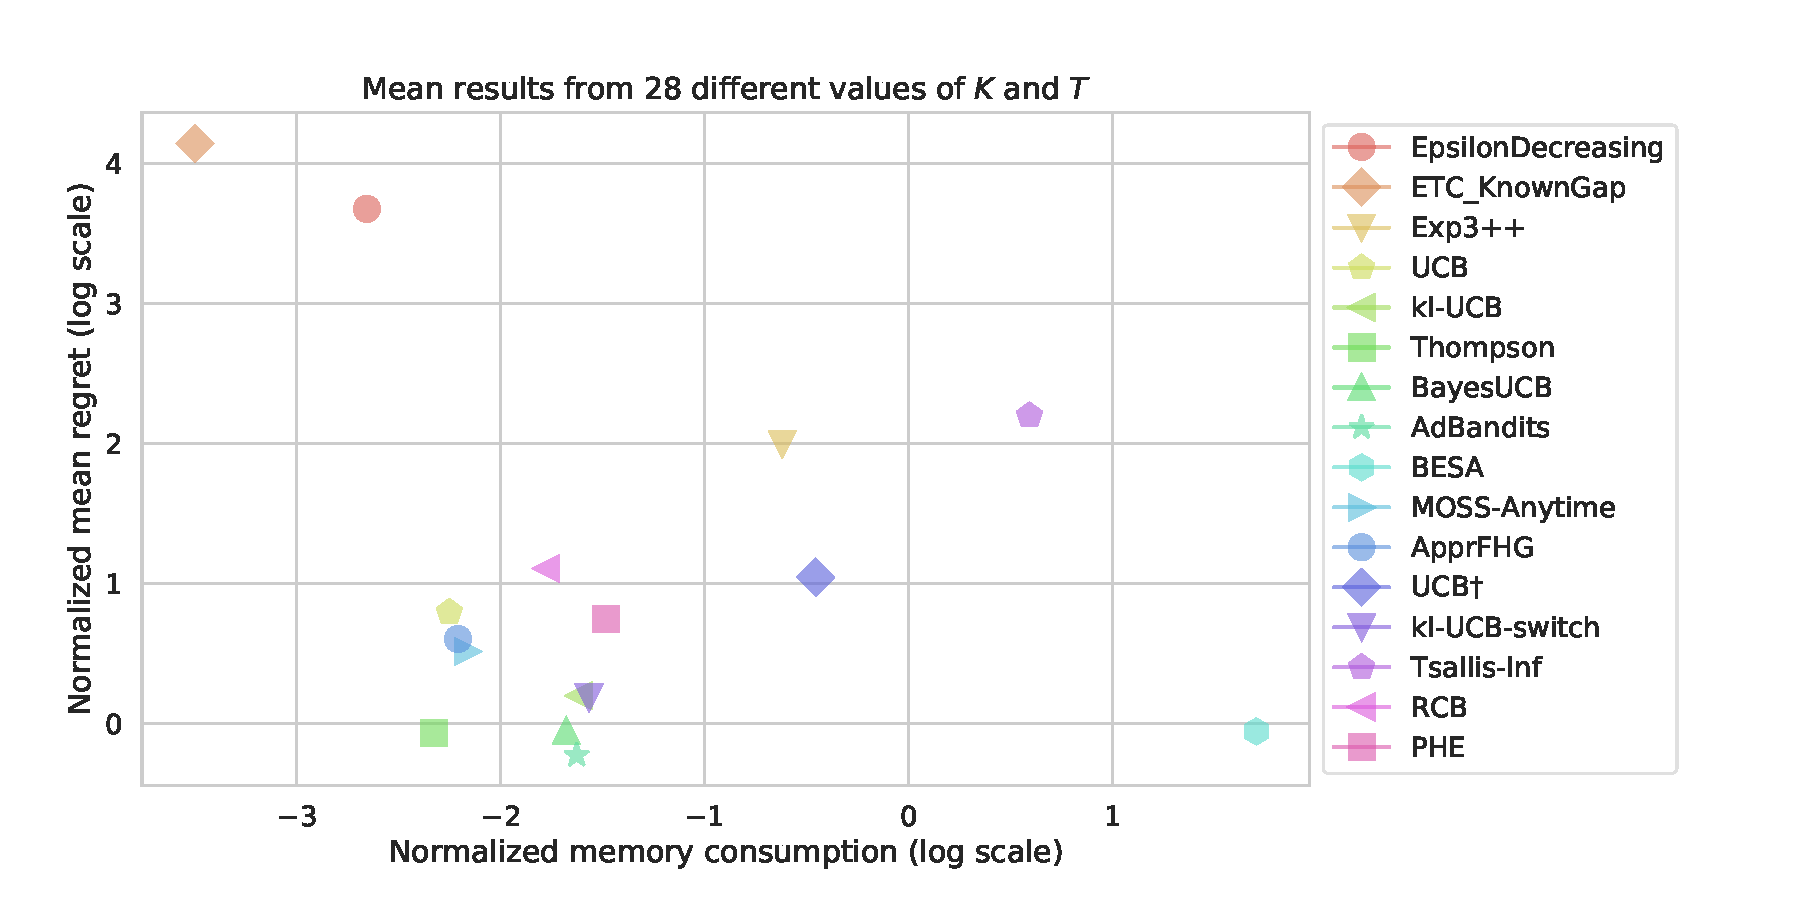
\includegraphics[width=1.10\linewidth]{16_different_algorithms__lognormregret_vs_logmemory__28pb.pdf}
	\caption[Normalized mean regret vs normalized memory costs (in bytes).]{
        Normalized mean regret vs normalized memory costs (in bytes),
        aggregating the results from different values of $K$ and $T$, for $16$ algorithms.
        Both the $x$-axis and $y$-axis are in log-scale.
        Thompson sampling appears as the best algorithm in this visualization, while \UCB{} has the advantage of being memory efficient, and \klUCB{} obtains similar performances.
	}
	\label{fig:3:16_different_algorithms__lognormregret_vs_logmemory__28pb}
\end{figure}


\begin{figure}[h!]  % [htbp]
	% \centering
	% 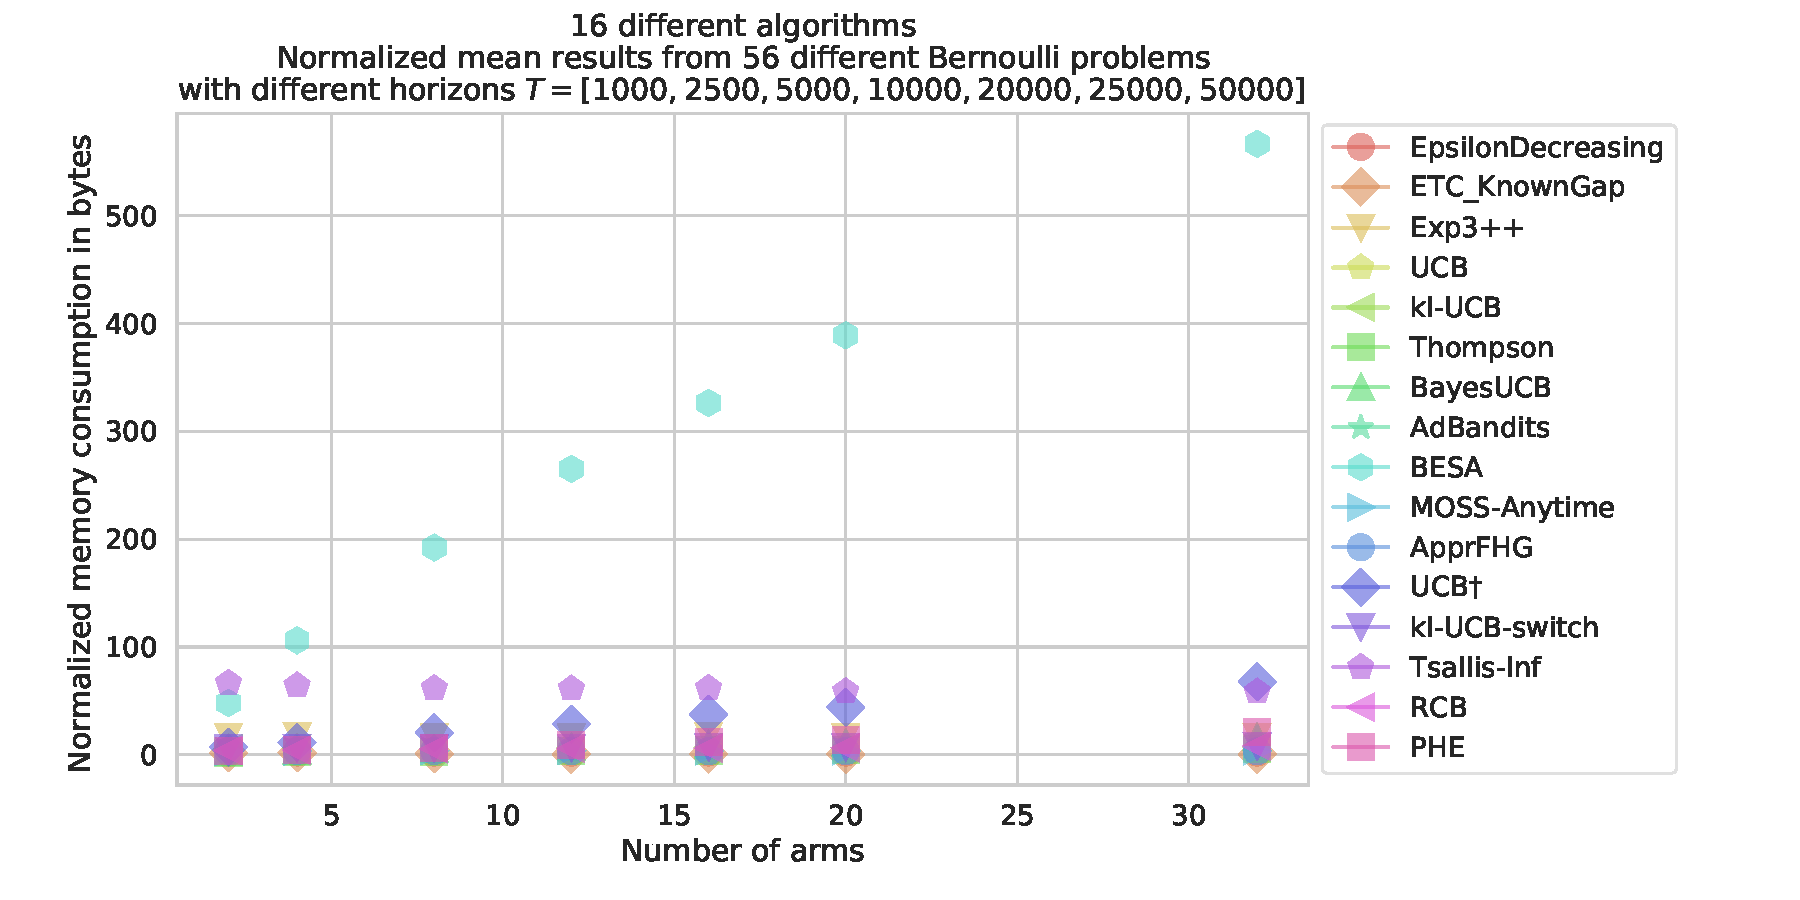
\includegraphics[width=1.10\linewidth]{16_different_algorithms__normmemory_vs_arms__56pb__7Ks_T50000.pdf}
	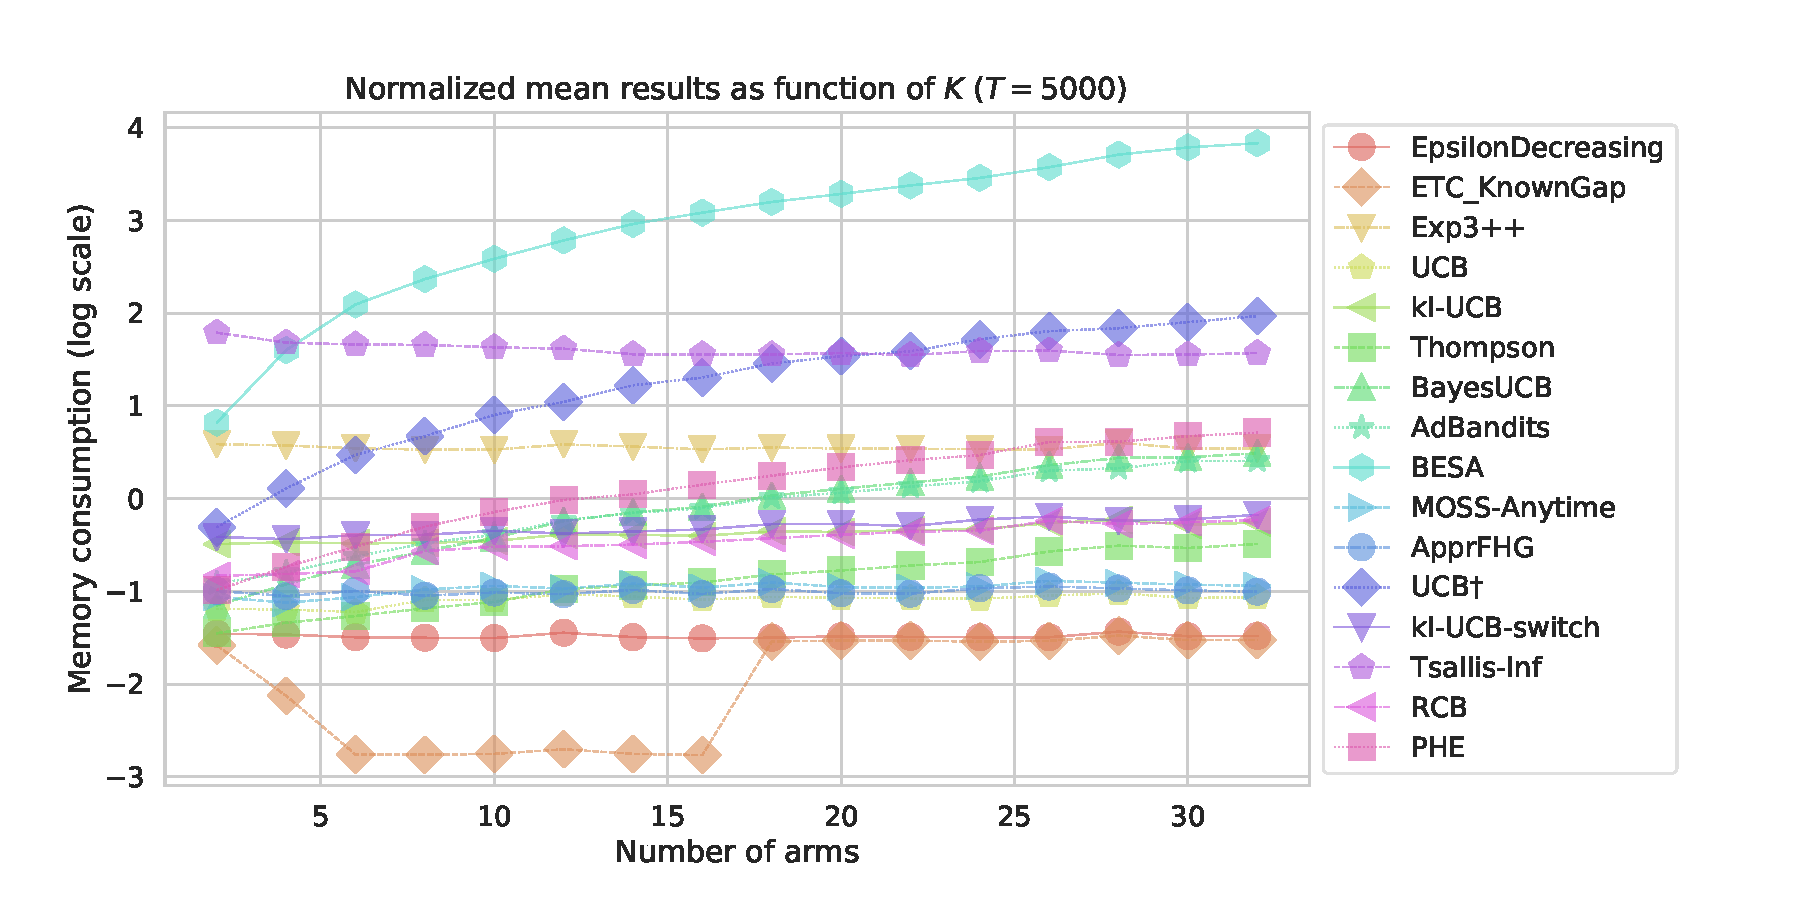
\includegraphics[width=1.10\linewidth]{16_different_algorithms__lognormmemory_vs_arms__16pb__T5000.pdf}
	\caption[Normalized memory cost vs different values of $K$.]{
        Normalized memory cost vs different values of $K$ ($\cM_T / K$),
        for $T=5000$ and for $16$ algorithms.
        $y$-axis is in log-scale.
        All algorithms (except BESA) has an almost constant memory cost, meaning that for $K$ arms they use a storage proportional to $K$, as predicted: $\cM_T = \bigO{K}$.
	}
	\label{fig:3:16_different_algorithms__lognormmemory_vs_arms__16pb__T5000}
\end{figure}

\begin{figure}[h!]  % [htbp]
	% \centering
	% 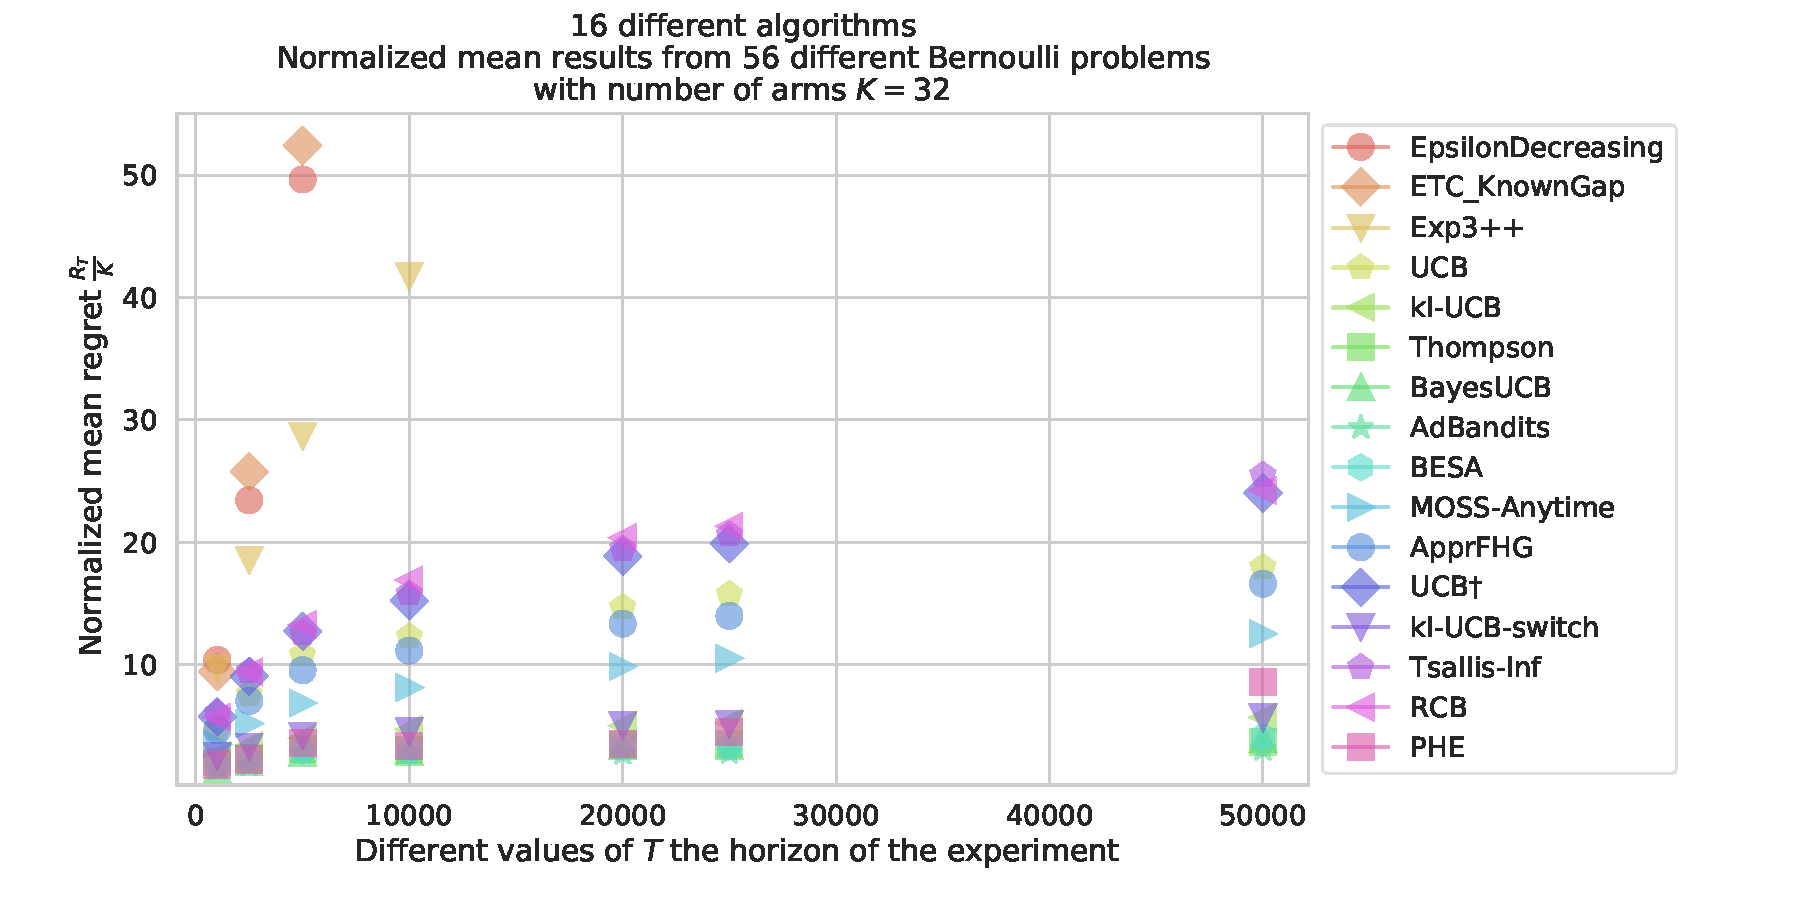
\includegraphics[width=1.10\linewidth]{16_different_algorithms__normmemory_vs_horizons__56pb__K32_7Ts.pdf}
	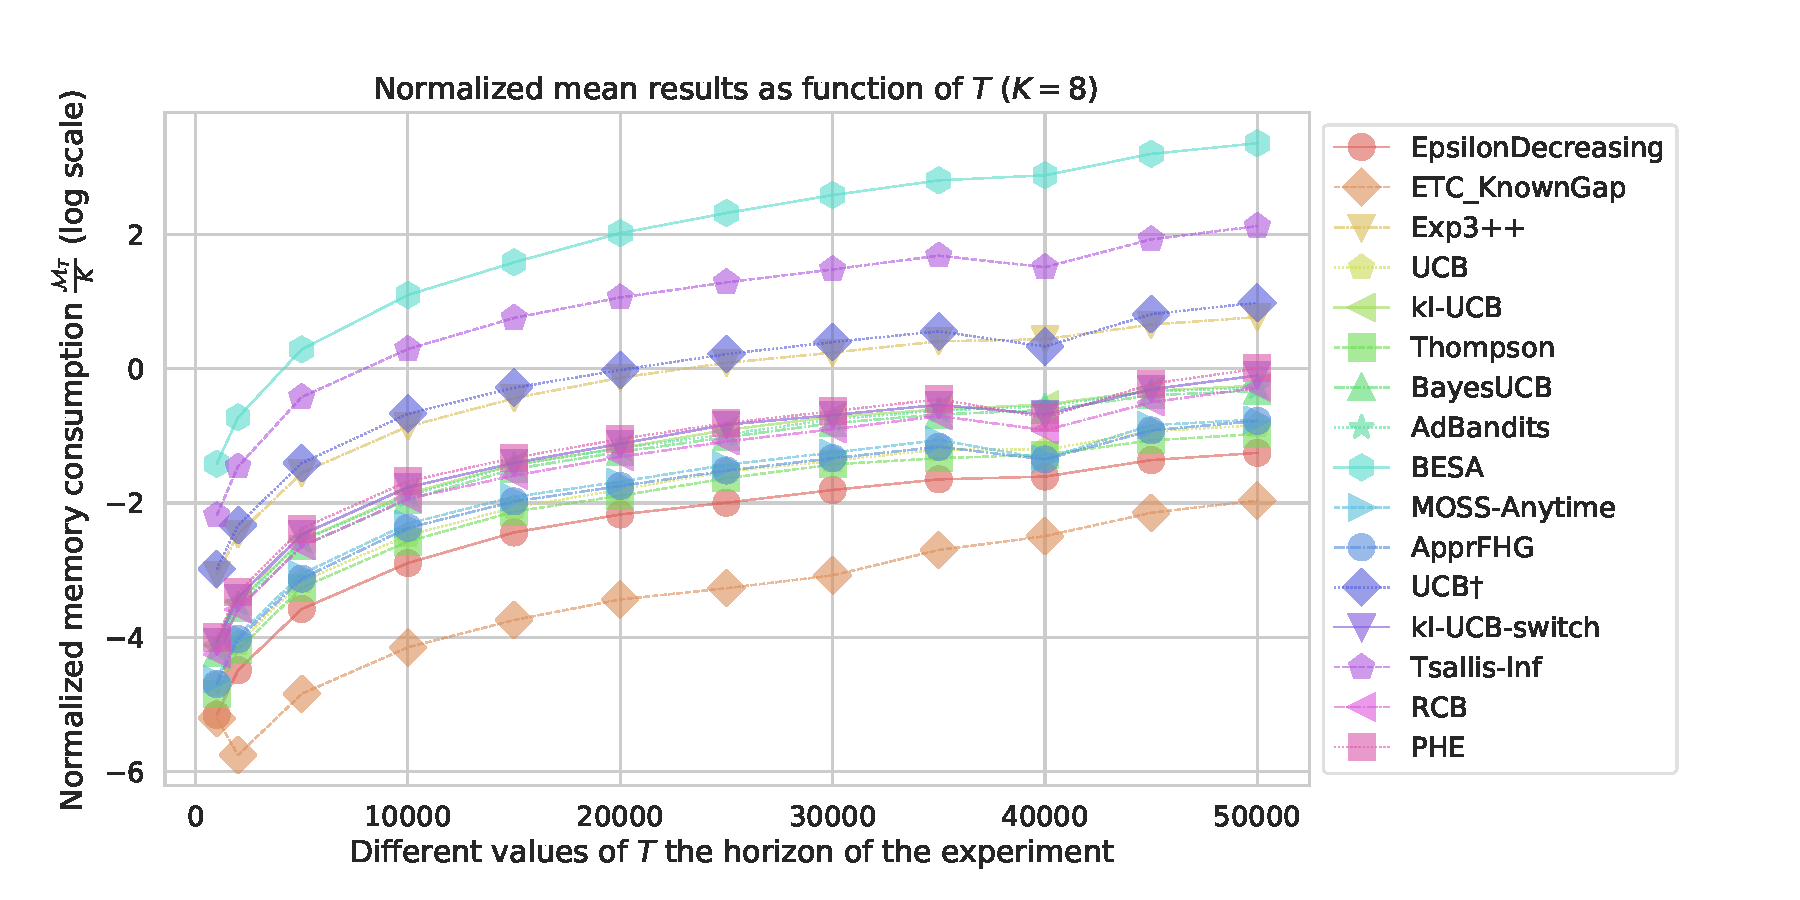
\includegraphics[width=1.10\linewidth]{16_different_algorithms__lognormmemory_vs_times__16pb__K8.pdf}
	\caption[Normalized memory cost vs different values of $T$.]{
        Normalized memory cost vs different values of $T$ ($\cM_T / K$),
        for $K=32$ and for $16$ algorithms.
        $y$-axis is in log-scale.
        All algorithms have a growing normalized memory cost, meaning that for $T$ rounds they use a computation time almost independent of $T$, as predicted: $\cM_T = \bigO{K}$.
        % All algorithms (except BESA) have a very slowly growing normalized memory cost, meaning that for $T$ rounds they use a computation time almost independent of $T$, as predicted: $\cM_T = \bigO{K}$.
        % There is a clear separation between three groups.
        % First, BESA is very costly in terms of memory, and $\UCB\dagger$ and \textsc{Tsallis-Inf} are also more costly than others, and both experiences a linear growth of their memory cost.
        % Then, we see PHE, $\mathrm{Exp}3^{++}$, Bayes-UCB and AdBandits having a small but linear growth of memory cost, and it can be explained for each of them (\eg, for Bayes-UCB, computing a quantile at time $t$ becomes more and more costly as $t$ grows, and thus as $T$ grows,  ).
        % Finally, the other algorithms (including \UCB, \klUCB{} and Thompson sampling) have a very small footprint and their memory cost do not grow much when $T$ increases.
	}
	\label{fig:3:16_different_algorithms__lognormmemory_vs_times__16pb__K8}
\end{figure}



% FIXME
% \newpage

\paragraph{Conclusion.}
%
% The main take-away message is the following:
The simplest (but most efficient) algorithms have
a time complexity at each time step $t\in[T]$ bounded by $\bigO{K}$, independently of $t$, and thus have a total time complexity bounded by $\cT_T = \bigO{KT}$,
as well as a memory cost proportional to the number of arms but independent of the horizons, \ie, bounded by $\cM_T = \bigO{K}$.

We also shown a trade-off between optimality in terms of regret, and efficiency in terms of time complexity or memory cost.
Our position regarding this trade-off is motivated by Occam's razor principle.
On the first hand, if the algorithm should be implemented on a cognitive radio device that has limited hardware capacity (for instance),
one can reasonably aim at the simplest yet order-optimal algorithms, and we advise to use \UCB{} and algorithms running on top of this simple index policy, as we do in Chapter~\ref{chapter:4}.
On the other hand, if one is more interested in the mathematical developments and wants to prove the tightest possible regret upper bounds, aiming at more efficient but more complex algorithms is interesting, and we chose the \klUCB{} algorithm in Chapters~\ref{chapter:5} and \ref{chapter:6}.


% I want to show the real numerical costs in terms of computation time and storage requirement of the various algorithms for single-player bandits.

% Maybe I can pick one simple problem family (\eg, evenly spaced in $[\varepsilon,1-\varepsilon]$), and run experiments for $T=1000,5000,10000$ etc, and $K=2,3,5,9,20,30,50,100,1000$ and show the evolution of time/memory as a function of $T$ and $K$.

% The goal is to highlight that the simplest (but most efficient) algorithms have a memory cost bounded by $\bigO{K}$ and a time complexity at each time step $t\in[T]$ bounded by $\bigO{K}$, independent of $t$.


% % ----------------------------------------------------------------------------
% \section{An example of another model: rested or restless Markov models}
% \label{sec:3:markovModels}

% %  - FIXME maybe not included?

% Maybe if I have space at the end of this chapter, I can show another part of the library, maybe introduce the rested/restless Markov models (with maybe just one example) and show simulations in this model?

% SMPyBandits also implemented sparse MAB models (with $s<K$ arms with a mean $\mu_i>0$ and $K-s$ arms with a mean $\mu_i \leq 0$), I could also present this model, the various algorithms designed to tackle it, and some numerical experiments.




\newpage  % WARNING
\newpage  % WARNING
% ----------------------------------------------------------------------------
\section{Conclusion}
\label{sec:3:conclusion}


In this chapter, we presented our Python library SMPyBandits, by detailing three main points:
$(i)$ its purpose and qualities,
$(ii)$ its organization,
and $(iii)$ an overview of its usage:
%

$(i)$
Its purpose is to easily implement numerical simulations of stochastic or piece-wise stochastic problems of single- or multi-players multi-armed bandits.
SMPyBandits is distributed on GitHub and Pypi freely, under an open-source license, and it is extensively documented (at \href{https://SMPyBandits.GitHub.io}{\texttt{SMPyBandits.GitHub.io}}).
Our library allows any researcher to easily run numerical simulations of different kinds of multi-armed bandit problems, requiring only a small knowledge of Python thanks to its documentation, its well-designed API, and many examples of simulation scripts and configuration files included.

$(ii)$
We detailed how SMPyBandits is implementing arms, problems, algorithms, and use these components to implement a simulation loop, with various visualizations being performed after the simulation.
As far as now, SMPyBandits is restricted to the finite-arm case, but it supports a wide range of arms distributions.
Different kinds of models are implemented, from stationary single-player to piece-wise stationary multi-players with different collision models.
One of the main qualities of the library is that it is quite exhaustive, as all the main families of algorithms covering these different models have been implemented, even very recent algorithms from the literature, as we tried our best in following the active research from December $2016$ to June $2019$.
More than $65$ algorithms or variants of algorithms are implemented for the single-player case, $5$ for the expert aggregation problem, about $15$ for the multi-players case, and about $20$ for the piece-wise stationary problem.
All the codebase is fully documented, and the library is using continuous integration to run automated tests on the code after every modification.
%
When comparing algorithms on a problem, the main performance measure is the regret, but the library also computes, stores and visualizes other measures, such as best-arm selection rate or mean cumulated reward, as well as real time and memory costs.

$(iii)$
Finally, we presented how to use SMPyBandits, if one wants to run some pre-designed simulations or design new simulations.
Running a simulation is very easy, and different examples showed that the main parameters such as the time horizon $T$ or the number of repetitions can be configured directly from the command line when running the Python script, or by modifying the code.
Designing a new simulation requires to have a basic knowledge of Python, but not to dive into the implementation of the library.
We give below in Appendix~\ref{sec:3:appendix} a small but complete example of the two files that has to be written for a new simulation: a \texttt{main} file which essentially defines the desired visualizations after the simulation, and a \texttt{configuration} file which defines the problems to simulate and their parameters, as well as the algorithms that will be compared.


% WARNING
% \paragraph{Remark.}
We want to conclude by highlighting that a significant amount of time during my PhD was devoted to the development of SMPyBandits, and as such the library, its documentation and this chapter  are considered an important contribution of this thesis.
%
Our library is used for the numerical simulations in all this thesis, except Chapter~\ref{chapter:4}.
% We use it to compare state-of-the-art single-player algorithms designed for stationary MAB in Chapter~\ref{chapter:2}, for multi-armed problems in Chapter~\ref{chapter:5} and for piece-wise stationary problems in Chapter~\ref{chapter:6}.
We also used it in other publications not included in this thesis, like our work on doubling tricks \cite{Besson2018DoublingTricks} (see Appendix~\ref{app:2:DoublingTricks}).


\paragraph{Future works.}
%
An interesting future work left on our library SMPyBandits could be to implement variants of the single-player stochastic models, as well as variants for the multi-players or the non-stationary cases.
For more details, see the issue tickets at \href{https://github.com/SMPyBandits/SMPyBandits/issues/}{\texttt{GitHub.com/SMPyBandits /SMPyBandits/issues/}}.
For instance it would be interesting to extend the library for problems with non-finite arms, \eg, linear or contextual bandit (\href{https://github.com/SMPyBandits/SMPyBandits/issues/117}{ticket 117}),
or to add support for the ``dynamic case'' of multi-players bandits to allow arrivals or departures of players (\href{https://github.com/SMPyBandits/SMPyBandits/issues/124}{ticket 124}).
%
At the end of Chapter~\ref{chapter:5}, we present many extensions of the multi-players bandit model,
and even if some have already been implemented, a major future work is to implement the most interesting ones
(tickets \href{https://github.com/SMPyBandits/SMPyBandits/issues/120}{120}, \href{https://github.com/SMPyBandits/SMPyBandits/issues/124}{124}, \href{https://github.com/SMPyBandits/SMPyBandits/issues/185}{185}).

Since $2017$, I also received by emails or by GitHub issues some requests to implement new features or models. Most of them were implemented quickly, but some would require more time and are left as possible future works.
Two example of requests include a model where the number of arm can change at some or all time step (an example of such model is called ``sleeping bandit'', \href{https://github.com/SMPyBandits/SMPyBandits/issues/123}{issue 123}), to implement the model of rotting bandits of \cite{Seznec2018} (\href{https://github.com/SMPyBandits/SMPyBandits/issues/156}{issue 156}), or to add a web-based user interface for an even easier usage of the library requiring no command line or knowledge of Python (\href{https://github.com/SMPyBandits/SMPyBandits/issues/133}{issue 133}).


Finally, the most exciting thing that could happen to our SMPyBandits library would be to see it gaining popularity!
Its documentation has seen already about $20000$ visits, the project on GitHub had $88$ stars in June $2019$, and based on the features requested and the emails received about it, we counted between $10$ to $20$ researchers in other labs who use or used SMPyBandits.
While this is a good start, we believe that the library is mature and interesting enough to hope to see it being used by more people.
%
We have submitted a summary paper presenting SMPyBandits \cite{SMPyBanditsJMLR} to the MLOSS track of the Journal of Machine Learning Research (JMLR), and we hope that it will be accepted, as it would give more visibility to our work.

As a personal note, I would like to continue working on SMPyBandits, and implement the most important requested features, as well as maintain it, and possibly continue to add recent algorithms by following actively the research in this community.
I would also love to be able to teach a graduate or under-graduate course on multi-armed bandits in the next years, and use my library as a support to illustrate the course, as well as practical sessions.


\newpage  % WARNING
% ----------------------------------------------------------------------------
\section{Appendix}
\label{sec:3:appendix}

We start by giving a small but complete example of use of SMPyBandits, then we give additional experimental results completing those presented in Section~\ref{sec:3:reviewSPAlgorithms} and \ref{sec:3:timeAndMemoryCosts} above.
We conclude by a discussion on parallel multi-core CPU computations to speed-up SMPyBandits.


\subsection{Minimalist example of use of SMPyBandits}
\label{sub:3:miniExampleSMPyBandits}

Below is presented in Code~\ref{lst:3:exampleOfUse} a minimalist example of use of the library, to define a toy bandit problem with $K=2$ Bernoulli distributed arms (of means $\mu=0.1$ and $\mu=0.9$), one \UCB{} algorithm, and play one experiment of horizon $T=1000$.
Only the mean reward is printed at the end of the simulation.
%
With Python 3.6 this example shows that the algorithm got a mean reward very close to the optimal arm, $\hat{\mu} = 0.886 \simeq 0.9 = \mu^* = \mu_2$.
\begin{verbatim}
The UCB algorithm obtains here a mean reward = 0.886
\end{verbatim}
% \vspace*{-10pt} % WARNING
%
% https://tex.stackexchange.com/a/12430/
\begin{small}
% \begin{listing}[h!]
    \inputminted[linenos=true,numbersep=5pt,frame=lines,framesep=2mm]{python3}{2-Chapters/3-Chapter/src/example_of_use_of_SMPyBandits.py}
    % \caption{Small example of \texttt{main.py} file}
    \captionof{listing}{Example of use of SMPyBandits\label{lst:3:exampleOfUse}.}
    % \label{lst:3:exampleOfUse}
% \end{listing}
\end{small}


\subsection{A minimalist \texttt{main.py} file}
\label{sub:3:miniMainFileSMPyBandits}

We present below in Code~\ref{lst:3:main} a full example of a minimalist \texttt{main.py} file,
which is used to load the configuration, run the experiment and then print and plot various visualizations for the simulation.

% https://tex.stackexchange.com/a/12430/
\begin{small}
% \begin{listing}[h!]
    \inputminted[linenos=true,numbersep=5pt,frame=lines,framesep=2mm]{python3}{2-Chapters/3-Chapter/src/example_of_main_singleplayer.py}
    % \caption{Small example of \texttt{main.py} file}
    \captionof{listing}{Example of \texttt{main.py} file\label{lst:3:main}.}
    % \label{lst:3:main}
% \end{listing}
\end{small}


\subsection{A minimalist \texttt{configuration.py} file}
\label{sub:3:miniConfigurationFileSMPyBandits}

We present below in Code~\ref{lst:3:configuration} a full example of a minimalist \texttt{configuration.py} file,
which is used to define the experiment.
It defines the number of arms $K$ and their distribution, the horizon $T$, the policies to test etc.
It uses environment variables, so a user can configure some parameters of the simulation when launching them from a terminal:

% \begin{verbatim}
%     (bash) $ T=50000 N=100 K=10 ARM_TYPE=Gaussian python main.py
% \end{verbatim}

% https://tex.stackexchange.com/a/12430/
\begin{listing}[h!]
    \begin{minted}[linenos=true,numbersep=5pt,frame=lines,framesep=2mm]{bash}
$ T=50000 N=100 K=10 ARM_TYPE=Gaussian python main.py
    \end{minted}
    \caption{Example of Bash code to run an experiment.}
    % \captionof{listing}{Small snippet of Bash code to run an experiment \label{lst:3:howToRunExperiment2}.}
    \label{lst:3:howToRunExperiment2}
\end{listing}

% https://tex.stackexchange.com/a/12430/
\begin{small}
% \begin{listing}[h!]
    \inputminted[linenos=true,numbersep=5pt,frame=lines,framesep=2mm]{python3}{2-Chapters/3-Chapter/src/example_of_configuration_singleplayer.py}
    % \caption{Small example of \texttt{configuration.py} file}
    \captionof{listing}{Example of \texttt{configuration.py} file\label{lst:3:configuration}.}
    % \label{lst:3:configuration}
% \end{listing}
\end{small}


% --------------------------------------------------------------
\subsection{Additional details about numerical experiments in Section~\ref{sec:3:reviewSPAlgorithms}}
\label{sub:3:additionalExperiments}

This Appendix section starts by describing $7$ more algorithms that are also compared with the $9$ presented above in Section~\ref{sec:3:reviewSPAlgorithms}.

\begin{enumerate}
    \setcounter{enumi}{9}
    \item
    % Algorithm 10 is
    $\mathrm{MOSS}$-$\mathrm{Anytime}$ from \cite{Degenne16}, using $\alpha=1$ (\texttt{MOSSAnytime}).
    It is a recent variant of the $\mathrm{MOSS}$ algorithm \cite{BubeckSlivkins12}, using an adaptive tuning of its parameter. It is anytime, and obtains good ``best of both world'' performances, meaning that it achieves $\cO(K\log(T)/\Delta^2)$ regret for problem-dependent bounds, and $\cO(\sqrt{KT})$ for problem-independent bounds.
    Empirically, it performs usually similarly to \UCB, and is slightly more costly in terms of both time and memory.

    \item
    % Algorithm 11 is
    Approximated Finite-Horizon Gittins from \cite{Lattimore16a} (\texttt{ApproximatedFHGittins}), using $\alpha=1$.
    It mimics the \UCB{} algorithm but uses a more complicated function to compute the upper confidence bounds.
    It achieves order-optimal problem-dependent bounds with a $\cO(K\log(T)/\Delta^2)$ regret.
    Empirically, it performs usually similarly to \UCB{} and $\mathrm{MOSS}$-$\mathrm{Anytime}$, and is slightly more costly in terms of both time and memory.

    \item
    % Algorithm 12 is
    $\UCB\dagger$ from the same author \cite{Lattimore2018refining} (\texttt{UCBdagger}), using $\alpha=1$.
    It mimics the \UCB{} algorithm but uses a much more complicated function to compute the upper confidence bounds, and uses more storage.
    It also achieves order-optimal problem-dependent bounds with a $\cO(K\log(T)/\Delta^2)$ regret.
    Empirically, it performs usually similarly to \UCB{} and $\mathrm{MOSS}$-$\mathrm{Anytime}$, and is slightly more costly in computation time, but it is much more costly in terms of memory.

    \item
    % Algorithm 13 is
    Anytime variant of KL-UCB-Switch from \cite{GarivierHadiji2018}
    (\texttt{klUCBswitchAnytime}),
    is a very recent variant of the \KLUCB{} algorithm \cite{KLUCBJournal}.
    It mimics the \KLUCB{} algorithm but uses a much more complicated function to compute the upper confidence bounds, and uses more storage.
    It is anytime, and was prove to obtain good ``best of both world'' performances, meaning that it achieves an asymptotically optimal $\cO(\log(T))$ regret for problem-dependent bounds, and $\cO(\sqrt{KT})$ for problem-independent bounds.
    Empirically, it usually outperforms (slightly) \klUCB{} in terms of regret, and costs about the same memory, but it is slower.

    \item
    % Algorithm 14 is
    \textsc{Tsallis-Inf} from \cite{Zimmert2018} (\texttt{TsallisInf}), using $\alpha=1/2$ (it seems to be the most efficient of the algorithms described in the article).
    It is based on the online mirror descent algorithm with a Tsallis entropy regularizer, and it is anytime.
    It was also proven to obtain good ``best of both world'' performances.
    Empirically, we were unable to find any problem were it performs as well as \UCB{} (or any other efficient algorithm), and we are confident that our implementation is correct\footnote{Despite a serious amount of time spent on this implementation, maybe it has some bug which explains the poor empirical performance obtained by \textsc{Tsallis-Inf} in our simulations. Exploring in more details this kind of algorithms is very interesting, as algorithms based on online mirror descent make a rich connexion between multi-armed bandit and online convex optimization \cite{Hazan2016introduction}, and a short-term future work in SMPyBandits will be to explore different values of $\alpha$ for Tsallis entropy regularization, or other families of regularization.}.
    \textsc{Tsallis-Inf} is also slower than \UCB{} (about as slow as KL-UCB-Switch), and costs an-order-of-magnitude more memory.

    \item
    % Algorithm 15 is
    $\mathrm{RCB}$ (Randomized Confidence Bound) from \cite{KimTewari2019} (\texttt{RCB}), using $\alpha=1$ and perturbations uniformly sampled in $[0,1]$. We prefer to use the simplest of the algorithms described in the article, and other algorithms in the same article used other families of distributions for the perturbations.
    It was analyzed and found to be order-optimal for problem-dependent bounds, and empirically we found that it is usually performs slightly worse than \UCB, in terms of regret, time and memory.
    It is included because it remains comparably efficient with the other state-of-the-art algorithms, and because the key message from \cite{KimTewari2019} is very interesting:
    ``the optimism embedded in UCB can be replaced by simple randomization''.

    \item
    % Algorithm 16 is
    $\mathrm{PHE}$ (Perturbed-History Exploration) from \cite{KvetonSzepesvari2019} (\texttt{PHE}), using a perturbation scale of $0.5$ as advised.
    The algorithm adds $\cO(t)$ \iid{} pseudo-rewards to its history in round $t$, and then pulls the arm with the highest estimated value in its perturbed history.
    It was also analyzed and found to be comparable with \UCB.
    Like $\mathrm{RCB}$, $\mathrm{PHE}$ was found to be empirically slightly worse than other state-of-the-art algorithms.
    Interestingly, its time and memory consumption stay constant with respect to the step number $t$ and the horizon $T$, because generating and summing $t$ pseudo-rewards from a Bernoulli distribution can actually be done in $\cO(1)$ time and space, by using efficient sampling methods for sampling from a Binomial distribution.
\end{enumerate}

% We give below the results for these additional algorithms, only for the problem 1,
% first in terms of regret in Table~\ref{table:3:meanRegret_problem1_otherAlgorithms},
% then in terms of computation times in Table~\ref{table:3:time_problem1_otherAlgorithms}
% and for storage costs in Table~\ref{table:3:memory_problem1_otherAlgorithms}.



% \paragraph{Mean regret.}

% \begin{table}[!t]
% \begin{footnotesize}  % WARNING
%     \centering
%     \begin{tabular}{c|*{5}{m{2cm}}} % WARNING size ?
%     \textbf{Algorithms} $\;$ \textbackslash $\;$ $\mathbf{T=}$
%         & $T_1 = 1000$ & $T_2 = 5000$ & $T_3 = 10000$ & $T_4 = 50000$ \\
%         $\mathrm{MOSS}$-$\mathrm{Anytime}$ &
%             $R^{10}_{T_1,K_1} = 0 \pm 0$
%                 $R^{10}_{T_1,K_2} = 0 \pm 0$
%                 $R^{10}_{T_1,K_3} = 0 \pm 0$
%                 $R^{10}_{T_1,K_4} = 0 \pm 0$
%                 $R^{10}_{T_1,K_5} = 0 \pm 0$ &
%             $R^{10}_{T_2,K_1} = 0 \pm 0$
%                 $R^{10}_{T_2,K_2} = 0 \pm 0$
%                 $R^{10}_{T_2,K_3} = 0 \pm 0$
%                 $R^{10}_{T_2,K_4} = 0 \pm 0$
%                 $R^{10}_{T_2,K_5} = 0 \pm 0$ &
%             $R^{10}_{T_3,K_1} = 0 \pm 0$
%                 $R^{10}_{T_3,K_2} = 0 \pm 0$
%                 $R^{10}_{T_3,K_3} = 0 \pm 0$
%                 $R^{10}_{T_3,K_4} = 0 \pm 0$
%                 $R^{10}_{T_3,K_5} = 0 \pm 0$ &
%             $R^{10}_{T_4,K_1} = 0 \pm 0$
%                 $R^{10}_{T_4,K_2} = 0 \pm 0$
%                 $R^{10}_{T_4,K_3} = 0 \pm 0$
%                 $R^{10}_{T_4,K_4} = 0 \pm 0$
%                 $R^{10}_{T_4,K_5} = 0 \pm 0$ \\
%         \hline
%         Appr. F-H Gittins &
%             $R^{11}_{T_1,K_1} = 0 \pm 0$
%                 $R^{11}_{T_1,K_2} = 0 \pm 0$
%                 $R^{11}_{T_1,K_3} = 0 \pm 0$
%                 $R^{11}_{T_1,K_4} = 0 \pm 0$
%                 $R^{11}_{T_1,K_5} = 0 \pm 0$ &
%             $R^{11}_{T_2,K_1} = 0 \pm 0$
%                 $R^{11}_{T_2,K_2} = 0 \pm 0$
%                 $R^{11}_{T_2,K_3} = 0 \pm 0$
%                 $R^{11}_{T_2,K_4} = 0 \pm 0$
%                 $R^{11}_{T_2,K_5} = 0 \pm 0$ &
%             $R^{11}_{T_3,K_1} = 0 \pm 0$
%                 $R^{11}_{T_3,K_2} = 0 \pm 0$
%                 $R^{11}_{T_3,K_3} = 0 \pm 0$
%                 $R^{11}_{T_3,K_4} = 0 \pm 0$
%                 $R^{11}_{T_3,K_5} = 0 \pm 0$ &
%             $R^{11}_{T_4,K_1} = 0 \pm 0$
%                 $R^{11}_{T_4,K_2} = 0 \pm 0$
%                 $R^{11}_{T_4,K_3} = 0 \pm 0$
%                 $R^{11}_{T_4,K_4} = 0 \pm 0$
%                 $R^{11}_{T_4,K_5} = 0 \pm 0$ \\
%         \hline
%         $\UCB\dagger$ &
%             $R^{12}_{T_1,K_1} = 0 \pm 0$
%                 $R^{12}_{T_1,K_2} = 0 \pm 0$
%                 $R^{12}_{T_1,K_3} = 0 \pm 0$
%                 $R^{12}_{T_1,K_4} = 0 \pm 0$
%                 $R^{12}_{T_1,K_5} = 0 \pm 0$ &
%             $R^{12}_{T_2,K_1} = 0 \pm 0$
%                 $R^{12}_{T_2,K_2} = 0 \pm 0$
%                 $R^{12}_{T_2,K_3} = 0 \pm 0$
%                 $R^{12}_{T_2,K_4} = 0 \pm 0$
%                 $R^{12}_{T_2,K_5} = 0 \pm 0$ &
%             $R^{12}_{T_3,K_1} = 0 \pm 0$
%                 $R^{12}_{T_3,K_2} = 0 \pm 0$
%                 $R^{12}_{T_3,K_3} = 0 \pm 0$
%                 $R^{12}_{T_3,K_4} = 0 \pm 0$
%                 $R^{12}_{T_3,K_5} = 0 \pm 0$ &
%             $R^{12}_{T_4,K_1} = 0 \pm 0$
%                 $R^{12}_{T_4,K_2} = 0 \pm 0$
%                 $R^{12}_{T_4,K_3} = 0 \pm 0$
%                 $R^{12}_{T_4,K_4} = 0 \pm 0$
%                 $R^{12}_{T_4,K_5} = 0 \pm 0$ \\
%         \hline
%         KL-UCB-Switch &
%             $R^{13}_{T_1,K_1} = 0 \pm 0$
%                 $R^{13}_{T_1,K_2} = 0 \pm 0$
%                 $R^{13}_{T_1,K_3} = 0 \pm 0$
%                 $R^{13}_{T_1,K_4} = 0 \pm 0$
%                 $R^{13}_{T_1,K_5} = 0 \pm 0$ &
%             $R^{13}_{T_2,K_1} = 0 \pm 0$
%                 $R^{13}_{T_2,K_2} = 0 \pm 0$
%                 $R^{13}_{T_2,K_3} = 0 \pm 0$
%                 $R^{13}_{T_2,K_4} = 0 \pm 0$
%                 $R^{13}_{T_2,K_5} = 0 \pm 0$ &
%             $R^{13}_{T_3,K_1} = 0 \pm 0$
%                 $R^{13}_{T_3,K_2} = 0 \pm 0$
%                 $R^{13}_{T_3,K_3} = 0 \pm 0$
%                 $R^{13}_{T_3,K_4} = 0 \pm 0$
%                 $R^{13}_{T_3,K_5} = 0 \pm 0$ &
%             $R^{13}_{T_4,K_1} = 0 \pm 0$
%                 $R^{13}_{T_4,K_2} = 0 \pm 0$
%                 $R^{13}_{T_4,K_3} = 0 \pm 0$
%                 $R^{13}_{T_4,K_4} = 0 \pm 0$
%                 $R^{13}_{T_4,K_5} = 0 \pm 0$ \\
%         \hline
%         \textsc{Tsallis-Inf} &
%             $R^{14}_{T_1,K_1} = 0 \pm 0$
%                 $R^{14}_{T_1,K_2} = 0 \pm 0$
%                 $R^{14}_{T_1,K_3} = 0 \pm 0$
%                 $R^{14}_{T_1,K_4} = 0 \pm 0$
%                 $R^{14}_{T_1,K_5} = 0 \pm 0$ &
%             $R^{14}_{T_2,K_1} = 0 \pm 0$
%                 $R^{14}_{T_2,K_2} = 0 \pm 0$
%                 $R^{14}_{T_2,K_3} = 0 \pm 0$
%                 $R^{14}_{T_2,K_4} = 0 \pm 0$
%                 $R^{14}_{T_2,K_5} = 0 \pm 0$ &
%             $R^{14}_{T_3,K_1} = 0 \pm 0$
%                 $R^{14}_{T_3,K_2} = 0 \pm 0$
%                 $R^{14}_{T_3,K_3} = 0 \pm 0$
%                 $R^{14}_{T_3,K_4} = 0 \pm 0$
%                 $R^{14}_{T_3,K_5} = 0 \pm 0$ &
%             $R^{14}_{T_4,K_1} = 0 \pm 0$
%                 $R^{14}_{T_4,K_2} = 0 \pm 0$
%                 $R^{14}_{T_4,K_3} = 0 \pm 0$
%                 $R^{14}_{T_4,K_4} = 0 \pm 0$
%                 $R^{14}_{T_4,K_5} = 0 \pm 0$ \\
%         \hline
%         $\mathrm{RCB}$ &
%             $R^{15}_{T_1,K_1} = 0 \pm 0$
%                 $R^{15}_{T_1,K_2} = 0 \pm 0$
%                 $R^{15}_{T_1,K_3} = 0 \pm 0$
%                 $R^{15}_{T_1,K_4} = 0 \pm 0$
%                 $R^{15}_{T_1,K_5} = 0 \pm 0$ &
%             $R^{15}_{T_2,K_1} = 0 \pm 0$
%                 $R^{15}_{T_2,K_2} = 0 \pm 0$
%                 $R^{15}_{T_2,K_3} = 0 \pm 0$
%                 $R^{15}_{T_2,K_4} = 0 \pm 0$
%                 $R^{15}_{T_2,K_5} = 0 \pm 0$ &
%             $R^{15}_{T_3,K_1} = 0 \pm 0$
%                 $R^{15}_{T_3,K_2} = 0 \pm 0$
%                 $R^{15}_{T_3,K_3} = 0 \pm 0$
%                 $R^{15}_{T_3,K_4} = 0 \pm 0$
%                 $R^{15}_{T_3,K_5} = 0 \pm 0$ &
%             $R^{15}_{T_4,K_1} = 0 \pm 0$
%                 $R^{15}_{T_4,K_2} = 0 \pm 0$
%                 $R^{15}_{T_4,K_3} = 0 \pm 0$
%                 $R^{15}_{T_4,K_4} = 0 \pm 0$
%                 $R^{15}_{T_4,K_5} = 0 \pm 0$ \\
%         \hline
%         $\mathrm{PHE}$ &
%             $R^{16}_{T_1,K_1} = 0 \pm 0$
%                 $R^{16}_{T_1,K_2} = 0 \pm 0$
%                 $R^{16}_{T_1,K_3} = 0 \pm 0$
%                 $R^{16}_{T_1,K_4} = 0 \pm 0$
%                 $R^{16}_{T_1,K_5} = 0 \pm 0$ &
%             $R^{16}_{T_2,K_1} = 0 \pm 0$
%                 $R^{16}_{T_2,K_2} = 0 \pm 0$
%                 $R^{16}_{T_2,K_3} = 0 \pm 0$
%                 $R^{16}_{T_2,K_4} = 0 \pm 0$
%                 $R^{16}_{T_2,K_5} = 0 \pm 0$ &
%             $R^{16}_{T_3,K_1} = 0 \pm 0$
%                 $R^{16}_{T_3,K_2} = 0 \pm 0$
%                 $R^{16}_{T_3,K_3} = 0 \pm 0$
%                 $R^{16}_{T_3,K_4} = 0 \pm 0$
%                 $R^{16}_{T_3,K_5} = 0 \pm 0$ &
%             $R^{16}_{T_4,K_1} = 0 \pm 0$
%                 $R^{16}_{T_4,K_2} = 0 \pm 0$
%                 $R^{16}_{T_4,K_3} = 0 \pm 0$
%                 $R^{16}_{T_4,K_4} = 0 \pm 0$
%                 $R^{16}_{T_4,K_5} = 0 \pm 0$ \\
%         \hline
%     \end{tabular}
%     \caption{Mean regret $\pm$ $1$ std-dev, for $9$ different algorithms on problem $1$ with different values of time $T$ and number of arm $K$.
%     }
%     \label{table:3:meanRegret_problem1_otherAlgorithms}
% \end{footnotesize}  % WARNING
% \end{table}


% \paragraph{Computation time.}

% \TODOL{A faire}

% \begin{table}[!t]
% \begin{footnotesize}  % WARNING
%     \centering
%     \begin{tabular}{c|*{5}{m{2cm}}} % WARNING size ?
%     \textbf{Algorithms} $\;$ \textbackslash $\;$ $\mathbf{T=}$
%         & $T_1 = 1000$ & $T_2 = 5000$ & $T_3 = 10000$ & $T_4 = 50000$ \\
%         $\mathrm{MOSS}$-$\mathrm{Anytime}$ &
%             $\cT^{10}_{T_1,K_1} = 0$
%                 $\cT^{10}_{T_1,K_2} = 0$
%                 $\cT^{10}_{T_1,K_3} = 0$
%                 $\cT^{10}_{T_1,K_4} = 0$
%                 $\cT^{10}_{T_1,K_5} = 0$ &
%             $\cT^{10}_{T_2,K_1} = 0$
%                 $\cT^{10}_{T_2,K_2} = 0$
%                 $\cT^{10}_{T_2,K_3} = 0$
%                 $\cT^{10}_{T_2,K_4} = 0$
%                 $\cT^{10}_{T_2,K_5} = 0$ &
%             $\cT^{10}_{T_3,K_1} = 0$
%                 $\cT^{10}_{T_3,K_2} = 0$
%                 $\cT^{10}_{T_3,K_3} = 0$
%                 $\cT^{10}_{T_3,K_4} = 0$
%                 $\cT^{10}_{T_3,K_5} = 0$ &
%             $\cT^{10}_{T_4,K_1} = 0$
%                 $\cT^{10}_{T_4,K_2} = 0$
%                 $\cT^{10}_{T_4,K_3} = 0$
%                 $\cT^{10}_{T_4,K_4} = 0$
%                 $\cT^{10}_{T_4,K_5} = 0$ \\
%         \hline
%         Appr. F-H Gittins &
%             $\cT^{11}_{T_1,K_1} = 0$
%                 $\cT^{11}_{T_1,K_2} = 0$
%                 $\cT^{11}_{T_1,K_3} = 0$
%                 $\cT^{11}_{T_1,K_4} = 0$
%                 $\cT^{11}_{T_1,K_5} = 0$ &
%             $\cT^{11}_{T_2,K_1} = 0$
%                 $\cT^{11}_{T_2,K_2} = 0$
%                 $\cT^{11}_{T_2,K_3} = 0$
%                 $\cT^{11}_{T_2,K_4} = 0$
%                 $\cT^{11}_{T_2,K_5} = 0$ &
%             $\cT^{11}_{T_3,K_1} = 0$
%                 $\cT^{11}_{T_3,K_2} = 0$
%                 $\cT^{11}_{T_3,K_3} = 0$
%                 $\cT^{11}_{T_3,K_4} = 0$
%                 $\cT^{11}_{T_3,K_5} = 0$ &
%             $\cT^{11}_{T_4,K_1} = 0$
%                 $\cT^{11}_{T_4,K_2} = 0$
%                 $\cT^{11}_{T_4,K_3} = 0$
%                 $\cT^{11}_{T_4,K_4} = 0$
%                 $\cT^{11}_{T_4,K_5} = 0$ \\
%         \hline
%         $\UCB\dagger$ &
%             $\cT^{12}_{T_1,K_1} = 0$
%                 $\cT^{12}_{T_1,K_2} = 0$
%                 $\cT^{12}_{T_1,K_3} = 0$
%                 $\cT^{12}_{T_1,K_4} = 0$
%                 $\cT^{12}_{T_1,K_5} = 0$ &
%             $\cT^{12}_{T_2,K_1} = 0$
%                 $\cT^{12}_{T_2,K_2} = 0$
%                 $\cT^{12}_{T_2,K_3} = 0$
%                 $\cT^{12}_{T_2,K_4} = 0$
%                 $\cT^{12}_{T_2,K_5} = 0$ &
%             $\cT^{12}_{T_3,K_1} = 0$
%                 $\cT^{12}_{T_3,K_2} = 0$
%                 $\cT^{12}_{T_3,K_3} = 0$
%                 $\cT^{12}_{T_3,K_4} = 0$
%                 $\cT^{12}_{T_3,K_5} = 0$ &
%             $\cT^{12}_{T_4,K_1} = 0$
%                 $\cT^{12}_{T_4,K_2} = 0$
%                 $\cT^{12}_{T_4,K_3} = 0$
%                 $\cT^{12}_{T_4,K_4} = 0$
%                 $\cT^{12}_{T_4,K_5} = 0$ \\
%         \hline
%         KL-UCB-Switch &
%             $\cT^{13}_{T_1,K_1} = 0$
%                 $\cT^{13}_{T_1,K_2} = 0$
%                 $\cT^{13}_{T_1,K_3} = 0$
%                 $\cT^{13}_{T_1,K_4} = 0$
%                 $\cT^{13}_{T_1,K_5} = 0$ &
%             $\cT^{13}_{T_2,K_1} = 0$
%                 $\cT^{13}_{T_2,K_2} = 0$
%                 $\cT^{13}_{T_2,K_3} = 0$
%                 $\cT^{13}_{T_2,K_4} = 0$
%                 $\cT^{13}_{T_2,K_5} = 0$ &
%             $\cT^{13}_{T_3,K_1} = 0$
%                 $\cT^{13}_{T_3,K_2} = 0$
%                 $\cT^{13}_{T_3,K_3} = 0$
%                 $\cT^{13}_{T_3,K_4} = 0$
%                 $\cT^{13}_{T_3,K_5} = 0$ &
%             $\cT^{13}_{T_4,K_1} = 0$
%                 $\cT^{13}_{T_4,K_2} = 0$
%                 $\cT^{13}_{T_4,K_3} = 0$
%                 $\cT^{13}_{T_4,K_4} = 0$
%                 $\cT^{13}_{T_4,K_5} = 0$ \\
%         \hline
%         \textsc{Tsallis-Inf} &
%             $\cT^{14}_{T_1,K_1} = 0$
%                 $\cT^{14}_{T_1,K_2} = 0$
%                 $\cT^{14}_{T_1,K_3} = 0$
%                 $\cT^{14}_{T_1,K_4} = 0$
%                 $\cT^{14}_{T_1,K_5} = 0$ &
%             $\cT^{14}_{T_2,K_1} = 0$
%                 $\cT^{14}_{T_2,K_2} = 0$
%                 $\cT^{14}_{T_2,K_3} = 0$
%                 $\cT^{14}_{T_2,K_4} = 0$
%                 $\cT^{14}_{T_2,K_5} = 0$ &
%             $\cT^{14}_{T_3,K_1} = 0$
%                 $\cT^{14}_{T_3,K_2} = 0$
%                 $\cT^{14}_{T_3,K_3} = 0$
%                 $\cT^{14}_{T_3,K_4} = 0$
%                 $\cT^{14}_{T_3,K_5} = 0$ &
%             $\cT^{14}_{T_4,K_1} = 0$
%                 $\cT^{14}_{T_4,K_2} = 0$
%                 $\cT^{14}_{T_4,K_3} = 0$
%                 $\cT^{14}_{T_4,K_4} = 0$
%                 $\cT^{14}_{T_4,K_5} = 0$ \\
%         \hline
%         $\mathrm{RCB}$ &
%             $\cT^{15}_{T_1,K_1} = 0$
%                 $\cT^{15}_{T_1,K_2} = 0$
%                 $\cT^{15}_{T_1,K_3} = 0$
%                 $\cT^{15}_{T_1,K_4} = 0$
%                 $\cT^{15}_{T_1,K_5} = 0$ &
%             $\cT^{15}_{T_2,K_1} = 0$
%                 $\cT^{15}_{T_2,K_2} = 0$
%                 $\cT^{15}_{T_2,K_3} = 0$
%                 $\cT^{15}_{T_2,K_4} = 0$
%                 $\cT^{15}_{T_2,K_5} = 0$ &
%             $\cT^{15}_{T_3,K_1} = 0$
%                 $\cT^{15}_{T_3,K_2} = 0$
%                 $\cT^{15}_{T_3,K_3} = 0$
%                 $\cT^{15}_{T_3,K_4} = 0$
%                 $\cT^{15}_{T_3,K_5} = 0$ &
%             $\cT^{15}_{T_4,K_1} = 0$
%                 $\cT^{15}_{T_4,K_2} = 0$
%                 $\cT^{15}_{T_4,K_3} = 0$
%                 $\cT^{15}_{T_4,K_4} = 0$
%                 $\cT^{15}_{T_4,K_5} = 0$ \\
%         \hline
%         $\mathrm{PHE}$ &
%             $\cT^{16}_{T_1,K_1} = 0$
%                 $\cT^{16}_{T_1,K_2} = 0$
%                 $\cT^{16}_{T_1,K_3} = 0$
%                 $\cT^{16}_{T_1,K_4} = 0$
%                 $\cT^{16}_{T_1,K_5} = 0$ &
%             $\cT^{16}_{T_2,K_1} = 0$
%                 $\cT^{16}_{T_2,K_2} = 0$
%                 $\cT^{16}_{T_2,K_3} = 0$
%                 $\cT^{16}_{T_2,K_4} = 0$
%                 $\cT^{16}_{T_2,K_5} = 0$ &
%             $\cT^{16}_{T_3,K_1} = 0$
%                 $\cT^{16}_{T_3,K_2} = 0$
%                 $\cT^{16}_{T_3,K_3} = 0$
%                 $\cT^{16}_{T_3,K_4} = 0$
%                 $\cT^{16}_{T_3,K_5} = 0$ &
%             $\cT^{16}_{T_4,K_1} = 0$
%                 $\cT^{16}_{T_4,K_2} = 0$
%                 $\cT^{16}_{T_4,K_3} = 0$
%                 $\cT^{16}_{T_4,K_4} = 0$
%                 $\cT^{16}_{T_4,K_5} = 0$ \\
%         \hline
%     \end{tabular}
%     \caption{Normalized running time, rounded and in milli-seconds, for $9$ different algorithms on problem $1$ with different, values of time $T$ and number of arm $K$.}
%     \label{table:3:time_problem1_otherAlgorithms}
% \end{footnotesize}  % WARNING
% \end{table}


% \paragraph{Storage cost.}

% \TODOL{A faire}

% \begin{table}[!t]
% \begin{footnotesize}  % WARNING
%     \centering
%     \begin{tabular}{c|*{5}{m{2cm}}} % WARNING size ?
%     \textbf{Algorithms} $\;$ \textbackslash $\;$ $\mathbf{T=}$
%         & $T_1 = 1000$ & $T_2 = 5000$ & $T_3 = 10000$ & $T_4 = 50000$ \\
%         $\mathrm{MOSS}$-$\mathrm{Anytime}$ &
%             $\cM^{10}_{T_1,K_1} = 0$
%                 $\cM^{10}_{T_1,K_2} = 0$
%                 $\cM^{10}_{T_1,K_3} = 0$
%                 $\cM^{10}_{T_1,K_4} = 0$
%                 $\cM^{10}_{T_1,K_5} = 0$ &
%             $\cM^{10}_{T_2,K_1} = 0$
%                 $\cM^{10}_{T_2,K_2} = 0$
%                 $\cM^{10}_{T_2,K_3} = 0$
%                 $\cM^{10}_{T_2,K_4} = 0$
%                 $\cM^{10}_{T_2,K_5} = 0$ &
%             $\cM^{10}_{T_3,K_1} = 0$
%                 $\cM^{10}_{T_3,K_2} = 0$
%                 $\cM^{10}_{T_3,K_3} = 0$
%                 $\cM^{10}_{T_3,K_4} = 0$
%                 $\cM^{10}_{T_3,K_5} = 0$ &
%             $\cM^{10}_{T_4,K_1} = 0$
%                 $\cM^{10}_{T_4,K_2} = 0$
%                 $\cM^{10}_{T_4,K_3} = 0$
%                 $\cM^{10}_{T_4,K_4} = 0$
%                 $\cM^{10}_{T_4,K_5} = 0$ \\
%         \hline
%         Appr. F-H Gittins &
%             $\cM^{11}_{T_1,K_1} = 0$
%                 $\cM^{11}_{T_1,K_2} = 0$
%                 $\cM^{11}_{T_1,K_3} = 0$
%                 $\cM^{11}_{T_1,K_4} = 0$
%                 $\cM^{11}_{T_1,K_5} = 0$ &
%             $\cM^{11}_{T_2,K_1} = 0$
%                 $\cM^{11}_{T_2,K_2} = 0$
%                 $\cM^{11}_{T_2,K_3} = 0$
%                 $\cM^{11}_{T_2,K_4} = 0$
%                 $\cM^{11}_{T_2,K_5} = 0$ &
%             $\cM^{11}_{T_3,K_1} = 0$
%                 $\cM^{11}_{T_3,K_2} = 0$
%                 $\cM^{11}_{T_3,K_3} = 0$
%                 $\cM^{11}_{T_3,K_4} = 0$
%                 $\cM^{11}_{T_3,K_5} = 0$ &
%             $\cM^{11}_{T_4,K_1} = 0$
%                 $\cM^{11}_{T_4,K_2} = 0$
%                 $\cM^{11}_{T_4,K_3} = 0$
%                 $\cM^{11}_{T_4,K_4} = 0$
%                 $\cM^{11}_{T_4,K_5} = 0$ \\
%         \hline
%         $\UCB\dagger$ &
%             $\cM^{12}_{T_1,K_1} = 0$
%                 $\cM^{12}_{T_1,K_2} = 0$
%                 $\cM^{12}_{T_1,K_3} = 0$
%                 $\cM^{12}_{T_1,K_4} = 0$
%                 $\cM^{12}_{T_1,K_5} = 0$ &
%             $\cM^{12}_{T_2,K_1} = 0$
%                 $\cM^{12}_{T_2,K_2} = 0$
%                 $\cM^{12}_{T_2,K_3} = 0$
%                 $\cM^{12}_{T_2,K_4} = 0$
%                 $\cM^{12}_{T_2,K_5} = 0$ &
%             $\cM^{12}_{T_3,K_1} = 0$
%                 $\cM^{12}_{T_3,K_2} = 0$
%                 $\cM^{12}_{T_3,K_3} = 0$
%                 $\cM^{12}_{T_3,K_4} = 0$
%                 $\cM^{12}_{T_3,K_5} = 0$ &
%             $\cM^{12}_{T_4,K_1} = 0$
%                 $\cM^{12}_{T_4,K_2} = 0$
%                 $\cM^{12}_{T_4,K_3} = 0$
%                 $\cM^{12}_{T_4,K_4} = 0$
%                 $\cM^{12}_{T_4,K_5} = 0$ \\
%         \hline
%         KL-UCB-Switch &
%             $\cM^{13}_{T_1,K_1} = 0$
%                 $\cM^{13}_{T_1,K_2} = 0$
%                 $\cM^{13}_{T_1,K_3} = 0$
%                 $\cM^{13}_{T_1,K_4} = 0$
%                 $\cM^{13}_{T_1,K_5} = 0$ &
%             $\cM^{13}_{T_2,K_1} = 0$
%                 $\cM^{13}_{T_2,K_2} = 0$
%                 $\cM^{13}_{T_2,K_3} = 0$
%                 $\cM^{13}_{T_2,K_4} = 0$
%                 $\cM^{13}_{T_2,K_5} = 0$ &
%             $\cM^{13}_{T_3,K_1} = 0$
%                 $\cM^{13}_{T_3,K_2} = 0$
%                 $\cM^{13}_{T_3,K_3} = 0$
%                 $\cM^{13}_{T_3,K_4} = 0$
%                 $\cM^{13}_{T_3,K_5} = 0$ &
%             $\cM^{13}_{T_4,K_1} = 0$
%                 $\cM^{13}_{T_4,K_2} = 0$
%                 $\cM^{13}_{T_4,K_3} = 0$
%                 $\cM^{13}_{T_4,K_4} = 0$
%                 $\cM^{13}_{T_4,K_5} = 0$ \\
%         \hline
%         \textsc{Tsallis-Inf} &
%             $\cM^{14}_{T_1,K_1} = 0$
%                 $\cM^{14}_{T_1,K_2} = 0$
%                 $\cM^{14}_{T_1,K_3} = 0$
%                 $\cM^{14}_{T_1,K_4} = 0$
%                 $\cM^{14}_{T_1,K_5} = 0$ &
%             $\cM^{14}_{T_2,K_1} = 0$
%                 $\cM^{14}_{T_2,K_2} = 0$
%                 $\cM^{14}_{T_2,K_3} = 0$
%                 $\cM^{14}_{T_2,K_4} = 0$
%                 $\cM^{14}_{T_2,K_5} = 0$ &
%             $\cM^{14}_{T_3,K_1} = 0$
%                 $\cM^{14}_{T_3,K_2} = 0$
%                 $\cM^{14}_{T_3,K_3} = 0$
%                 $\cM^{14}_{T_3,K_4} = 0$
%                 $\cM^{14}_{T_3,K_5} = 0$ &
%             $\cM^{14}_{T_4,K_1} = 0$
%                 $\cM^{14}_{T_4,K_2} = 0$
%                 $\cM^{14}_{T_4,K_3} = 0$
%                 $\cM^{14}_{T_4,K_4} = 0$
%                 $\cM^{14}_{T_4,K_5} = 0$ \\
%         \hline
%         $\mathrm{RCB}$ &
%             $\cM^{15}_{T_1,K_1} = 0$
%                 $\cM^{15}_{T_1,K_2} = 0$
%                 $\cM^{15}_{T_1,K_3} = 0$
%                 $\cM^{15}_{T_1,K_4} = 0$
%                 $\cM^{15}_{T_1,K_5} = 0$ &
%             $\cM^{15}_{T_2,K_1} = 0$
%                 $\cM^{15}_{T_2,K_2} = 0$
%                 $\cM^{15}_{T_2,K_3} = 0$
%                 $\cM^{15}_{T_2,K_4} = 0$
%                 $\cM^{15}_{T_2,K_5} = 0$ &
%             $\cM^{15}_{T_3,K_1} = 0$
%                 $\cM^{15}_{T_3,K_2} = 0$
%                 $\cM^{15}_{T_3,K_3} = 0$
%                 $\cM^{15}_{T_3,K_4} = 0$
%                 $\cM^{15}_{T_3,K_5} = 0$ &
%             $\cM^{15}_{T_4,K_1} = 0$
%                 $\cM^{15}_{T_4,K_2} = 0$
%                 $\cM^{15}_{T_4,K_3} = 0$
%                 $\cM^{15}_{T_4,K_4} = 0$
%                 $\cM^{15}_{T_4,K_5} = 0$ \\
%         \hline
%         $\mathrm{RCB}$ &
%             $\cM^{16}_{T_1,K_1} = 0$
%                 $\cM^{16}_{T_1,K_2} = 0$
%                 $\cM^{16}_{T_1,K_3} = 0$
%                 $\cM^{16}_{T_1,K_4} = 0$
%                 $\cM^{16}_{T_1,K_5} = 0$ &
%             $\cM^{16}_{T_2,K_1} = 0$
%                 $\cM^{16}_{T_2,K_2} = 0$
%                 $\cM^{16}_{T_2,K_3} = 0$
%                 $\cM^{16}_{T_2,K_4} = 0$
%                 $\cM^{16}_{T_2,K_5} = 0$ &
%             $\cM^{16}_{T_3,K_1} = 0$
%                 $\cM^{16}_{T_3,K_2} = 0$
%                 $\cM^{16}_{T_3,K_3} = 0$
%                 $\cM^{16}_{T_3,K_4} = 0$
%                 $\cM^{16}_{T_3,K_5} = 0$ &
%             $\cM^{16}_{T_4,K_1} = 0$
%                 $\cM^{16}_{T_4,K_2} = 0$
%                 $\cM^{16}_{T_4,K_3} = 0$
%                 $\cM^{16}_{T_4,K_4} = 0$
%                 $\cM^{16}_{T_4,K_5} = 0$ \\
%         \hline
%     \end{tabular}
%     \caption{Non-normalized memory cost, rounded and in Bytes, for $9$ different algorithms on problem $1$ with different, values of time $T$ and number of arm $K$.}
%     \label{table:3:memory_problem1_otherAlgorithms}
% \end{footnotesize}  % WARNING
% \end{table}


% \paragraph{Interpretation.}

% \TODOL{A faire}


\paragraph{How to run such experiments.}
%
We give below in Code~\ref{lst:3:BashCodeToLaunchLargeExperiments} a Bash command to run the experiments presented in Sections~\ref{sec:3:reviewSPAlgorithms} and \ref{sub:3:additionalExperiments} above.
It uses \texttt{for} loops and environment variables from Bash, and not Python, mainly for concision,
but we could also have done the same by writing a Python script that calls the \texttt{main.py} script for these values of $T$ and $K$.

% https://tex.stackexchange.com/a/12430/
\begin{listing}[h!]
    \begin{minted}[linenos=true,numbersep=5pt,frame=lines,framesep=2mm]{bash}
$ for T in $(seq 5000 5000 50000); do \
    DEBUG=False NOPLOTS=False SAVEALL=True N_JOBS=-1 N=1000 BAYES=True \
    T=$T   K=8  python3 main.py configuration.py \
    && cp logs/main_py3_log.txt logs/main_py3_log__N1000_BAYES_T{T}_K8.txt \
  done
$ for K in $(seq 2 2 32); do \
    DEBUG=False NOPLOTS=False SAVEALL=True N_JOBS=-1 N=1000 BAYES=True \
    T=5000 K=$K python3 main.py configuration.py \
    && cp logs/main_py3_log.txt logs/main_py3_log__N1000_BAYES_T5000_K{K}.txt \
  done
    \end{minted}
    \caption{Bash code to run the large-scale experiments presented in Sections~\ref{sec:3:reviewSPAlgorithms} and \ref{sub:3:additionalExperiments}, for $K=8$ and $T\in\{5000,\dots,50000\}$ and $T=5000$ and $K\in\{2,\dots,32\}$.}
    % \captionof{listing}{Small snippet of Bash code to run an experiment \label{lst:3:BashCodeToLaunchLargeExperiments}.}
    \label{lst:3:BashCodeToLaunchLargeExperiments}
\end{listing}



% \subsection{Efficient numerical computation of Kullback-Leibler divergences and \klUCB{} indexes}

% \TODOL{On s'en fout en fait de ça, non ? Ma thèse n'a pas étudiée klUCB, et les implémentations en C ne sont pas de moi mais viennent de pymaBandits... Donc inutile de parler de ça !}

% I want to detail the maths behind an implementation of klUCB, see https://smpybandits.github.io/docs/Policies.kullback.html and all what is detailed there.

% How to write a fast version of klBern and klucbBern (the two most used functions), using C or Numba or Cython, maybe I can include the speed up simulations here? First piece of code, before really presenting SMPyBandits ?

% My work for this part is also published on https://github.com/Naereen/Kullback-Leibler-divergences-and-kl-UCB-indexes
% (in Python) and https://github.com/Naereen/KullbackLeibler.jl (in Julia).


% --------------------------------------------------------------
\subsection{Methodology details for measurements of time and memory}
\label{sub:3:precautionsTimeMemory}

The results reported in Section~\ref{sec:3:timeAndMemoryCosts} highly depend on many factors, including how the code is written, and where and when it is run.
We detail both below:

% \begin{itemize}
    % \item
    \emph{Quality and optimization of the code:}
    The same level of optimization is used in all the codebase of SMPyBandits, and most of the time, the code is pure and naive Python and was not optimized.
    Mathematical functions (\eg, $\sqrt{\bullet}, \log$) and random numbers used are using \texttt{numpy} and \texttt{numpy.random} modules \cite{numpy}, which are based on C and Cython code \cite{cython} and can be considered highly efficient.
    Computations of Kullback-Leibler and indexes for \klUCB{} algorithms are based on a compiled CPython extension written in C \cite{python} and can also be considered highly efficient.
    As we can safely affirm that the code of the different algorithms has the same level of optimization, the comparison is fair, and we do not favor any algorithm in their implementation in SMPyBandits.

    % \item
    \emph{About the experimental environment:}
    the exact measurements used for the figures displayed below highly depend on the machine used for the simulation, the version of the language and its libraries (see above in Section~\ref{sub:3:dependencies} for details about SMPyBandits), as well as the number of CPU cores being used (here, we used $12$ cores in a $12$-core desktop) etc.
    As long as the different algorithms and simulations are performed on the same environment, the comparison we make from them are fair and do make sense.
% \end{itemize}


\paragraph{About the measurement protocol.}
%
To be precise, we used the two following approaches to measure the real time and memory costs of the different algorithms.

% \begin{itemize}
%     \item
    \emph{For time}, we used the \texttt{time.time()} function from Python's standard library, that gives the current time in micro-seconds.
    In the \texttt{Evaluator} object of SMPyBandits, before launching the ``for'' loop on $t\in[T]$ for one algorithm, the system time is stored, and when the loop is finished, the time used for this loop is the current system time minus the starting time.
    This measurement gets averaged on the $N=100$ (independent) repetitions, and consistently measure the time efficiency of the algorithms.

    % \item
    \emph{For memory}, we use two different approaches whether the code runs on a UNIX or a Windows system.
    On UNIX, the \texttt{resource} module allows to measure the memory of the current process, and by counting the difference in memory used by the \texttt{Evaluator} object before and after the ``for'' loop, we can track the memory used by the algorithm to store all its interior variables.
% \end{itemize}

In both cases, the ``for'' loop takes some time and stores many variables, but the only difference in terms of both time or memory between two algorithms is explained by the difference in the implementation of the algorithms.
%     def time()
% time() -> floating point number

% Return the current time in seconds since the Epoch. Fractions of a second may be present if the system clock provides them.

% sys.getsizeof(pickle.dumps(policy))
% return resource.getrusage(resource.RUSAGE_SELF).ru_maxrss

\paragraph{Comparing measurements.}
But what is important in these simulation results is not the exact values, but rather to compare the costs of the different algorithms, and thus only the relative difference in terms of time and memory costs are important.
Relative difference for costs do not depend much on the code and the machine used for the simulation.
%
% The tables~\ref{table:3:time_problem1}, \ref{table:3:time_problem2} \ref{table:3:memory_problem1} and \ref{table:3:memory_problem2} below follow the same structure as the ones given in Section~\ref{sec:3:reviewSPAlgorithms} but report results in terms of computation time (in milli-seconds) and memory (in B).
The computation time is \emph{normalized}, that is it is divided by the horizon, to count the (average) time used by an algorithm at time $t$ from $t=1$ to $t=T$, while the memory cost is \emph{not normalized}.
%
Thus, we can check that efficient algorithms have a running time independent on the horizon $T$, instead of just observing a linear dependency, and we can check that efficient algorithms have a memory cost independent on the horizon.
All the considered algorithms in this Chapter are efficient in this aspect, but in Chapter~\ref{chapter:6} we study algorithms that essentially have to store, and run computations, on an increasing number of observations (\eg, \CUSUMUCB), so their computation cost at time $t$ increases (linearly) with $t$, and thus they are more costly.
%
We can also check that efficient algorithms have a running time and a memory cost linear in the number of arms $K$, while more complex algorithms like BESA suffer from an exponential blow-up of their complexity when $K$ increases.


\paragraph{Normalizing data.}
%
The two figures below regret normalized data, in the following way.
For each algorithm, we ran simulations to obtain its (empirical) regret, computation time and space requirement, for different problems with different values of $K$ and $T$.
Simply considering the average of such measurements makes no sense, as for instance two values of the regret for $T=1000$ or $T=50000$ do not have the same order of magnitude.
%
We know that efficient algorithms are expected to follow these patterns:
\begin{itemize}%\tightlist
    \item The final regret $R_T$ should scale as $\cO(K \log(T))$,
    \item The total computation time $\cT_T$ should scale as $\cO(K T)$ (\ie, a computation time of $\cO(K)$ for each time step $t$),
    \item The total memory cost $\cM_T$ should scale as $\cO(K)$, independent of the horizon.
\end{itemize}
Thus, on the one hand, when we show aggregated results from all the different values of $K$ and $T$, we normalized the data by dividing the regrets by $K \log(T)$, the times by $K T$ and the memory by $K$.
%
On the other hand, when we plot a quantity ($R_T$, $\cT_T$, $\cM_T$) as a function of $T$ (resp. of $K$) we only normalize by $K$ (resp. by $T$).


% % --------------------------------------------------------------
% \subsection{Using multi-cores parallelism to speed-up simulations in SMPyBandits}
% \label{sub:3:parallelSimulations}
% % Using multi-core to speed-up simulations

% % \TODOL{Si on a la place, j'aimerai bien inclure ces pages suivantes ? Ce n'est pas crucial.
% %     % C'est en ligne sur \href{https://smpybandits.github.io/About_parallel_computations.html}{\texttt{SMPyBandits.github.io/About\_parallel\_computations.html}}
% % }

% Nowadays, parallelism is everywhere in the computational world, and any serious framework for numerical simulations must try to gain performance from parallelism.
% In this last section, we quickly review the chosen approach for SMPyBandits (multi-core on one machine).

% For all the numerical simulations presented in this thesis,
% % except the ones based on MATLAB or GNU Radio in Chapter~\ref{chapter:4},
% the setting is the same:
% we consider a small set of $p$ different problems, of time horizon $T$ that we want to simulate for $N$ independent runs (\eg, $p=6$, $T=10000$ and $N=1000$ like in Chapter~\ref{chapter:6}).
% %
% Because of the fundamentally sequential nature of bandit games, each repetition of the simulation must be sequential regarding the time steps $t=1,\dots,T$, and so no parallelism can be done to speed up this axis.
% But parallelism can help greatly for the two other axes: if we have a way to run in parallel $4$ processes, and we have $p=4$ problems to simulate, then running a process for each problem directly brings a speed-up factor of $4$.
% Similarly, if we want to run $1000$ repetitions of the same (random) problem, and we can run $4$ processes in parallel, then running $1000/4=25$ repetitions on each process also bring a speed-up factor close to $4$.
% %
% %  and we explain why the two other approaches were less appropriate for our study of multi-armed bandit problems.

% \textbf{\texttt{Joblib} for multi-core simulations.}
% %
% The first approach is to use multiple cores of the same machines, and because it is both the simplest and the less financially as well as ecologically costly, this is the approach implemented in SMPyBandits.
% The machines I had access to during my thesis, either my own laptop or a workstation hosted the SCEE team in CentraleSupélec campus, were equipped with $i5$ or $i7$ Intel CPU with $4$ or $12$ cores.
% %
% As explained in the page \href{https://smpybandits.github.io/How_to_run_the_code.html}{\texttt{SMPyBandits.GitHub.io/How\_to\_run\_the\_code.html}}, we implemented in SMPyBandits an easy way to run any simulations on $n$ cores of a machine, using the \texttt{Joblib} \cite{joblib} library.

% It is implemented in a completely transparent way, and if someone uses the command-line variable to configure experiments, switching from using one core to using all the cores of the machine is as simple as changing \texttt{N\_JOBS=1} to \texttt{N\_JOBS=-1}, like in the Code Example~\ref{lst:3:runOneCoreOrMore} below.
% Similarly, changing from within the Python code is simple, by changing the \texttt{configuration["n\_jobs"]} value.

% % https://tex.stackexchange.com/a/12430/
% \begin{small}
%     \begin{listing}[h!]
%         \begin{minted}[linenos=true,numbersep=5pt,frame=lines,framesep=2mm]{bash}
% $ BAYES=False ARM_TYPE=Bernoulli N=1000 T=10000 K=9 N_JOBS=1 \
%   python3 main.py configuration.py  # on only one core

% $ BAYES=False ARM_TYPE=Bernoulli N=1000 T=10000 K=9 N_JOBS=-1 \
%   python3 main.py configuration.py  # parallel on all the cores

% $ BAYES=False ARM_TYPE=Bernoulli N=1000 T=10000 K=9 N_JOBS=100 \
%   python3 main.py configuration.py  # parallel with too many jobs
%         \end{minted}
%         \caption{Running a simulation using either one CPU core with \texttt{N\_JOBS=1}, or all of them with \texttt{N\_JOBS=-1}, or more jobs than CPU cores with \texttt{N\_JOBS=20} (if there are $4$ cores). The later option is not advised, and \texttt{N\_JOBS=-1} gives the optimal speed-up factor.}
%         % \captionof{listing}{Run a simulation using 1 or \texttt{N} cores \label{lst:3:runOneCoreOrMore}.}
%         \label{lst:3:runOneCoreOrMore}
%     \end{listing}
% \end{small}


% \textbf{Effect of the number of jobs.}
% %
% As long as the number of jobs (\texttt{N\_JOBS} here) is less then or equal to the number of physical cores in the CPU of the computer, the final speed-up in terms of total computation runtime is almost optimal.
% %  dividing the running time by \texttt{N\_JOBS}.
% But jobs are implemented as threads, so the speed-up cannot be more than the number of cores, and using for instance $20$ jobs on $4$-cores for the $20$ repetitions is sub-optimal, as the CPU will essentially spend all its time (and memory) managing the different jobs, and not actually doing the simulations.
% Using the above example, we illustrate the effect of using multi-jobs and multi-cores on the time efficiency of simulations using SMPyBandits. We consider three values of \texttt{N\_JOBS}, $1$ to use only one core and one job, $4$ to use all the $4$ cores of my $i5$ Intel CPU, and $100$ jobs.
% %
% We give in Table~\ref{table:3:speedUpTimeParallelComputations} an example of running time of an experiment with $T=10000$, and different number of repetitions and number of jobs.
% These three experiments correspond to the three lines of Code Example~\ref{lst:3:runOneCoreOrMore} shown above.
% %
% The results of Table~\ref{table:3:speedUpTimeParallelComputations} clearly illustrate that using more jobs than the number of CPU is sub-optimal, and that as soon as the number of repetitions is large enough, using one job by available CPU core (\ie, here $4$ jobs) gives a significant speed-up time.
% Due to the cost of orchestrating the different jobs, and memory exchanges at the end of each repetition, the parallel version is \emph{not} $4$ times faster, but empirically we always found it to be $2$ to $3.5$ times faster.
% %
% Similar conclusions can be drawn from Figure~\ref{fig:3:analyze_speedup_as_nb_of_jobs}, which reports the results of the same experiment on a machine with $n_{\text{cores}}=12$ CPU cores.
% More details are included in the documentation page
% \href{https://smpybandits.github.io/About_parallel_computations.html}{\texttt{SMPyBandits.github.io/About\_parallel\_computations.html}}

% % for N in 1 10 100; do for NJOBS in 1 4 100; do DEBUG=True SAVEALL=False NOPLOTS=True N=$N T=10000 N_JOBS=$NJOBS make single; read; done

% \begin{table}[ht]
% % \begin{footnotesize}
%     \centering
%     \begin{tabular}{c|rrr}
%     \textbf{Repetitions} & \texttt{N\_JOBS}$=1$ & \textcolor{darkgreen}{\texttt{N\_JOBS}$=4$ ($= n_{\text{cores}}$)} & \texttt{N\_JOBS}=$20$ ($> n_{\text{cores}}$) \\
%         \hline
%         $N=1$ repetition    & \SI{15}{\second}
%         & \SI{26}{\second} ($0.57 \%$)  % 15/26
%         & \SI{43}{\second} ($0.34 \%$)  % 15/43
%         \\
%         $N=10$ repetitions  & \SI{87}{\second}
%         & \SI{51}{\second} ($1.70 \%$)  % 87/51
%         & \SI{76}{\second} ($1.14 \%$)  % 87/76
%         \\
%         $N=100$ repetitions & \SI{749}{\second}
%         & \SI{272}{\second} (\textcolor{darkgreen}{$2.75 \%$})  % 749/272
%         & \SI{308}{\second} ($2.43 \%$)  % 749/308
%         \\
%         $N=500$ repetitions & \SI{2944}{\second}
%         & \SI{1530}{\second} (\textcolor{darkgreen}{$1.92 \%$})  % 2944/1530
%         & \SI{1846}{\second} ($1.59 \%$)  % 2944/1846
%         \\
%         % \hline
%     \end{tabular}
%     \caption{Effect on the running time of using \texttt{N\_JOBS} jobs in parallel, on a machine with $n_{\text{cores}}=4$ CPU cores, for a simulation with $9$ different algorithms, for $K=9$ arms, a time horizon of $T=10000$. The percentages are the relative gains in comparison with the non-parallel simulation.}
%     \label{table:3:speedUpTimeParallelComputations}
% % \end{footnotesize}
% \end{table}


% \begin{figure}[h!]  % [htbp]
% 	\centering
% 	% 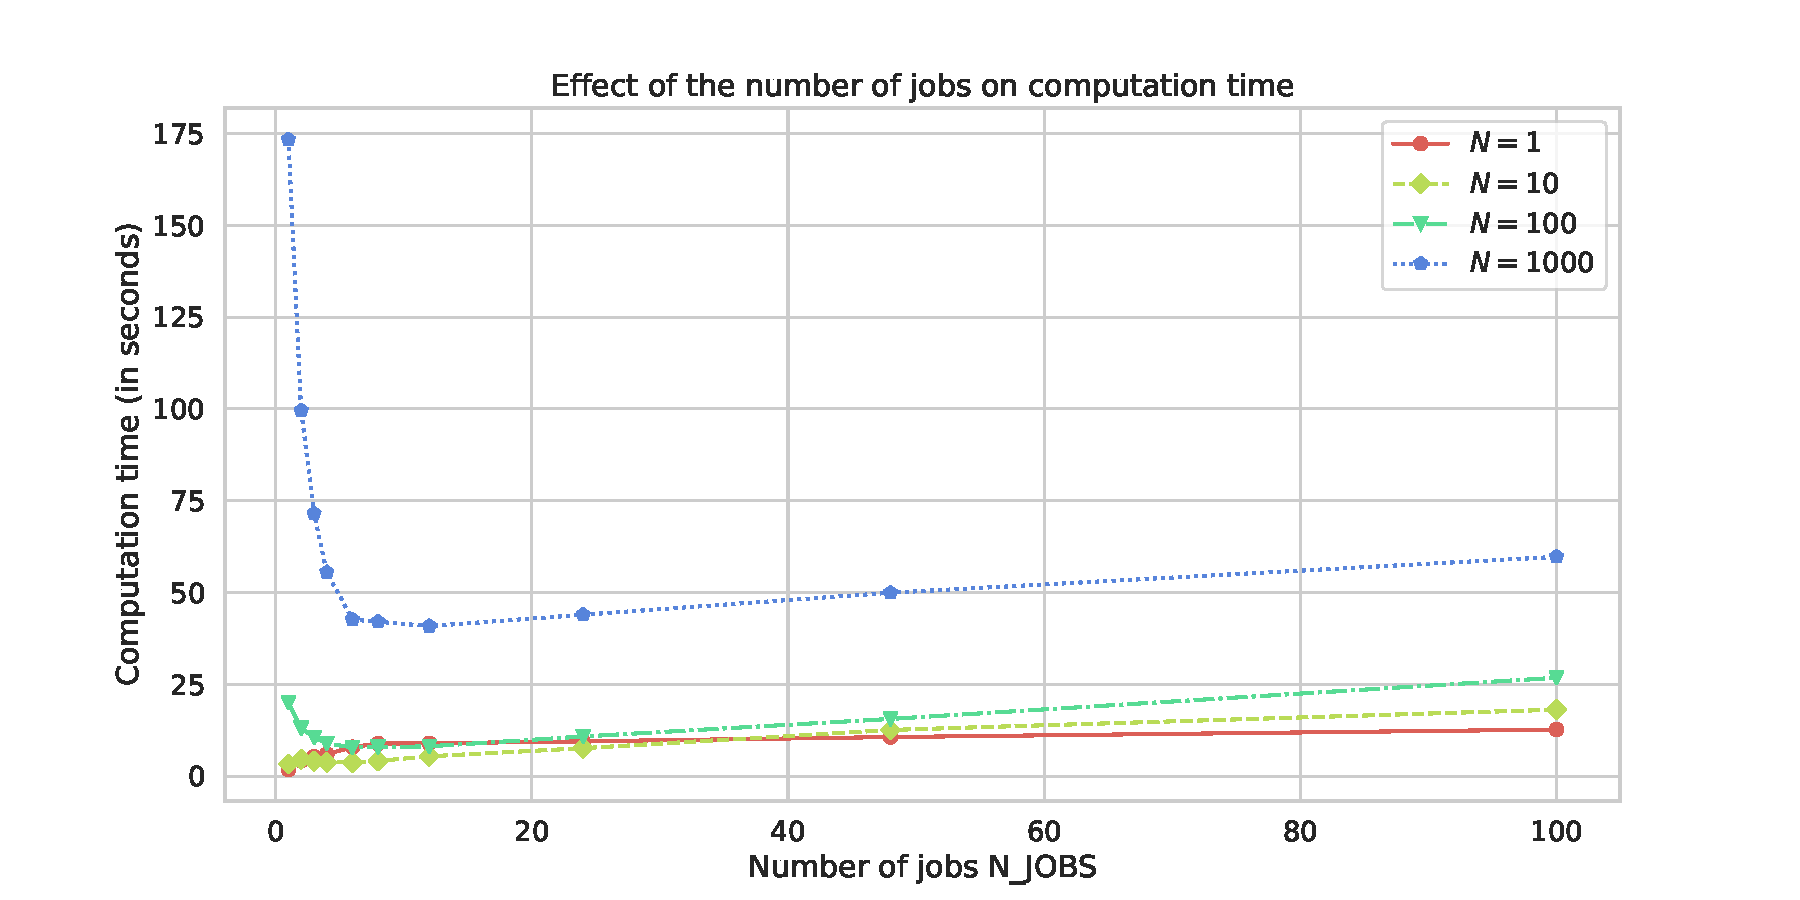
\includegraphics[width=0.85\linewidth]{analyze_speedup_as_nb_of_jobs.pdf}
% 	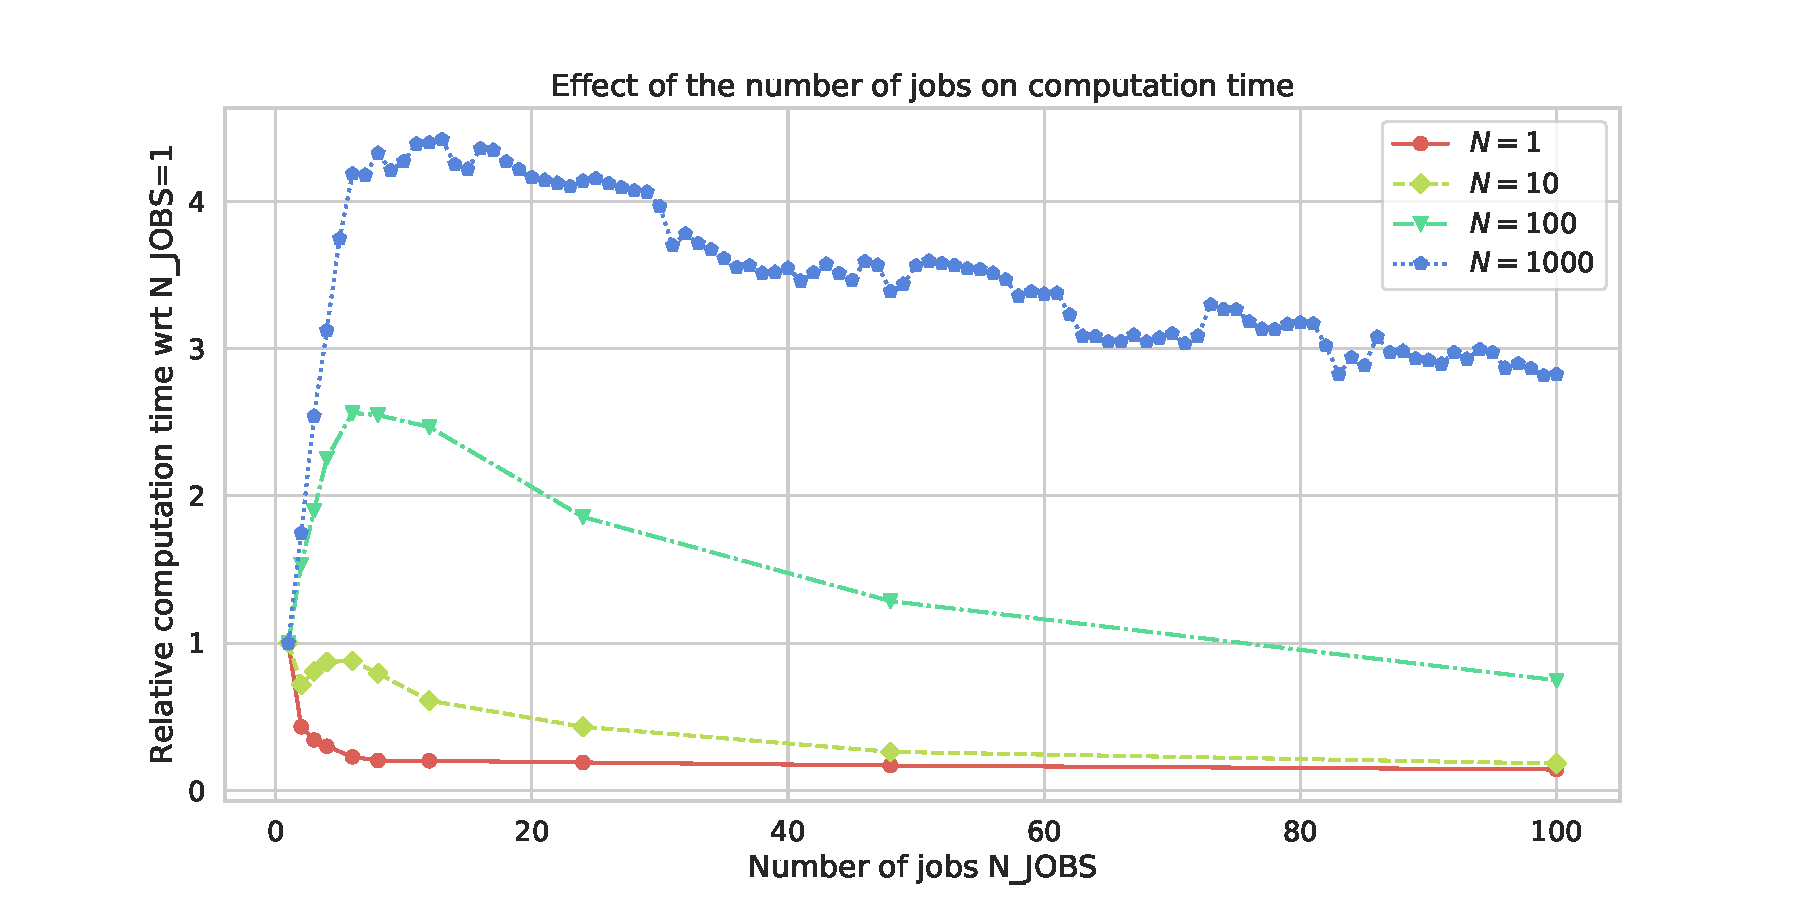
\includegraphics[width=1.10\linewidth]{analyze_speedup_as_nb_of_jobs_normalize.pdf}
% 	\caption{Relative gain on the running time in comparison to using one job, as a function of the number of jobs \texttt{N\_JOBS}, for a $n_{\text{cores}}=12$-core machine running the simulation of Code Example~\ref{lst:3:runOneCoreOrMore}.}
% 	\label{fig:3:analyze_speedup_as_nb_of_jobs}
% \end{figure}

% % for N in 1 10 100 1000; do for NJ in 1 12 100; do echo "With N=$N repetitions and N_JOBS=$NJ jobs..."; time NOPLOTS=True SAVEALL=False BAYES=False ARM_TYPE=Bernoulli N=$N T=1000 K=9 N_JOBS=$NJ python3 main.py configuration.py 2>/dev/null | grep "real "; done; done && FreeSMS.py "DONE"

% % $N=1$ repetition    & \SI{15}{\second}
% % & \SI{26}{\second} ($0.57 \%$)  % 15/26
% % & \SI{43}{\second} ($0.34 \%$)  % 15/43
% % \\
% % $N=10$ repetitions  & \SI{87}{\second}
% % & \SI{51}{\second} ($1.70 \%$)  % 87/51
% % & \SI{76}{\second} ($1.14 \%$)  % 87/76
% % \\
% % $N=100$ repetitions & \SI{749}{\second}
% % & \SI{272}{\second} ($2.75 \%$)  % 749/272
% % & \SI{308}{\second} ($2.43 \%$)  % 749/308
% % \\
% % $N=500$ repetitions & \SI{2944}{\second}
% % & \SI{1530}{\second} ($1.92 \%$)  % 2944/1530
% % & \SI{1846}{\second} ($1.59 \%$)  % 2944/1846



% % \TODOL{Pas sûr que ça vaille la peine d'inclure ce passage, c'est vraiment optionnel !}

% % % Explain why I didn't try more on parallelisation (eg on Grid5000 or other large scale computer).
% % \paragraph{Approaches we did not try.}
% % %
% % The two other approaches we could have consider is parallel computations running on not multiple cores but multiple machines, in a computer cluster, or parallel computations running in a Graphical Processing Unit (GPU).

% % $(i)$ I did not try to add in SMPyBandits the possibility to run simulations using a GPU, or any general purpose computation libraries offering a GPU-backend.
% % Initially designed for graphical simulations and mainly for video-games applications, the use of GPU for scientific computations have been gaining attention for numerical simulation in the research world since the last $15$ years, and NVidia CUDA for GPGPU (General Purpose GPU) started to become popular in $2011$.
% % Since $2016$, we saw a large press coverage as well as an extensive use in research of deep learning libraries that make general-purpose machine learning algorithms train on the GPU of a user's laptop or a cluster of GPU.
% % This success is mainly possible because of the heavy parallelism of such training algorithms, and the parallel nature of GPU.
% % To the best of the author knowledge, nobody has tried to implement high performance MAB simulations by using the ``parallelism power'' of a GPU (at least, no code for such experiments were made public in $2019$).
% % I worked on a GPU, implementing fluid dynamic simulations in an internship in $2012$, and I have since then kept a curiosity on how to use GPU-powered libraries and code.
% % I have contributed to and used famous deep-learning libraries, like Theano (\href{http://deeplearning.net/software/theano/}{\texttt{DeepLearning.net/software/theano}}) or Keras (\href{https://keras.io/}{\texttt{keras.io}}), and my limited knowledge on such libraries made me believe that it was not easy to use a GPU for bandit simulations, and most surely it would not have been worth the time.
% % I would be very curious to understand how a GPU could be used to implement highly efficient simulations for sequential learning problems, because it seemed hard whenever I thought about it.

% % $(ii)$ I also did not try to use any large scale computer cluster, even if I was aware of the possibility offered by the Grid 5000 project, for instance.
% % It is partly due to time constraint, as I would have been curious to try, but mainly because we found that it would not have helped us much to use a large scale cluster.
% % The main reason is that in the multi-armed bandit and sequential learning literature, most research papers do not even include an experimental section, and for the papers who did take the time to implement and test their proposed algorithms, it is almost done on just a few problems and for short- or medium- duration experiments.
% % For instance, the papers we consider to be the best ones regarding their empirical sections are \cite{LiuLeeShroff17,CaoZhenKvetonXie18}, for piece-wise stationary bandits, and they mainly consider reasonable problems of horizon $T=10000$ and no more than $1000$ independent repetitions. Each paper considers one harder problem, of horizon $T=1000000$ and less repetitions.
% % %
% % In each article written during my thesis, we included extensive numerical simulations, and even the longest ones (for \cite{Besson2019GLRT}) were short enough to run in less than $12$ hours on a $12$-core workstation, so we could run a few large-scale simulations over night.
% % For such reasons, we prefer to not try to run simulations on a cluster.
